\documentclass{report}
\usepackage{graphicx}
\usepackage{cite}
\usepackage{amsmath,amssymb,amsfonts}
\usepackage{algorithmic}
\usepackage{xcolor}
\usepackage[margin=1in]{geometry}
\usepackage{booktabs}
\usepackage{array}
\usepackage{float}
\usepackage{parskip}
\usepackage{url}
\usepackage[hidelinks]{hyperref}
\usepackage{changepage}
\usepackage{enumitem}
\usepackage{listings}
\usepackage{minted}
\usepackage{caption}
\usepackage{catchfile}
\usepackage{xfp}
\usepackage{arydshln}
\usepackage[toc,page]{appendix}

% \usemintedstyle{borland}
\renewcommand\listingscaption{Code}
\newcommand\indentWidthTwenty{20pt}
\newcommand\indentWidthForty{40pt}
\setcounter{secnumdepth}{3}
 

% Character and normal page count commands
\newcommand{\CharCountValue}{0}
\newcommand{\setcharcount}[1]{%
	\immediate\write18{texcount -1 -sum -merge -char -nobib #1.tex > #1-charcount.sum}%
	\CatchFileDef{\CharCountValue}{#1-charcount.sum}{}%
}
\newcommand{\pageestimate}{\fpeval{round(\CharCountValue/2400,2)}}


\begin{document}

\setcharcount{main}

\begin{titlepage}

    \begin{figure}
        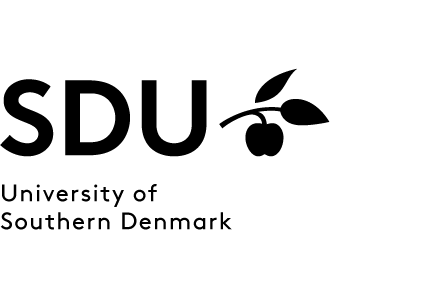
\includegraphics[width=8cm]{media/SDU_UK_1.png}
    \end{figure}

    % \vspace{0.5 cm}

    % {\scshape\LARGE University of Southern Denmark \par}

    % \vspace{0.5 cm}

    {\scshape\large Faculty of Engineering\par}
    {\scshape\large Mærsk Mc-Kinney Møller Institute\par}
    {\scshape\large Software Engineering\par}

    \vspace{1.5 cm}

    {\huge\bfseries Foundation Models for Reprogrammable \\Robotics through Knowledge Reuse\par}
    % {\large Master's Thesis\par}

    \vspace{2 cm}

    {\scshape\large Author:}\par
    {\large \textbf{Jacob Bregndahl Larsen}\\}
    {\large \texttt{jacla20@student.sdu.dk}\\}
    % {\large Exam nr.: 4138098\\}

    \vspace{0.5 cm}

    {\scshape\large Supervisor:}\par
    {\large \textbf{Mina Alipour}\\}
    {\large \texttt{mial@mmmi.sdu.dk}\\}

    \vfill

    {\large \CharCountValue characters}\\
    {\large \pageestimate\ pages (of 2400 characters)}\\


    {\large \today}

\end{titlepage}

\begin{abstract}
    Robotic programming remains a specialized and time-consuming activity, which limits reuse and rapid adaptation of existing robot solutions. This thesis investigates how large language models (LLMs) can support natural language-based comprehension and reprogrammability of robotic programs.

    The thesis contributes an architectural design exploration, and an implemented prototype that combines an agentic retrieval-augmented generation workflow with indexed robot-program and documentation corpora. The system includes an offline data pipeline for transformation, chunking, embedding, and ingestion; a FastAPI backend with retrieval tools and orchestration; and a frontend for program search and assistant-supported editing.

    The approach was evaluated through a controlled within-subject user study comparing a baseline workflow (UR Studio) with the proposed system. Results show that comprehension correctness remained near-perfect in both conditions, indicating that retrieval-supported assistant interaction can effectively support program understanding. However, the proposed system increased task completion time and reduced user confidence for comprehension tasks, with much of the time penalty linked to assistant latency and interaction overhead. For modification and reuse tasks, the proposed system underperformed the baseline in both correctness and completion time, particularly for structurally complex modifications.

    The findings indicate that LLM-based assistance is already promising for robotic program comprehension, but robust support for reprogrammability requires stronger grounding, improved retrieval quality and domain coverage, and a better-aligned editing abstraction than direct low-level program editing.
\end{abstract}
\newpage

%TC:ignore
\tableofcontents
%TC:endignore
\newpage

\chapter{Introduction} \label{chapter:introduction}
Industrial robotics has become a central component of modern automation systems, enabling high levels of precision and efficiency across domains such as assembly, packaging, logistics, and material handling. Advances in robotics and automation have contributed to a rapid global adoption of industrial robots, with more than 4.6 million robots operating in factories worldwide as of 2024 and annual installations exceeding 500,000 units for several consecutive years (2021-2024). \cite{IFR2025} This development reflects a broader industrial transition toward increasingly automated manufacturing.

Despite these advances, the development of robotic applications remain challenging. Robot programming is often a time-consuming and specialized process that requires expertise in proprietary programming languages and vendor-specific systems. As a result, adapting or reprogramming robotic systems for new tasks can involve significant engineering effort and cost. These challenges limit the scalability and flexibility of industrial automation and have motivated growing interest in approaches that simplify and accelerate robot programming. \cite{FERA2024}

One such initiative is the Fast and Efficient Robotic Automation via Reuse of Data (FERA) project, which investigates how existing robotic knowledge and program data can be reused to support the development of new automation solutions. \cite{FERA2024} Led by the University of Southern Denmark (SDU) in collaboration with industrial partners, including Universal Robots, the project aims to reduce programming effort, shorten development cycles, and lower implementation costs. Part of this effort is the development of a software platform that provides access to repositories of robotic programs and aims to enable improved reprogrammability and reuse across robotic applications.

At the same time, recent advances in large language models (LLMs) have transformed the field of software engineering. LLMs have demonstrated strong capabilities in natural language understanding and code-related tasks. \cite{chen2021evaluating, austin2021program} These capabilities have changed how developers interact with software systems by enabling natural language interfaces for generating, understanding, and modifying code.

The success of LLMs in software engineering suggests promising opportunities within robotic programming. By bridging human language and machine-executable instructions, LLMs may enable more intuitive interaction with robotic systems and reduce the technical barriers associated with robot programming. In this context, LLMs can support both comprehension and reprogrammability of robotic applications. They may assist users in understanding existing robot programs and documentation through summarization and explanation, while also enabling the generation or modification of robot code from high-level natural language instructions. Such capabilities align closely with the objectives of the FERA project, where effective reuse of robotic knowledge depends on making existing solutions accessible, understandable, and adaptable.

However, applying LLMs within robotics also introduces significant challenges. Industrial robotic systems operate in constrained and safety-critical environments where reliability, correctness, and predictability are essential. Consequently, the integration of LLMs into robotic programming workflows requires careful consideration.


\section{Problem Statement} \label{sec:introduction:problem-statement}
This thesis investigates how large language models can be utilized to support natural language-based comprehension and reprogrammability of robotic programs, with a focus on leveraging existing data and documentation. By exploring methods for integrating LLMs with repositories of robotic knowledge, this thesis contributes (1) an architectural design exploration, that includes agentic retrieval augmented generation (RAG), in a constrained robotics domain, (2) an implemented prototype, and (3) an empirical user study that reveals specific limitations and design pitfalls of this approach.

This thesis is guided by the following research question (RQ):
\begin{adjustwidth}{\indentWidthTwenty}{\indentWidthTwenty}
    \textit{\textbf{RQ:} How can LLMs be used to support natural language-based comprehension and reprogrammability of robotic programs?}
\end{adjustwidth}

As well as the following sub research questions:
\begin{adjustwidth}{\indentWidthTwenty}{\indentWidthTwenty}
    \textit{\textbf{RQ1:} How does the proposed system influence the correctness of comprehension of robotic programs?}
\end{adjustwidth}
\begin{adjustwidth}{\indentWidthTwenty}{\indentWidthTwenty}
    \textit{\textbf{RQ2:} How does the proposed system influence the time required for comprehension of robotic programs?}
\end{adjustwidth}
\begin{adjustwidth}{\indentWidthTwenty}{\indentWidthTwenty}
    \textit{\textbf{RQ3:} How does the proposed system influence the correctness of modification and reuse of robot programs?}
\end{adjustwidth}
\begin{adjustwidth}{\indentWidthTwenty}{\indentWidthTwenty}
    \textit{\textbf{RQ4:} How does the proposed system influence the time required in the modification and reuse of robot programs?}
\end{adjustwidth}

\section{Scope} \label{sec:introduction:scope}
The scope of this thesis is shaped by practical constraints related to data availability and computational resources, which define what can realistically be explored within the context of this work.

The project was expected to utilize the robotic program repository from the FERA project mentioned above. However, at the time of development, the repository was not yet available for use. Thus, this thesis is developed using a limited dataset of robotics programs that does not fully represent the diversity of robotic solutions. This severely limits the design approaches that can be explored and the evaluation of the developed system. In addition, computational constraints further bound the design space. Approaches that require significant resource demands are not aligned with the practical limits of this master's thesis project. As a result, the project aims to explore solutions that can operate within these constraints while still effectively leveraging the available data.

The scope is further constrained to a specific robotics domain. The project focuses exclusively on robotic data originating from Universal Robots systems, as this is the data available within the project context. Consequently, the system is not intended to provide a general solution applicable to all robot brands, programming environments, or hardware configurations. Instead, it aims to investigate how the proposed concepts can be applied within a well-defined and consistent domain where data characteristics are known.
\chapter{Background} \label{sec:background}
This chapter introduces the background information needed to understand the robot programming concepts mentioned in this thesis.

% \section{Terminology}
% \subsection{Large Language Models}
% Large Language Models (LLMs) are a class of machine learning models designed to process, generate, and reason over natural language. They are typically based on deep neural network architectures, most commonly the transformer architecture, and are trained on large-scale text corpora using self-supervised learning objectives. By learning statistical patterns in language, LLMs can perform a wide range of tasks, including text generation, summarization, translation, question answering, and code synthesis.

% At a high level, LLMs operate by modeling the probability distribution of sequences of tokens. Given a sequence of input tokens, the model predicts the probability of the next token in the sequence. During training, the model is optimized to maximize the likelihood of correct next-token predictions across large datasets. This objective enables the model to capture syntactic structure, semantic relationships, and contextual dependencies within language.

% The core architectural component enabling this behavior is the transformer, which relies on mechanisms such as self-attention to weigh the relevance of different tokens in a sequence. Self-attention allows the model to dynamically focus on different parts of the input when generating each token, enabling it to capture long-range dependencies more effectively than earlier sequence models.

% Content generation in LLMs is performed in an autoregressive manner. Starting from an initial input (prompt), the model repeatedly predicts the next token based on the previously generated tokens and the input context. At each step, the model produces a probability distribution over its vocabulary, and a token is selected according to a decoding strategy. This iterative process continues until a stopping condition is met, such as reaching a maximum length or generating a special end-of-sequence token.

% Because LLMs are statistical models, their outputs are inherently non-deterministic under most decoding strategies. When sampling-based methods are used, the same prompt can produce different outputs across multiple runs, as token selection is influenced by probabilistic choices. Even when deterministic decoding strategies are applied, minor changes in input or configuration can lead to different outputs due to the sensitivity of the underlying probability distributions.

% LLMs are categorized based on their functionality or optimization objective:
% \begin{itemize}
%     \item \textbf{Text Models:} These models are optimized for natural language understanding and generation tasks. They are commonly used for conversation, summarization, and content generation.
%     \item \textbf{Embedding Models:} These models map text into high-dimensional vector representations. The resulting embeddings capture semantic similarity and are used in tasks such as information retrieval, clustering, and recommendation systems.
%     \item \textbf{Code Models:} These models are trained on source code and natural language descriptions to support tasks such as code generation, completion, refactoring, and documentation.
% \end{itemize}

% Despite differences in specialization, these models share common underlying mechanisms and concepts, which are described in the following subsections.

% \paragraph{Tokens}~\\
% Tokens are the fundamental units of text processed by language models. Instead of operating directly on raw characters or words, LLMs segment input text into tokens, which may correspond to words, subwords, or individual characters depending on the tokenization scheme. For example, a word may be split into multiple subword tokens to efficiently represent rare or complex vocabulary.

% Tokenization enables models to operate over a fixed vocabulary while maintaining flexibility in representing diverse linguistic inputs. The number of tokens in an input directly affects computational cost and model constraints, as most models impose limits on how many tokens can be processed simultaneously.

% \paragraph{Context Window}~\\
% The context window refers to the maximum number of tokens a model can consider in a single input sequence. This includes both the prompt (input) and the generated output. The size of the context window is a critical factor in determining how much information the model can use when generating responses.

% A larger context window allows the model to incorporate more prior information, enabling better handling of long documents, multi-turn conversations, and complex reasoning tasks. However, increasing the context window also raises computational and memory requirements. Consequently, practical systems must balance context length with efficiency.

% \paragraph{Prompts}~\\
% Prompts are structured inputs provided to a language model to guide its behavior and outputs. A prompt may consist of instructions, examples, or contextual information that influence how the model interprets and responds to a task.

% Prompt design, often referred to as prompt engineering, plays a significant role in eliciting desired behavior from LLMs. Techniques such as zero-shot prompting (no examples), few-shot prompting (providing examples), and instruction-based prompting are commonly used to improve performance on specific tasks without retraining the model.

% Prompts can also define system-level constraints, such as tone, format, or domain-specific requirements, making them a flexible interface for controlling model outputs.

% \paragraph{Fine-tuning}~\\
% Fine-tuning is the process of adapting a pre-trained language model to a specific task or domain by continuing training on a smaller, task-specific dataset. While base models learn general language patterns from large corpora, fine-tuning refines their behavior using examples that reflect the desired input-output relationship.

% This is typically done by optimizing the same next-token prediction objective, but on more narrowly defined data. Fine-tuning can involve updating all model parameters (full fine-tuning) or only a subset (parameter-efficient methods), depending on computational constraints. Variants such as instruction tuning and reinforcement learning from human feedback further improve a model's ability to follow instructions and align with human preferences.

% Although fine-tuning can significantly improve task performance, it introduces challenges such as overfitting and potential loss of general capabilities.



\section{Programming of Universal Robots Manipulators}
Universal Robots (UR) manipulators support both graphical and textual approaches to robot programming. In practice, these approaches are closely integrated: robot applications are commonly developed through the graphical teach pendant environment, while execution on the robot controller is ultimately represented internally as URScript instructions. \cite{MartinRytterFiveWaysToProgramACobot}

The primary development interface for UR systems is the teach pendant, which provides a graphical, node-based programming environment for constructing robot behavior. Programs are created by composing and configuring nodes representing actions such as robot motion, waiting conditions, control flow, and tool operations. This interface is designed to be user-friendly and accessible, allowing users to define waypoints directly on the robot and configure motion parameters through graphical forms.

Programs created through the teach pendant are stored as project artifacts, represented as \texttt{.urpx} files. A \texttt{.urpx} file captures the complete program definition produced within the graphical environment, including the hierarchy of program nodes, configured parameters, waypoint references, and metadata required by the controller. Structurally, a UR program can be viewed as a hierarchical tree rooted in a main program node, where child nodes define execution order, control flow, and robot actions. Motion-related nodes typically reference named waypoints together with parameters such as speed, acceleration, blending radius, and movement type, while additional nodes may define loops, conditional logic, wait conditions, and I/O operations.

The functionality of the programming environment can further be extended through URCaps, which are software extensions installed directly on the robot controller. URCaps enable developers and hardware vendors to integrate custom functionality into the teach pendant environment by introducing new program nodes and configuration interfaces beyond the standard functionality provided by the controller. In industrial applications, URCaps are commonly used to integrate peripherals and process-specific operations, including grippers, vision systems and sensors. Since URCaps integrate directly into the graphical workflow, their functionality also becomes embedded within the resulting program structure and execution model.

Although the graphical programming interface simplifies robot development, more advanced robotic applications often require functionality and flexibility beyond what is practical to express through graphical nodes alone. For such applications, developers frequently rely on URScript, the domain-specific scripting language used internally by UR controllers. URScript resembles Python syntactically. Compared to graphical programming, URScript provides finer-grained control and greater expressiveness for implementing reusable logic, dynamic execution behavior, and integration with external systems. URScript programs may be written manually or generated automatically from higher-level representations, including teach pendant programs and URCaps.

In addition to teach pendant programming and URScript, UR manipulators also support external control through network-based communication interfaces. External applications can exchange data with the controller and issue commands programmatically from separate computing systems. This capability is particularly valuable in research and experimental environments, where robotic systems are frequently integrated with external software. One example of this is the \texttt{ur\_rtde} library, which provides Python and C++ interfaces for communication with UR controllers through the Real-Time Data Exchange (RTDE) protocol \cite{lindvig2025ur_rtde}.
\chapter{Related Work} \label{chapter:related-work}
This chapter provides an overview of the related research within the field of AI-assisted software development and robotic application development.

\section{Methodology}
This section describes the methodology used to identify and analyze the presented literature below. A systematic search was conducted across the SDU Library database, which include numerous scientific databases. \cite{SDU-Library} However, the search produced few directly relevant studies on the use of LLMs for development of robotic programs. Thus, the search was split into two focused systematic searches, one on AI-assisted software development and one on robotic solution development and reuse of data within robotics. The search was conducted using SDU Library and Google Scholar with keywords such as "AI assisted development" and "robotic data reuse". \cite{google-scholar} The search was supplemented with reverse snowballing. Only English language papers were included, and newer studies with more citations was prioritized. Studies were screened based on title, abstract, and full-text assessment for relevance.


\section{AI-Assisted Software Development}
Large language models have changed software development by making code generation and reasoning accessible through natural language interaction. AI-powered code assistants such as GitHub Copilot embed these capabilities directly in development environments, where they assist with development from local context. \cite{GitHubCopilot2026} Empirical studies report measurable productivity gains for routine and well-specified tasks, while benchmark evaluations show that code models can solve a meaningful subset of programming problems, although performance still depends strongly on task complexity and specification quality. \cite{bird2022taking, chen2021evaluating, austin2021program}

Their use extends beyond code synthesis. AI assistants are used for testing, debugging, maintenance, documentation, and explanation of unfamiliar code or technologies, which positions them as interactive knowledge aids as well as automation tools. \cite{barke2023grounded, vaithilingam2022expectation} Studies show they can support novice programmers with examples and feedback for comprehension, but they also risk encouraging shallow understanding and overreliance when generated code is accepted without reflection. \cite{kazemitabaar2023studying}

These benefits are accompanied by concerns about reliability and governance. AI-generated code may contain subtle bugs, inefficiencies, or security vulnerabilities without explicit warning, which means human review and validation remain necessary. \cite{pearce2025asleep}

\newpage
\subsection{Assistants and Agents}
Artificial intelligence systems based on large language models are commonly described in terms of two roles: AI assistants and AI agents. \cite{IBM2026AIAgentsVsAIAssistants} Although this distinction is useful for conceptual clarity, in practice the boundary between them is increasingly fluid. \cite{yao2022react} Both categories rely on similar underlying technologies, yet they differ in how these capabilities are organized, how control is distributed, and how tasks are executed within the system.

AI assistants are interactive systems that respond to user input in a direct and context-aware manner. Their primary role is to support users by generating relevant outputs, such as text or code, based on prompts. The interaction model is fundamentally reactive: each response is triggered by explicit user input, and the system does not independently pursue goals beyond the current exchange. While assistants may retain short-term conversational context, their behavior is largely constrained to a prompt-response cycle. As a result, they are well suited for tasks that require human oversight, iterative refinement, and clear user control, such as programming support, writing assistance, or question answering.

AI agents, in contrast, represent a shift toward more autonomous and goal-oriented systems. In this approach, a language model is embedded within a broader architecture that enables planning, state management, and interaction with external tools. Agents can decompose complex objectives into smaller steps, execute these steps sequentially, and adapt their behavior based on intermediate results. This is achieved through the integration of additional components, such as memory mechanisms for maintaining context across interactions, tool interfaces for accessing external functionality, and control loops that govern decision-making. Consequently, agents are capable of handling multistep workflows and operating with a degree of independence from direct user input.

Despite these conceptual differences, the line between assistants and agents is increasingly blurred. Modern systems often combine characteristics of both, resulting in hybrid architectures. An assistant may incorporate agent-like features, such as maintaining longer-term context, suggesting proactive actions, or coordinating subtasks behind the scenes. Conversely, agents may expose assistant-like interfaces when interacting with users, relying on dialogue to clarify goals or refine outputs. This convergence reflects a broader trend in AI system design, where interaction and autonomy are not treated as mutually exclusive, but rather as complementary capabilities.

\subsection{Specialized Models}
At the core of AI assistants lie foundation models based on the transformer architecture introduced by Attention Is All You Need. \cite{vaswani2017attention} Building upon these are an evolution of the general-purpose language models, often referred to as code models. These models are specialized models tailored for software engineering tasks. While they are built upon the same underlying architectures as general large language models, they are trained on large corpora of code and natural language, allowing them to learn statistical patterns that generalize across coding tasks. \cite{chen2021evaluating}

The primary benefit of this specialization is the acquisition of domain-specific knowledge. Code models are better equipped than general LLMs to understand programming constructs, adhere to syntax and semantic constraints, and generate outputs that reflect software engineering practices. This results in improved performance across a wide range of development tasks and enables their integration into tools that support developer productivity, such as intelligent code completion and automated documentation generation. \cite{chen2021evaluating ,li2022competition} However, coding models suffer from the same challenges as other LLMs, including hallucinations, outdated knowledge, and difficulties handling project-specific or proprietary contexts. \cite{ji2023survey, gao2023retrieval} These challenges have motivated the integration of external knowledge sources.

\newpage
\subsection{Retrieval-Augmented Generation} \label{sec:related-work:RAG}
Retrieval-Augmented Generation (RAG) is a technique for enhancing LLMs by enabling them to access and incorporate external knowledge at inference time. \cite{lewis2020retrieval} Rather than relying solely on the information encoded in model parameters during training, RAG systems retrieve relevant documents from a knowledge source, such as a database, document collection, or code repository, and use this information to inform the generated response. At a high level, RAG operates in two stages: a retrieval step, where a user query is used to identify relevant pieces of information, and a generation step, where the retrieved content is incorporated into the model's input context to produce a response. This combination allows RAG systems to improve factual accuracy, remain up-to-date without retraining, and ground their outputs in verifiable sources. Over time, this basic retrieve-then-generate paradigm has evolved into a range of increasingly sophisticated architectures that extend how retrieval is performed, integrated, and controlled. Recent surveys categorize this evolution into distinct categories, naive RAG, advanced RAG, modular RAG, and agentic RAG, each addressing specific limitations of earlier designs. \cite{gao2023retrieval, singh2025agentic} Naive RAG treats retrieval as a single, static preprocessing step; advanced RAG refines it through multi-stage pipelines and iterative reasoning; modular RAG generalizes the architecture into flexible components; and agentic RAG elevates retrieval to a dynamic, decision-driven process embedded within autonomous agents.

\subsection{Agentic Capabilities for AI Assistants}
As mentioned above, the line between AI assistants and AI agents are increasingly blurred. The emergence of agentic capabilities marks a significant shift in the design and functionality of AI assistants within software engineering. While early generations of assistants were predominantly reactive, limited to single-turn interactions and narrow task execution, recent advances in LLMs have enabled systems that exhibit goal-directed, iterative, and context-aware behavior. These agentic systems extend beyond prompt-response paradigms by incorporating mechanisms for planning, tool use, and self-reflection, thereby aligning more closely with traditional notions of autonomous agents in artificial intelligence. This evolution reflects a convergence between interactive assistants and autonomous software agents, where the distinction increasingly depends on the degree of autonomy and environmental interaction.

A central characteristic of agentic AI assistants is their ability to decompose complex tasks into sequences of intermediate steps and to dynamically adapt these plans based on feedback from the environment. Approaches such as ReAct integrate reasoning and acting by interleaving natural language "thoughts" with concrete actions, enabling models to query external systems, retrieve information, or execute code as part of their problem-solving process. \cite{yao2022react} This paradigm has proven particularly effective in software engineering contexts, where tasks such as debugging, test generation, and refactoring require iterative exploration and validation.

Tool augmentation is a foundational enabler of these capabilities. By granting AI assistants access to external tools, such as compilers, interpreters, static analysis frameworks, and documentation retrieval systems, researchers have significantly expanded the operational scope of LLM-based systems. In this setting, tool invocation becomes an integral part of the reasoning process, requiring the model to select appropriate tools, construct valid inputs, and interpret outputs correctly. Frameworks for tool-augmented reasoning formalize this interaction, often treating tool selection as a decision-making problem guided by the model's internal representations. \cite{schick2023toolformer} While this integration enhances practical utility, it also introduces new challenges related to robustness and security. Incorrect tool usage can lead to failures, and unrestricted access to external systems raises concerns about data leakage, privilege escalation, and unintended side effects.

Another important dimension of agentic systems is their capacity for self-reflection and iterative improvement. Techniques such as Reflexion and self-consistency prompting enable models to evaluate their own outputs and revise them in subsequent iterations, effectively implementing a form of meta-reasoning. \cite{shinn2023reflexion} In software engineering applications, this capability is particularly valuable for tasks that benefit from trial-and-error, such as synthesizing correct programs or generating test cases that satisfy specific coverage criteria. By maintaining internal feedback loops, agentic assistants can progressively refine their outputs, thereby improving reliability without requiring external supervision at every step.

The concept of multi-agent collaboration further extends the agentic paradigm by distributing responsibilities across multiple specialized agents. In such systems, distinct agents may be responsible for planning, implementation, testing, and verification, communicating through structured protocols or shared memory representations. \cite{hong2023metagpt} This modularization can improve scalability and allow for more interpretable workflows, as each agent operates within a well-defined role. However, coordination among agents introduces additional complexity, including synchronization overhead, communication bottlenecks, and the risk of error propagation across agent boundaries.


\section{Robotic Application Development}
An automation solution for an industrial task consists of both hardware and software. The hardware may include the robot manipulator, grippers, peripheral devices, and safety components, while the software spans both system software and the user program that makes the specific application perform the intended task.

Several approaches have attempted to make the robot programming easier. User-interaction-based Programming by Demonstration \cite{ravichandar2020recent} and abstraction-based Programming by Skills \cite{saukkoriipi2020programming}, aim to raise the level of abstraction in robot programming and reduce the amount of low-level engineering work required from the user. However, these lines of work also illustrate a persistent limitation: it remains difficult to formalize and capture the broad practical knowledge needed to make such approaches work reliably at scale.

In robotics, software reuse has also been explored as a way to accelerate development and improve system reliability. Much of this effort has focused on ROS, the open-source Robot Operating System. \cite{quigley2009ros} Today, the ROS ecosystem allows roboticists to assemble complete robotic systems by integrating existing software modules instead of developing all functionality from the ground up. \cite{kolak2020takes} However, this approach to reuse is primarily aimed at expert roboticists and program reuse remains difficult in practice. Estefo et al. surveyed 119 ROS users and found that more than 70\% had experienced failing to successfully reuse existing packages and participants reporting the search process as time-consuming and often unproductive, often due to challenges such as abandoned packages. \cite{estefo2019robot}

In industrial applications, Universal Robots introduced "URCaps", software extensions that simplify the integration of peripherals into robot systems. While this reduces the complexity of building automation applications, it does not directly support the reuse of previously developed application code.

Recent advances in machine learning and large-scale foundation models have nevertheless renewed interest in automating parts of robotic application development. A prominent example is SayCan, which combines large language models with robot affordance functions to generate high-level action sequences grounded in the robot's actual capabilities. \cite{brohan2023can} In SayCan, the language model proposes candidate actions while learned value functions estimate whether these actions are feasible in the current environment. This enables the system to decompose abstract natural-language instructions into executable robot behaviors. The work demonstrates that large language models can contribute semantic and procedural knowledge to robotic planning, but it also highlights a limitation: the resulting solutions still depend on predefined low-level skills and carefully engineered grounding mechanisms. The generated behavior therefore remains constrained by the available skills, training data, and environment-specific affordance models.

Subsequent work has extended this direction toward increasingly general robot policies. RT-1 introduced a large-scale transformer-based robotic control architecture trained on 130,000 real-world demonstrations covering more than 700 tasks. \cite{brohan2022rt1} Rather than focusing only on symbolic task planning, RT-1 directly maps vision and language inputs to robot actions using a unified transformer architecture. The study demonstrated improved robustness and generalization across tasks, environments, and objects, suggesting that large and diverse datasets can support more reusable robot behaviors.

RT-2 further extends this approach by integrating vision-language models trained on Internet-scale data directly into robotic control. \cite{zitkovich2023rt2} The model represents robot actions as textual tokens, allowing robotic trajectories and web-scale vision-language data to be trained within a shared framework. This enables forms of semantic reasoning and generalization that were previously difficult to achieve in robotics, including reasoning about novel objects, symbols, and relationships between objects. RT-2 demonstrates that pretrained vision-language models can transfer broad semantic knowledge into robotic behavior generation.

Together, these approaches represent a significant shift in robotics research from manually engineered task logic toward data-driven policy generation and semantic reasoning. Such systems are particularly promising for robots operating in dynamic and unpredictable environments, where flexibility, natural-language interaction, and adaptation to novel situations are important capabilities. However, industrial automation environments often prioritize different requirements, including deterministic execution, repeatability, and compatibility with established safety and validation procedures. Consequently, despite major advances in embodied AI and robotic foundation models, the development of industrial robotic applications still relies heavily on explicit robot programs and engineering expertise. This suggests that there remains a need for approaches that support the creation, comprehension, and reuse of robot program code within existing industrial development practices.


% \section{Contribution}
% Consequently, this thesis aims to contribute to the existing body of knowledge by investigating how large language models and robotic data can support the development and understanding of robotic programs.
\chapter{Requirement Engineering}
This chapter describes the requirement engineering process, including requirements elicitation, analysis, and specification. The goal of this process was to identify and define the requirements that would guide the design of the system.


\section{Requirements Elicitation}
During the requirement elicitation phase, functional and non-functional requirements were identified through an initial brainstorming session, informed by the authors' domain knowledge in robotics. This was complemented by a review of relevant literature and existing work to extract common requirements and established best practices for comparable systems (see Chapter \ref{chapter:related-work}). The process was iterative, with requirements continuously refined as the understanding of the problem domain and potential solution space evolved. This resulted in an initial set of requirements that informed the subsequent requirement analysis.

It is acknowledged that the absence of direct input from end-users and stakeholders introduces limitations. In particular, misalignment between system functionality and user needs may lead to reduced usability and thus increased development effort due to rework of the system. Incorporating stakeholder feedback during the requirements phase, through methods such as interviews, surveys, or workshops, would help mitigate these risks and likely improve the overall quality of the system.


\section{Requirements Analysis}
\subsection{Use Cases}
To further refine and structure the system requirements, use cases were employed. Use cases provide a scenario-based perspective of system functionality by describing how actors interact with the system to achieve specific goals. This approach complements the previously identified requirements. The development of the use cases followed a systematic process described below.

First, the relevant actors were identified. Actors represent entities that interact with the system, either as users or as external systems. In this project, two primary actors were defined: the Developer, representing the end-user interacting directly with the system, and the LLM Provider, representing the external service supplying large language model capabilities. The FERA vector database was also considered as an actor, but it was ultimately not included as the database is not part of this project as described in the scope (see Section \ref{sec:introduction:scope}).

\begin{table}[H]
    \centering
    \begin{tabular}{p{2.5cm}p{11.5cm}}
        \toprule
        \textbf{Actor} & \textbf{Description}                                                                                       \\
        \midrule
        Developer      & A user who interacts with the system to search, understand, and edit robotic programs.                     \\
        LLM Provider   & An external service that provides large language model capabilities to support the system's functionality. \\
        \bottomrule
    \end{tabular}
    \caption{List of actors.}
    \label{tab:requirement-engineering:actors}
\end{table}

\vspace{-0.1cm}
Next, the use cases were identified. These correspond to the main functionalities the system must support. For the Developer, the primary use cases include searching, editing, uploading, and exporting robot programs. In addition, the system provides LLM-assisted functionality through the use case "Get LLM assisted support". This captures interactions where the system leverages the LLM to assist the user. This high-level LLM-assisted use case was further refined into more specific functionalities, namely: answering user questions, generating robot programs, modifying existing programs, and debugging robot programs. These represent distinct goals that can be achieved through the LLM integration. A validate/simulate robot program use case was also considered, but ultimately not included as it goes beyond the scope of this project.

\begin{table}[H]
    \centering
    \begin{tabular}{p{4cm}p{10cm}}
        \toprule
        \textbf{Use Case}        & \textbf{Description}                                                                                                                                     \\
        \midrule
        Search robot programs    & The Developer can search for relevant robotic programs based on natural language queries.                                                                \\
        Edit robot program       & The Developer can edit existing robotic programs to adapt them to new contexts.                                                                          \\
        Upload robot program     & The Developer can upload their own robotic programs to edit using the system and for inclusion in the repositories and identification in future queries. \\
        Export robot program     & The Developer can export robotic programs from the system.                                                                                               \\
        Get LLM assisted support & The Developer can receive assistance from the LLM to support various tasks related to robotic program development.                                       \\
        Answer user questions    & The system can answer user questions related to robotic programs and documentation using the LLM.                                                        \\
        Generate robot program   & The system can generate new robotic programs based on user input using the LLM.                                                                          \\
        Modify existing program  & The system can modify existing robotic programs based on user input using the LLM.                                                                       \\
        Debug robot program      & The system can assist in debugging robotic programs by identifying potential issues and suggesting fixes using the LLM.                                  \\
        \bottomrule
    \end{tabular}
    \caption{List of use cases.}
    \label{tab:requirement-engineering:use-cases}
\end{table}

\vspace{-0.1cm}
Following this, associations between actors and use cases were established. The Developer is connected to all primary use cases, reflecting direct interaction with the system's features. The LLM Provider is associated with the LLM-assisted support functionalities, indicating that these capabilities depend on an external service.

A system boundary was then defined to clearly distinguish between the internal system functionality and external actors. All use cases are contained within this boundary, while the actors remain outside, interacting with the system through defined interfaces.

Finally, relationships between use cases were modeled. The "Get LLM assisted support" use case is represented as an extension of the "Edit robot program" use case, indicating that assistance is an optional feature that can enhance the editing process. Additionally, the more specific LLM-related use cases can be seen as generalizations of the assistance functionality, providing more detailed descriptions of how the system supports the user.

\subsection{Use Case Diagram}
The resulting use case diagram is shown in Figure \ref{fig:requirement-engineering:use-case-diagram}. It provides an overview of the system's functionality, the involved actors, and the relationships between different interactions. This diagram contributes to refining the initial requirements by clarifying system functionality and interactions, and serves as a foundation for the subsequent system design.

\begin{figure}[H]
    \centering
    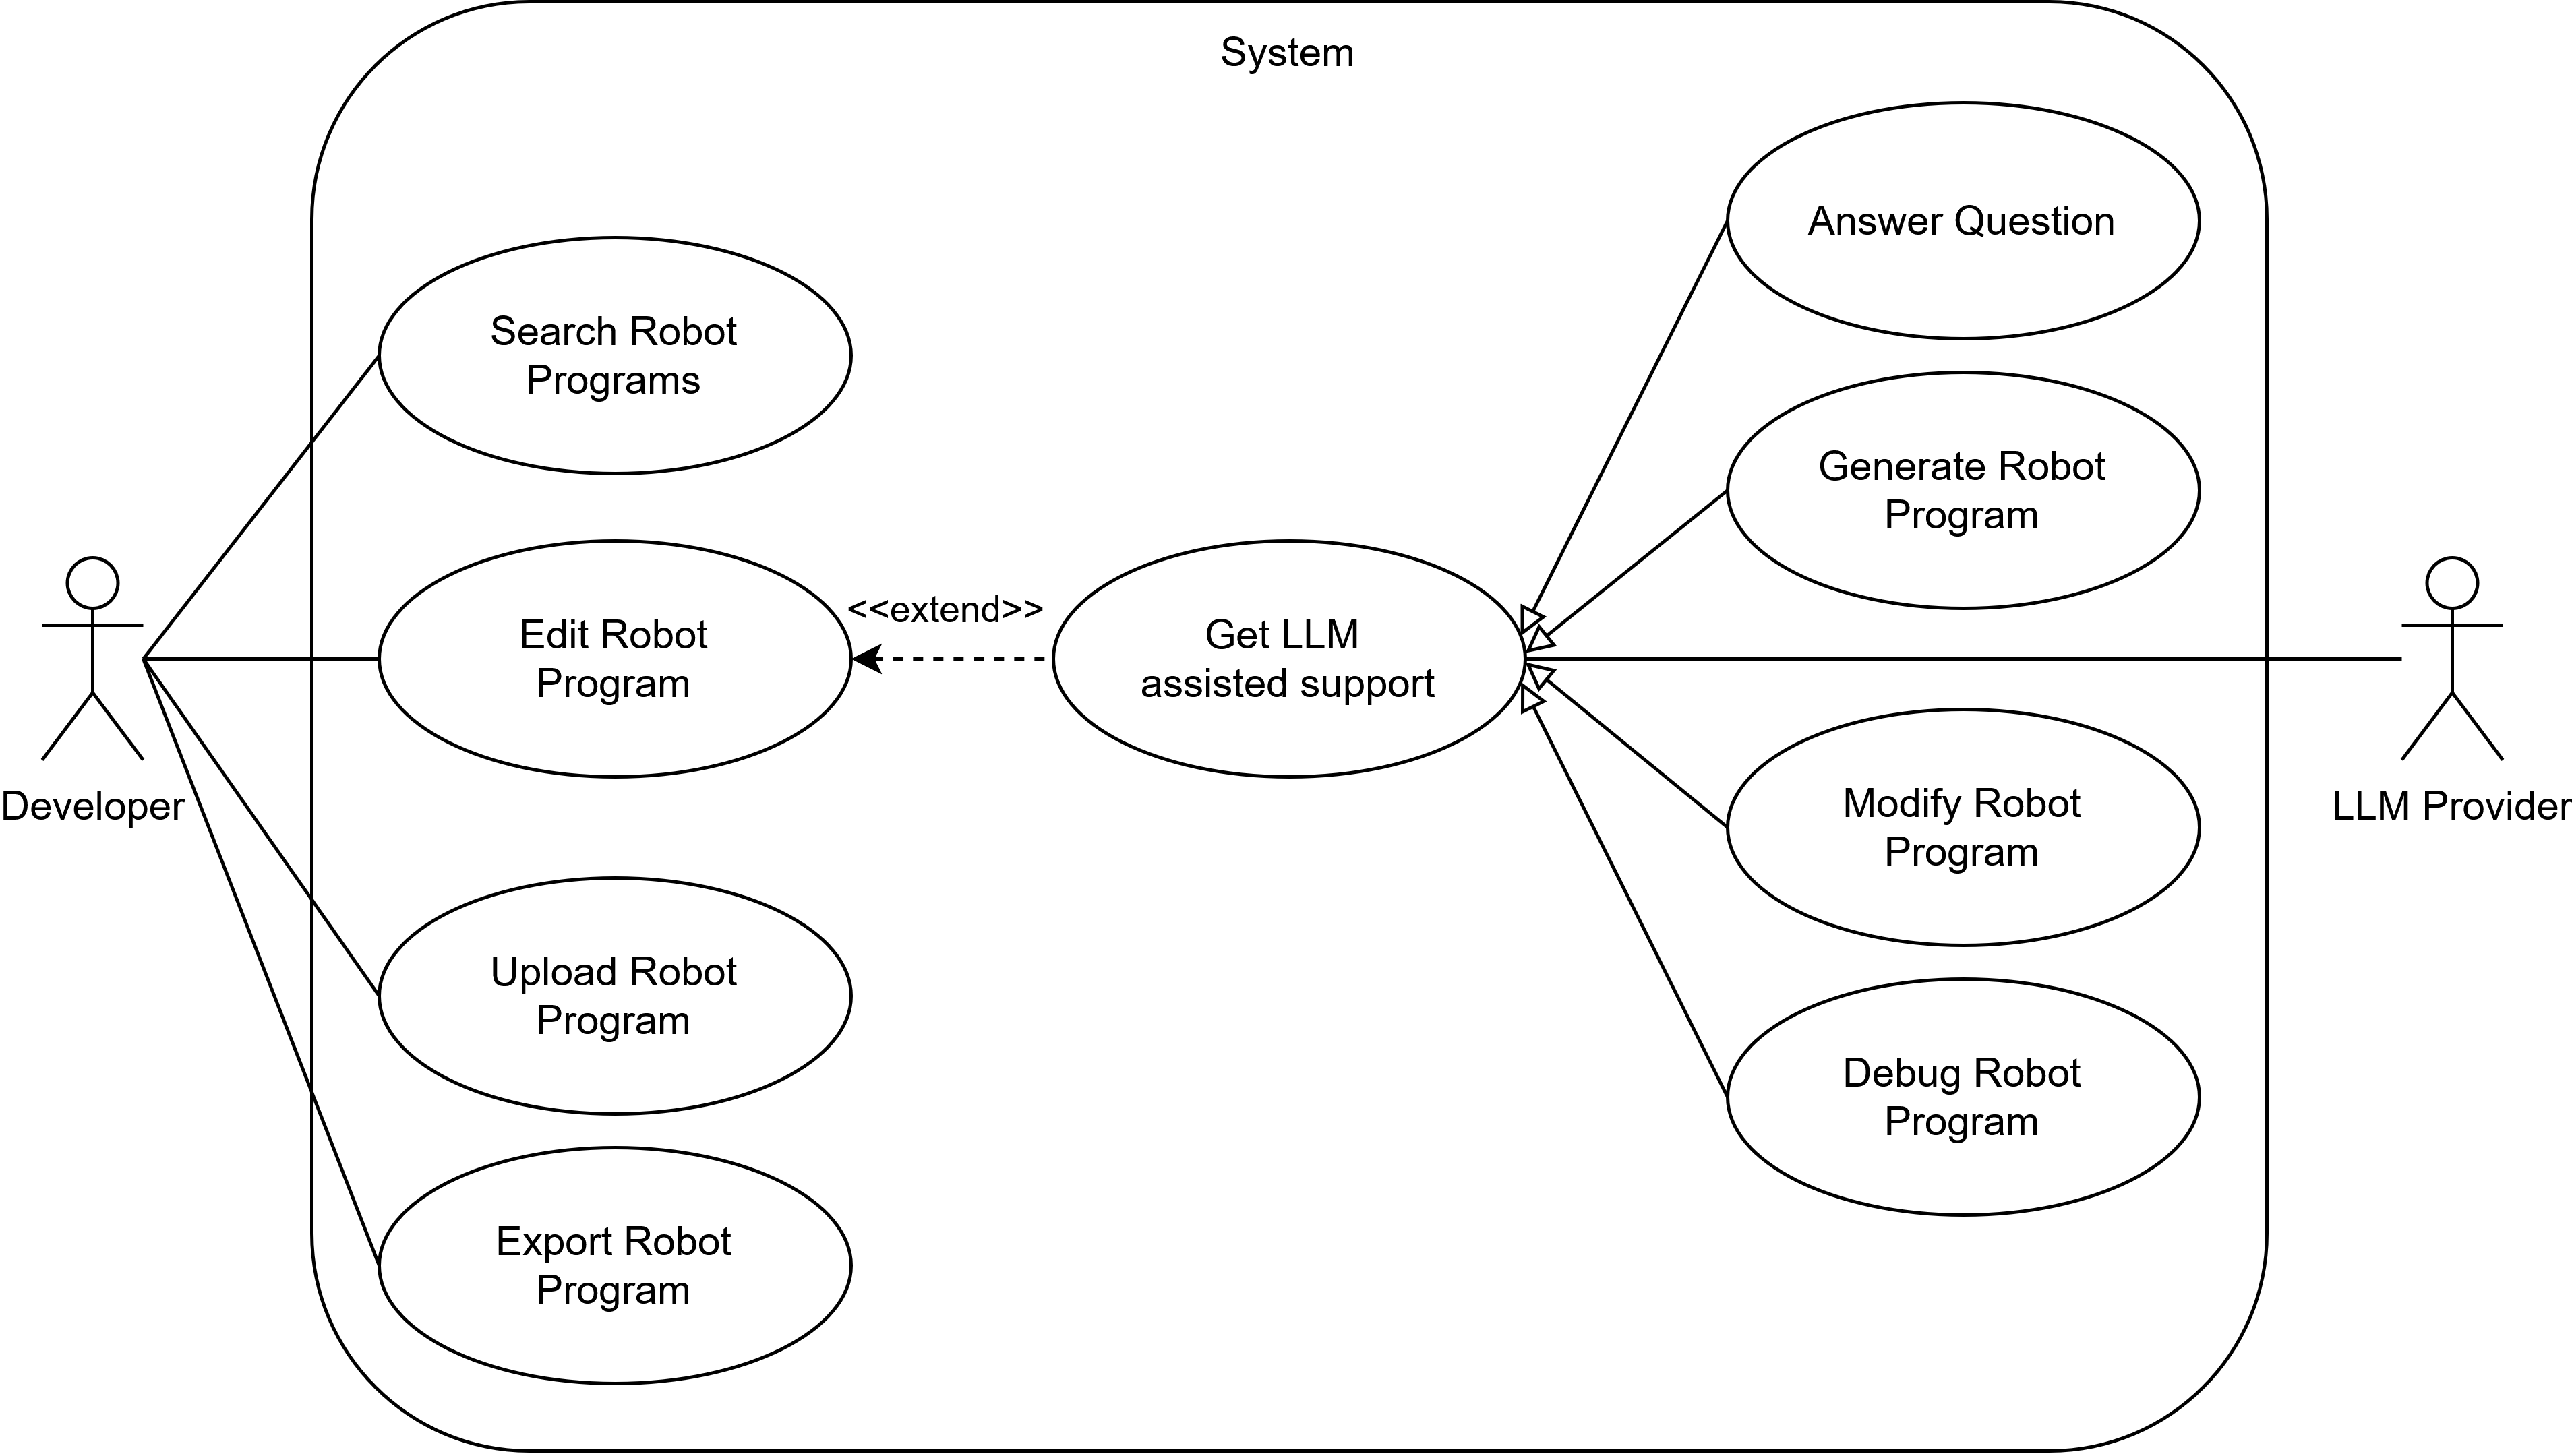
\includegraphics[width=\columnwidth]{media/use-case-diagram.png}
    \caption{{Use Case Diagram.}}
    \label{fig:requirement-engineering:use-case-diagram}
\end{figure}


\section{Requirements Specification} \label{sec:requirement_engineering:specification}
The final set of functional and non-functional requirements is specified below.

\textbf{Functional Requirements (FR):}
\begin{adjustwidth}{\indentWidthTwenty}{\indentWidthTwenty}
    \textit{\textbf{System:}}
\end{adjustwidth}
\begin{adjustwidth}{\indentWidthForty}{\indentWidthForty}
    \textit{\textbf{FR1:} The system shall allow searching for robot programs to identify programs for future development.}
\end{adjustwidth}
\begin{adjustwidth}{\indentWidthForty}{\indentWidthForty}
    \textit{\textbf{FR2:} The system shall allow for uploading robotic programs for inclusion in the program repository and identification in future queries.}
\end{adjustwidth}
\begin{adjustwidth}{\indentWidthForty}{\indentWidthForty}
    \textit{\textbf{FR3:} The system shall allow for exporting robot programs.}
\end{adjustwidth}
\begin{adjustwidth}{\indentWidthForty}{\indentWidthForty}
    \textit{\textbf{FR4:} The system shall provide a robot program editor.}
\end{adjustwidth}
\begin{adjustwidth}{\indentWidthForty}{\indentWidthForty}
    \textit{\textbf{FR5:} The system shall provide LLM-assisted support by answering user queries expressed in natural language.}
\end{adjustwidth}

\begin{adjustwidth}{\indentWidthTwenty}{\indentWidthTwenty}
    \textit{\textbf{AI Assistant:}}
\end{adjustwidth}
\begin{adjustwidth}{\indentWidthForty}{\indentWidthForty}
    \textit{\textbf{FR6:} The AI assistant responses shall be human-readable.}
\end{adjustwidth}
\begin{adjustwidth}{\indentWidthForty}{\indentWidthForty}
    \textit{\textbf{FR7:} The AI assistant shall support the user in comprehending robotic programs by answering user questions.}
\end{adjustwidth}
\begin{adjustwidth}{\indentWidthForty}{\indentWidthForty}
    \textit{\textbf{FR8:} The AI assistant shall support modification tasks by suggesting changes to existing robot programs based on user instructions.}
\end{adjustwidth}
\begin{adjustwidth}{\indentWidthForty}{\indentWidthForty}
    \textit{\textbf{FR9:} The AI assistant shall retain relevant conversational context within a session to support follow-up questions.}
\end{adjustwidth}
\begin{adjustwidth}{\indentWidthForty}{\indentWidthForty}
    \textit{\textbf{FR10:} The AI assistant shall indicate uncertainty when the available information is insufficient to provide a reliable answer.}
\end{adjustwidth}


\textbf{Non-Functional Requirements (NFR):}
\begin{adjustwidth}{\indentWidthTwenty}{\indentWidthTwenty}
    \textit{\textbf{Performance:}}
\end{adjustwidth}
\begin{adjustwidth}{\indentWidthForty}{\indentWidthForty}
    \textit{\textbf{NFR1:} The system shall provide responses to user queries within 10 seconds.}
\end{adjustwidth}

\begin{adjustwidth}{\indentWidthTwenty}{\indentWidthTwenty}
    \textbf{Modifiability:}
\end{adjustwidth}
\begin{adjustwidth}{\indentWidthForty}{\indentWidthForty}
    \textit{\textbf{NFR2:} LLM-specific functionality shall be isolated from core system components to enable integration of alternative language models with minimal implementation effort.}
\end{adjustwidth}

\begin{adjustwidth}{\indentWidthTwenty}{\indentWidthTwenty}
    \textbf{Observability:}
\end{adjustwidth}
\begin{adjustwidth}{\indentWidthForty}{\indentWidthForty}
    \textit{\textbf{NFR3:} The system shall log all LLM interactions, including user inputs, generated outputs, timestamps, and request identifiers, to support monitoring, debugging, and traceability.}
\end{adjustwidth}

\begin{adjustwidth}{\indentWidthTwenty}{\indentWidthTwenty}
    \textbf{Traceability:}
\end{adjustwidth}
\begin{adjustwidth}{\indentWidthForty}{\indentWidthForty}
    \textit{\textbf{NFR4:} For all responses generated using retrieval-augmented generation (RAG), the system shall expose the references of the retrieved source documents used during response generation.}
\end{adjustwidth}

\begin{adjustwidth}{\indentWidthTwenty}{\indentWidthTwenty}
    \textit{\textbf{Usability:}}
\end{adjustwidth}
\begin{adjustwidth}{\indentWidthForty}{\indentWidthForty}
    \textit{\textbf{NFR5:} A majority of users shall rate the LLM-supported responses as clear and understandable.}
\end{adjustwidth}
\begin{adjustwidth}{\indentWidthForty}{\indentWidthForty}
    \textit{\textbf{NFR6:} A majority of users shall rate the system as useful for comprehending robotic programs.}
\end{adjustwidth}
\begin{adjustwidth}{\indentWidthForty}{\indentWidthForty}
    \textit{\textbf{NFR7:} A majority of users shall rate the system as useful for modifying robotic programs.}
\end{adjustwidth}
\begin{adjustwidth}{\indentWidthForty}{\indentWidthForty}
    \textit{\textbf{NFR8:} A majority of users shall rate the LLM-supported responses as relevant to the user query.}
\end{adjustwidth}
\begin{adjustwidth}{\indentWidthForty}{\indentWidthForty}
    \textit{\textbf{NFR9:} A majority of users shall rate the LLM-supported responses as factually correct.}
\end{adjustwidth}
\chapter{Design} \label{chapter:design}
This chapter presents the design process for the system, including architectural choices and the rationale behind them. The design is guided by the requirements from the previous chapter.


\section{Design Context}
This project is based on two primary data sources: robotic programs developed for Universal Robots systems and technical documentation from the robot manufacturer. These data sources represent both concrete implementations of robotic tasks and contextual knowledge about robot capabilities and programming concepts.

\subsection{Robot Programs}
The robotic programs, in the Universal Robots \texttt{.urpx} format, represents a complete robot program. Internally, these files follow a structured, hierarchical format that resembles JSON. The structured nature of the \texttt{.urpx} files allows for systematic extraction of metadata describing the semantics of the program. For this theis, it is assumed that every program file is associated with a metadata file that characterizes the program. A similar metadata file is eventually expected to be available from the FERA program repository as well. This metadata includes attributes such as the application type, actions performed, and the hardware context e.g., robot model and end-effector type.

The following (see Code~\ref{listing:design:data_robot_programs}) shows the JSON structure of the program metadata.
\begin{listing}[h]
    \begin{minted}{json}
                            {
                                "id": "integer",
                                "name": "string",
                                "robotType": "string",
                                "applicationType": "string",
                                "gripperType": ["string"],
                                "image": "string",
                                "dataAvailable": "string",
                                "components": "string",
                                "program": "string",
                                "additionalImage": "string",
                                "totalRating": "integer",
                                "ratingCount": "integer",
                                "objectType": ["string"],
                                "objectWeight": "number",
                                "cncDoorControl": "boolean",
                                "communicationType": "string",
                                "actions": ["string"]
                            }
    \end{minted}
    \caption{JSON structure of robotic program metadata.}
    \label{listing:design:data_robot_programs}
\end{listing}

\subsection{Robot Documentation}
In addition to program data, technical documentation is available in \texttt{.pdf} format. This documentation includes manuals, guidelines, and reference materials from the Universal Robots documentation portal. \cite{UniversalRobots2026Downloads} Each documentation file contains upward of hundreds of pages of information. Unlike robotic programs, which are structured artifacts, documentation represents unstructured textual data that provides explanatory and contextual information about robot functionality and programming concepts.


\newpage
\section{Architectural Design}
As presented in Chapter~\ref{chapter:related-work}, recent advances in LLMs and AI assistants have demonstrated strong potential within software engineering, where they are increasingly used for tasks such as code generation, question answering, debugging, and code modification. We explore how similar assistant-based approaches can support robotic program development.

The functional requirements (see Section~\ref{sec:requirement_engineering:specification}) of the system specify capabilities beyond standalone language generation. Tasks such as answering questions about robotic programs, generating or modifying code, and debugging robot programs require the assistant to have agentic capabilities to efficiently support the developer. For example, answering a question about a robotic program may require grounding the response in relevant documentation. Modifying a robot program may require inspecting the program and understanding the existing code, iteratively refining the modification based on feedback, and validating the modified program.

Consequently, the assistant should be augmented with a set of tools that enable these functional requirements. Rather than acting only as a static response generator, it should support an interactive workflow in which external tools can be used whenever a user query requires it.

The assistant would ideally have access to multiple categories of tools that support different stages of the robotic program development workflow. Retrieval tools would enable access to technical documentation and previously developed robotic programs relevant to the user's query. Program inspection tools would allow the assistant to analyze program structure, metadata, and control flow directly from the underlying robotic artifacts, enabling reasoning grounded in the program itself rather. Modification tools would support structured editing and transformation of programs. Verification tools, including syntax checkers, schema validators, and static analysis utilities, would support validation of generated modifications. Simulation tools could enable evaluation of generated changes against expected robot behavior in controlled environments prior to execution on physical systems. Collectively, these tool categories support the broader development workflow of retrieval, comprehension, modification, verification, and validation of robotic programs.

However, use of such tools depends on the user query and requires an architecture that supports agentic behavior. The assistant must be able to decide when to use tools, which tools to use, and how to integrate tool output into its reasoning and response generation. Thus, the assistant architecture adopted in this project is inspired by the ReAct framework (also mentioned in Chapter~\ref{chapter:related-work}), in which a language model iteratively alternates between reasoning about a task and invoking external tools to gather information or perform actions. This approach is well suited for robotic program development tasks because user requests may require multiple intermediate steps before a suitable response can be generated.

Figure \ref{fig:design:agentic_orchestration_flowchart} shows the agentic orchestration loop architecture and illustrates how reasoning, tool use, evidence evaluation, and response synthesis are connected.

\begin{figure}[H]
    \centering
    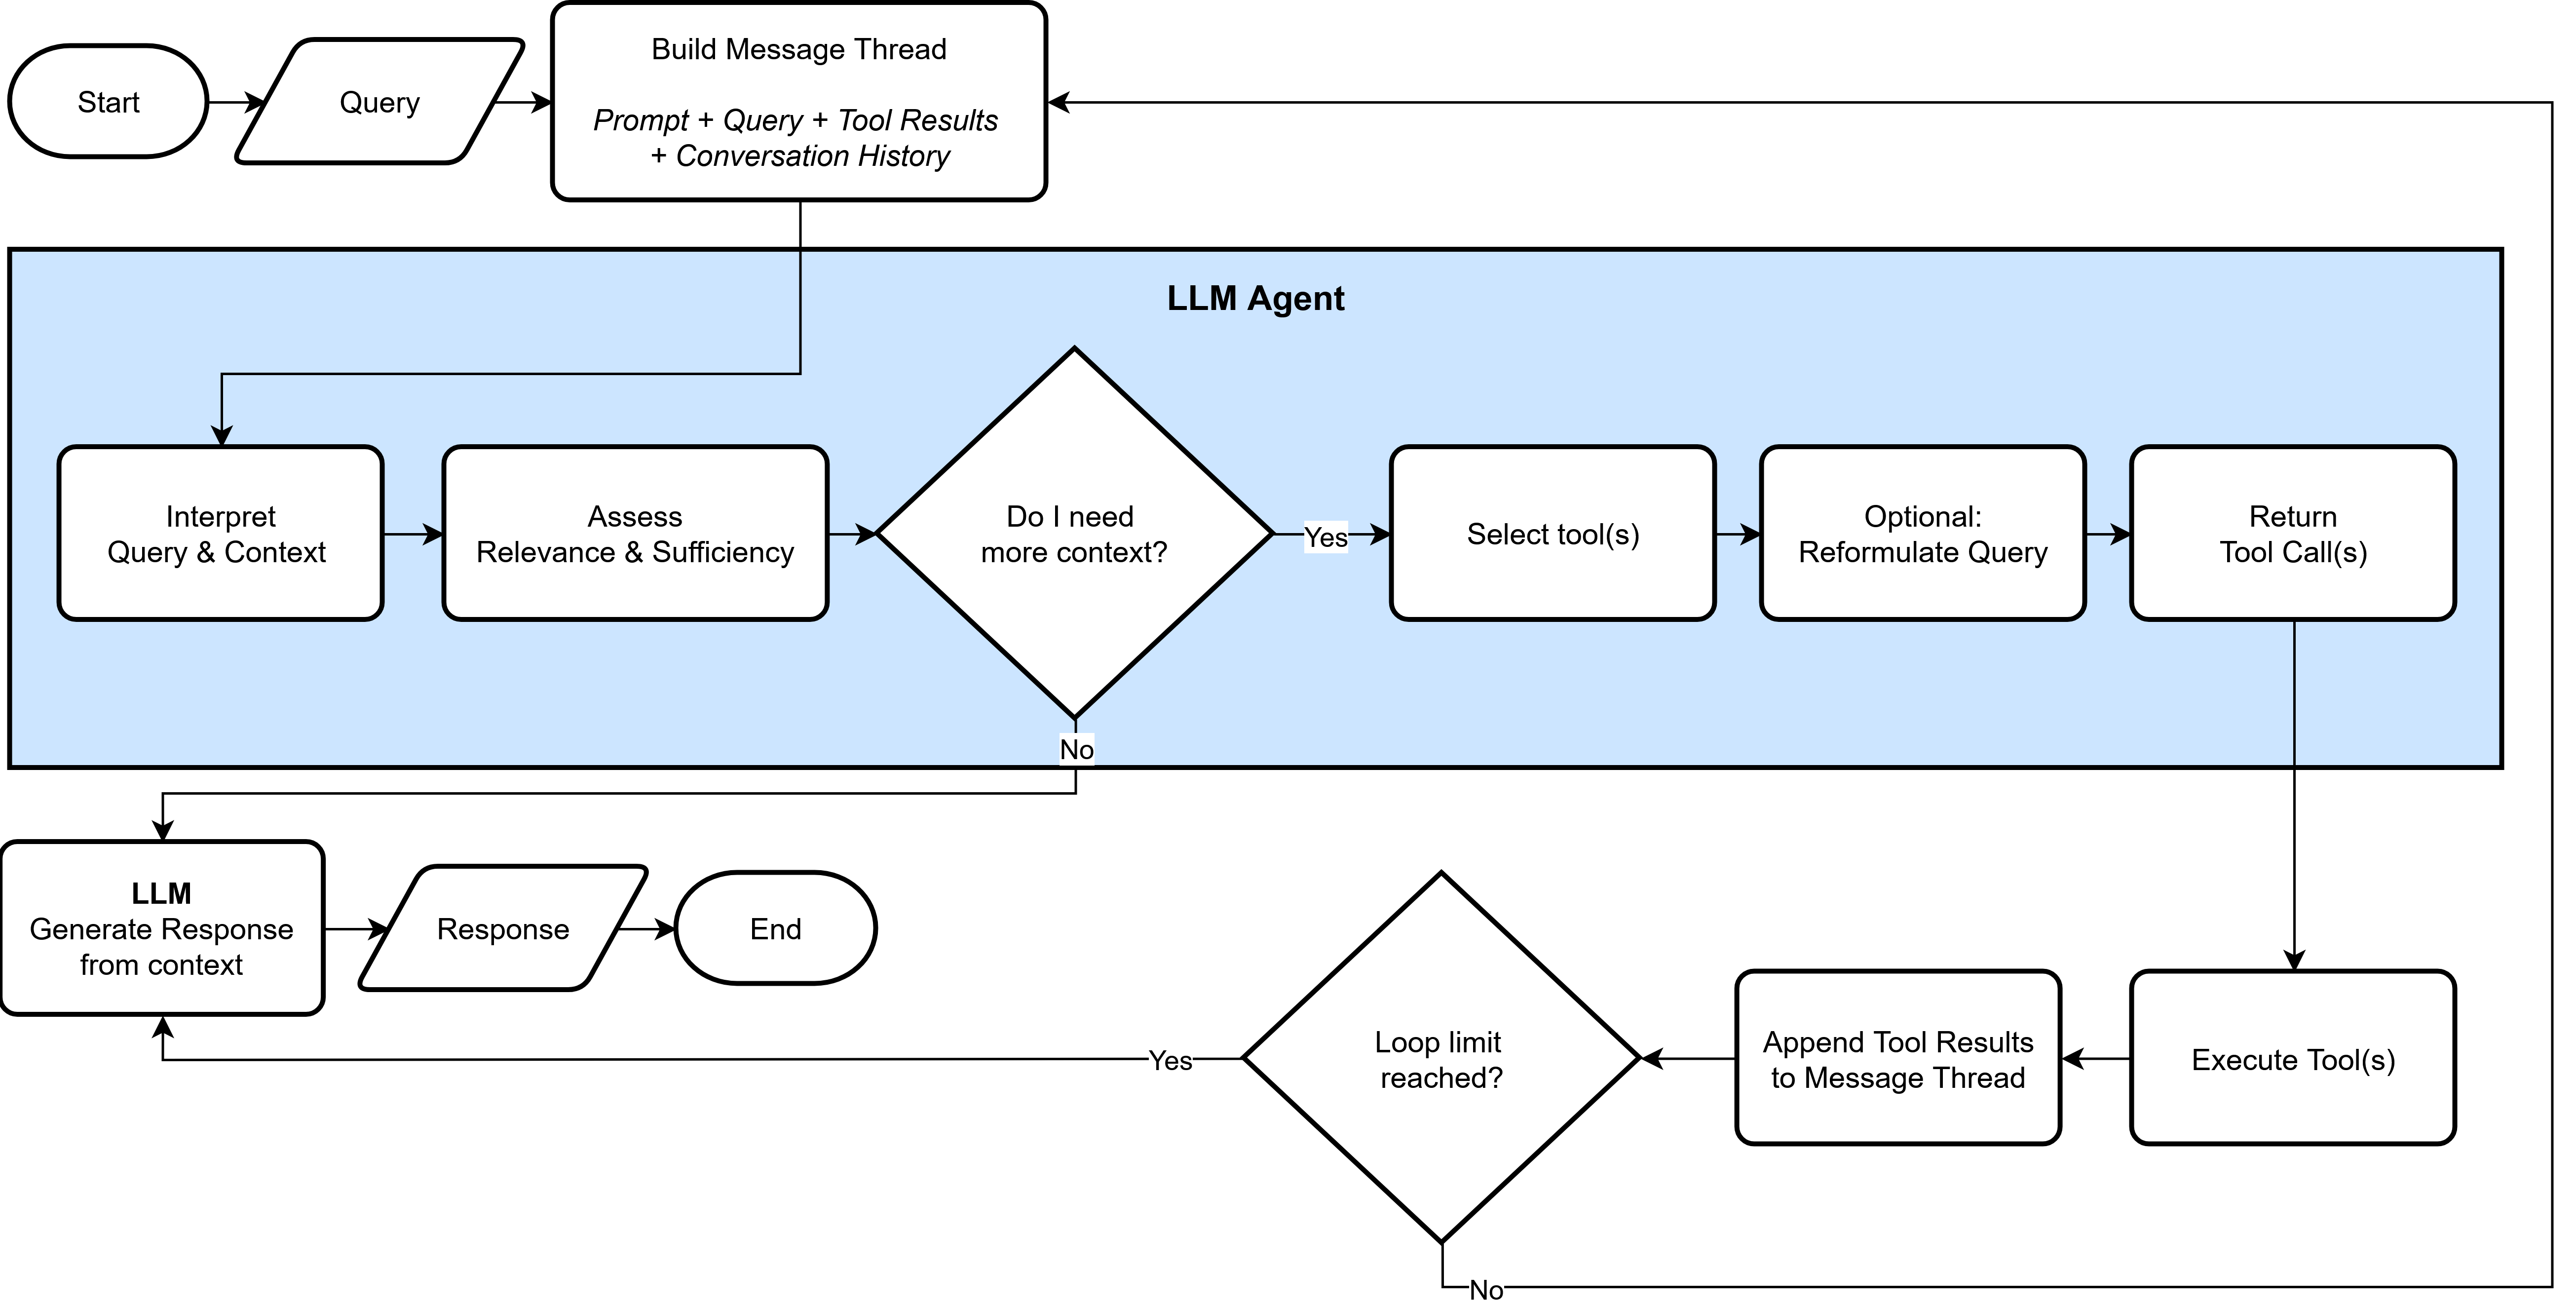
\includegraphics[width=\columnwidth]{media/orchestration-flowchart.png}
    \caption{{Agentic orchestration loop flowchart.}}
    \label{fig:design:agentic_orchestration_flowchart}
\end{figure}

Within this architecture, a language model acts as the orchestration component responsible for interpreting user requests, selecting appropriate tools, reasoning over retrieved information and generating responses. Having multiple specialized LLMs for different roles e.g., one for orchestration and another for response generation, could result in better performance and quality because each model can be optimized for its specific purpose. However, to take full advantage of this, we would have to train or fine-tuning domain-specific models, which is not feasible given the scope of the project and the available data. Therefore, the design of the system should for now use general-purpose LLMs for both orchestration and response generation, and the focus should be on augmenting these models with the necessary tools and retrieval capabilities to support robotic program development tasks. This design allows the system to leverage the general reasoning and language capabilities of existing LLMs, while future work can explore the potential benefits of domain-specific training or fine-tuning for improved performance in robotic programming contexts.

Due to the scope of this thesis, the following system design focuses primarily on retrieval-based tools for integrating the available robotic knowledge sources into the assistant's reasoning process. Additional tools are discussed as directions for future work in Chapter~\ref{sec:discussion:future-work}.


\newpage
\section{Retrieval-Augmented Generation (RAG)}
As discussed in Section~\ref{sec:related-work:RAG}, retrieval-augmented generation extends a language model with access to external knowledge. This allows the integration of the robotic domain knowledge into the general language model to ground its responses in up-to-date and relevant information, without requiring the model itself to be retrained whenever the knowledge base changes. It also supports transparency, because retrieved context can be traced back to its source.

Figure~\ref{fig:design:rag} illustrates this overall retrieval-augmented generation pattern, in which external knowledge is retrieved and incorporated into the model context before response synthesis.

\begin{figure}[H]
    \centering
    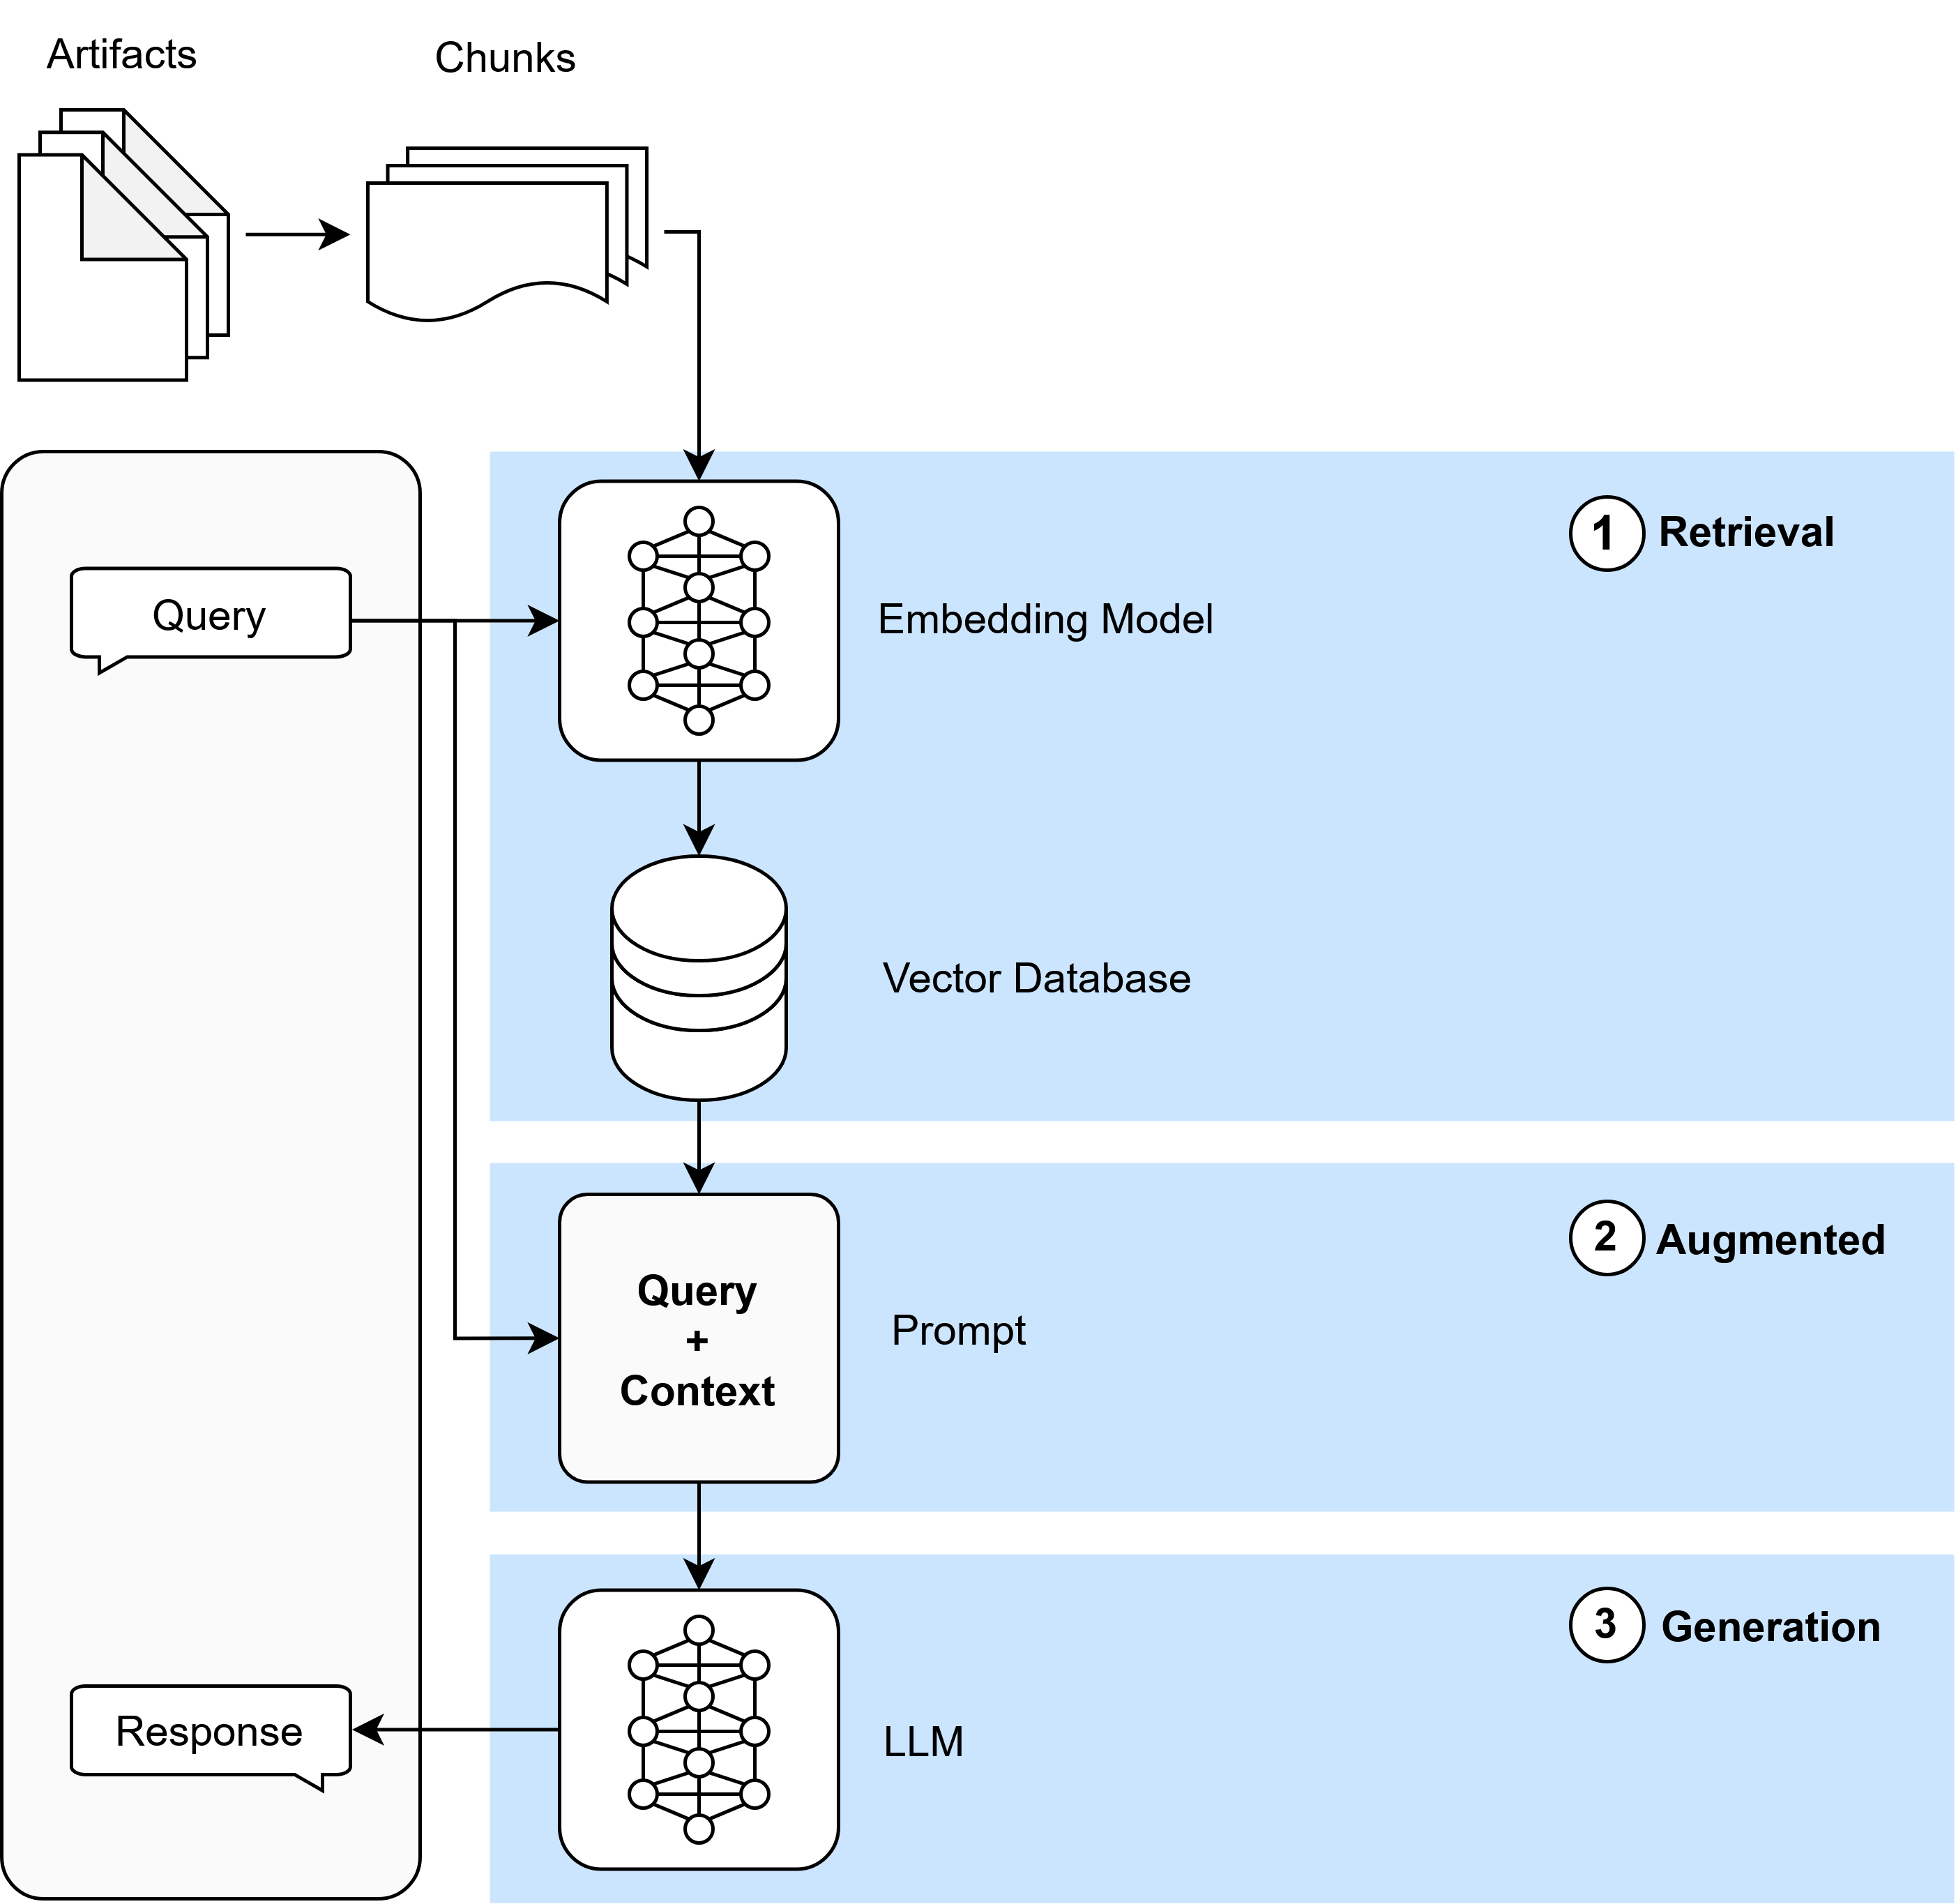
\includegraphics[width=0.8\columnwidth]{media/rag.png}
    \caption{{Retrieval-Augmented Generation (RAG).}}
    \label{fig:design:rag}
\end{figure}


In Section~\ref{sec:related-work:RAG}, several RAG variants were presented, naive RAG, advanced RAG, modular RAG, and agentic RAG. Agentic RAG overlaps with the ReAct-style agentic orchestration loop described above, as both emphasize the role of retrieval as an explicit tool-mediated action within the reasoning loop. This design allows the assistant to adaptively decide when and how to retrieve evidence based on the evolving context of the interaction, rather than relying on a fixed retrieval step before response generation. The overlap means that providing the orchestration agent with retrieval tools effectively implements an agentic RAG architecture, where retrieval is integrated into the assistant's reasoning process in a flexible and context-sensitive way.

\subsection{Retrieval}
The retrieval mechanism is designed around semantic search, in which user queries and indexed artifacts are represented in a shared semantic space. Rather than depending solely on exact keyword overlap, the system can identify programs and documentation passages whose meaning is close to the user's intent. This is well suited to the present domain because users formulate requests in natural language, whereas the underlying sources contain robotics-specific terminology, structured metadata, and implementation details that may not share the same vocabulary.

Alternative strategies were considered. Exact keyword search is effective when the user's terminology closely matches the corpus, but it performs poorly when the same concept is expressed using different words. However, hybrid retrieval, combining semantic similarity with keyword constraints, remains a relevant extension for cases where exact identifiers or parameter names are important.

Figure \ref{fig:design:semantic_search} illustrates the semantic search approach adopted in the system.

\begin{figure}[H]
    \centering
    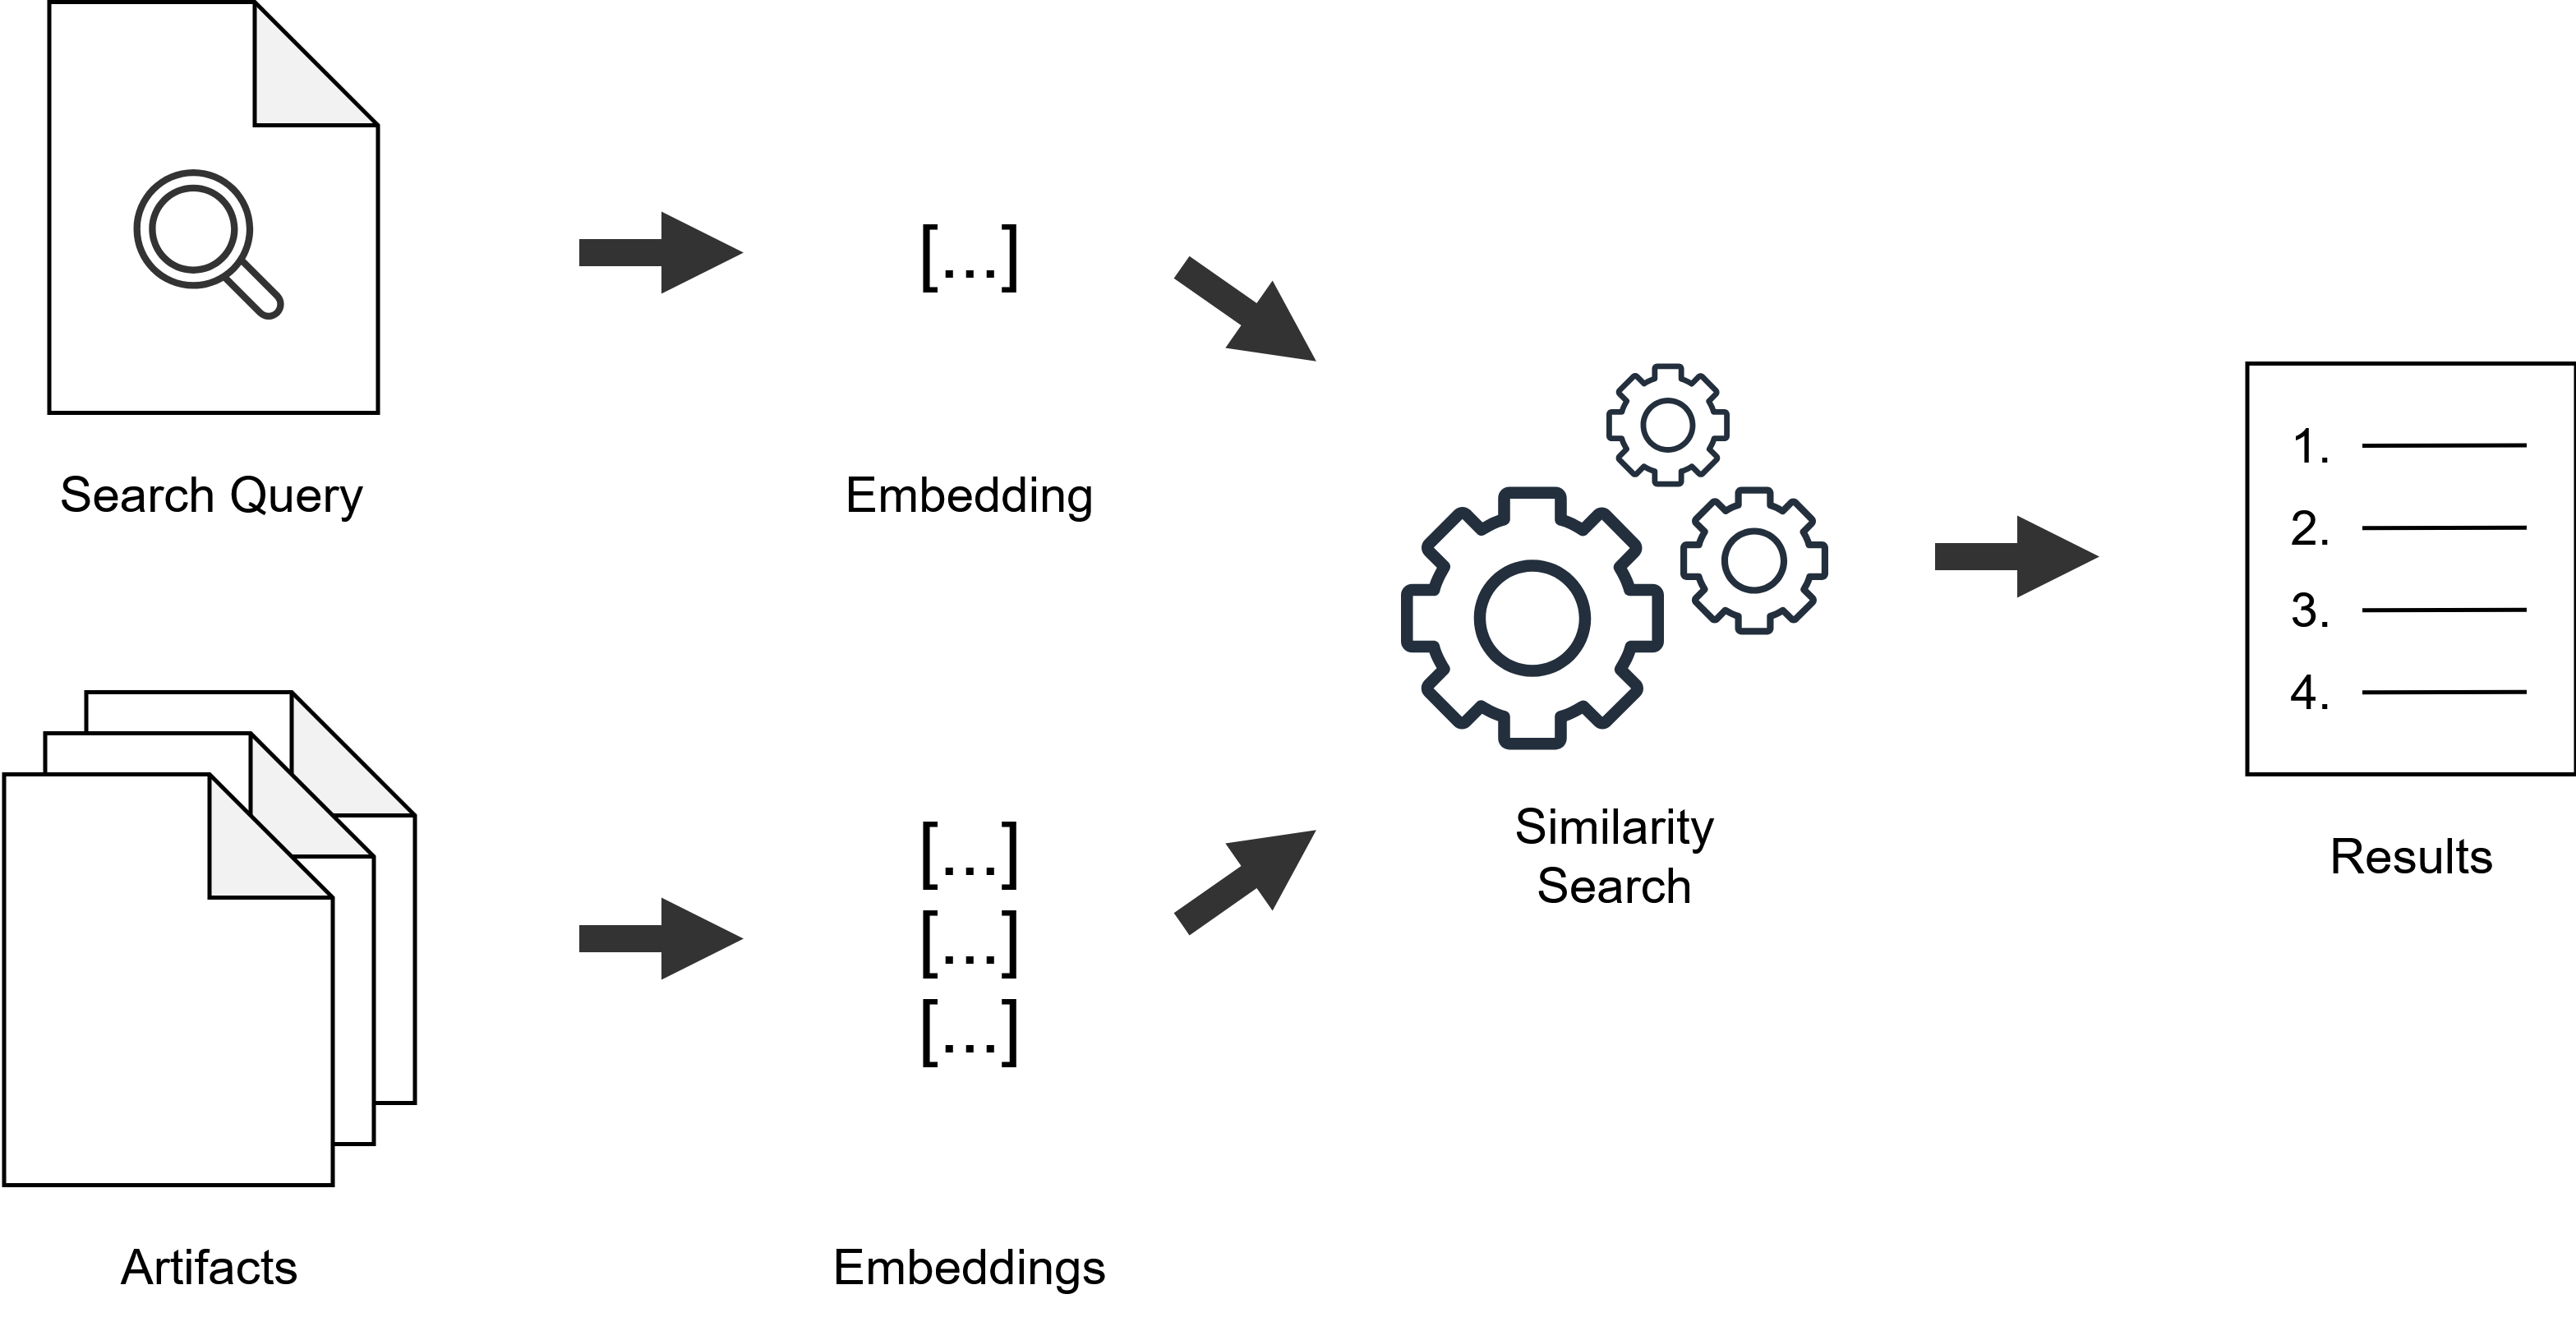
\includegraphics[width=0.8\columnwidth]{media/semantic_search.png}
    \caption{{Semantic Search.}}
    \label{fig:design:semantic_search}
\end{figure}


\subsection{Data Pipeline}
RAG depends on external knowledge being available in a form that can be retrieved efficiently at runtime. In this thesis, those knowledge sources are program metadata, robot program code, and documentation. The data pipeline should therefore convert these raw sources into retrieval-oriented representations, embed those representations, and organize them in a way that supports efficient semantic search. The quality of this pipeline directly affects how well the assistant can identify and use relevant sources during interaction.

These data sources should be preserved as separate representations, opposed to being merged into a single undifferentiated retrieval space, because they serve different roles in the assistant workflow. Metadata-oriented program summaries support discovery of relevant examples, program-code chunks provide structural detail for comprehension and modification tasks, and documentation chunks contribute explanatory knowledge. Keeping these sources separate improves retrieval controllability and makes it easier to combine evidence deliberately during response generation.

The data pipeline should operate as an offline preparation layer so that computationally expensive transformation, chunking, and embedding operations do not have to be performed during user interaction. This improves runtime responsiveness and preserves modularity, since chunking strategies, embedding models, and ingestion processes can be refined independently of the assistant's orchestration logic.

Figure \ref{fig:design:data_ingestion} illustrates the data pipeline, which consists of three stages: data transformation, embedding, and ingestion, each discussed in the subsequent subsections.

\begin{figure}[H]
    \centering
    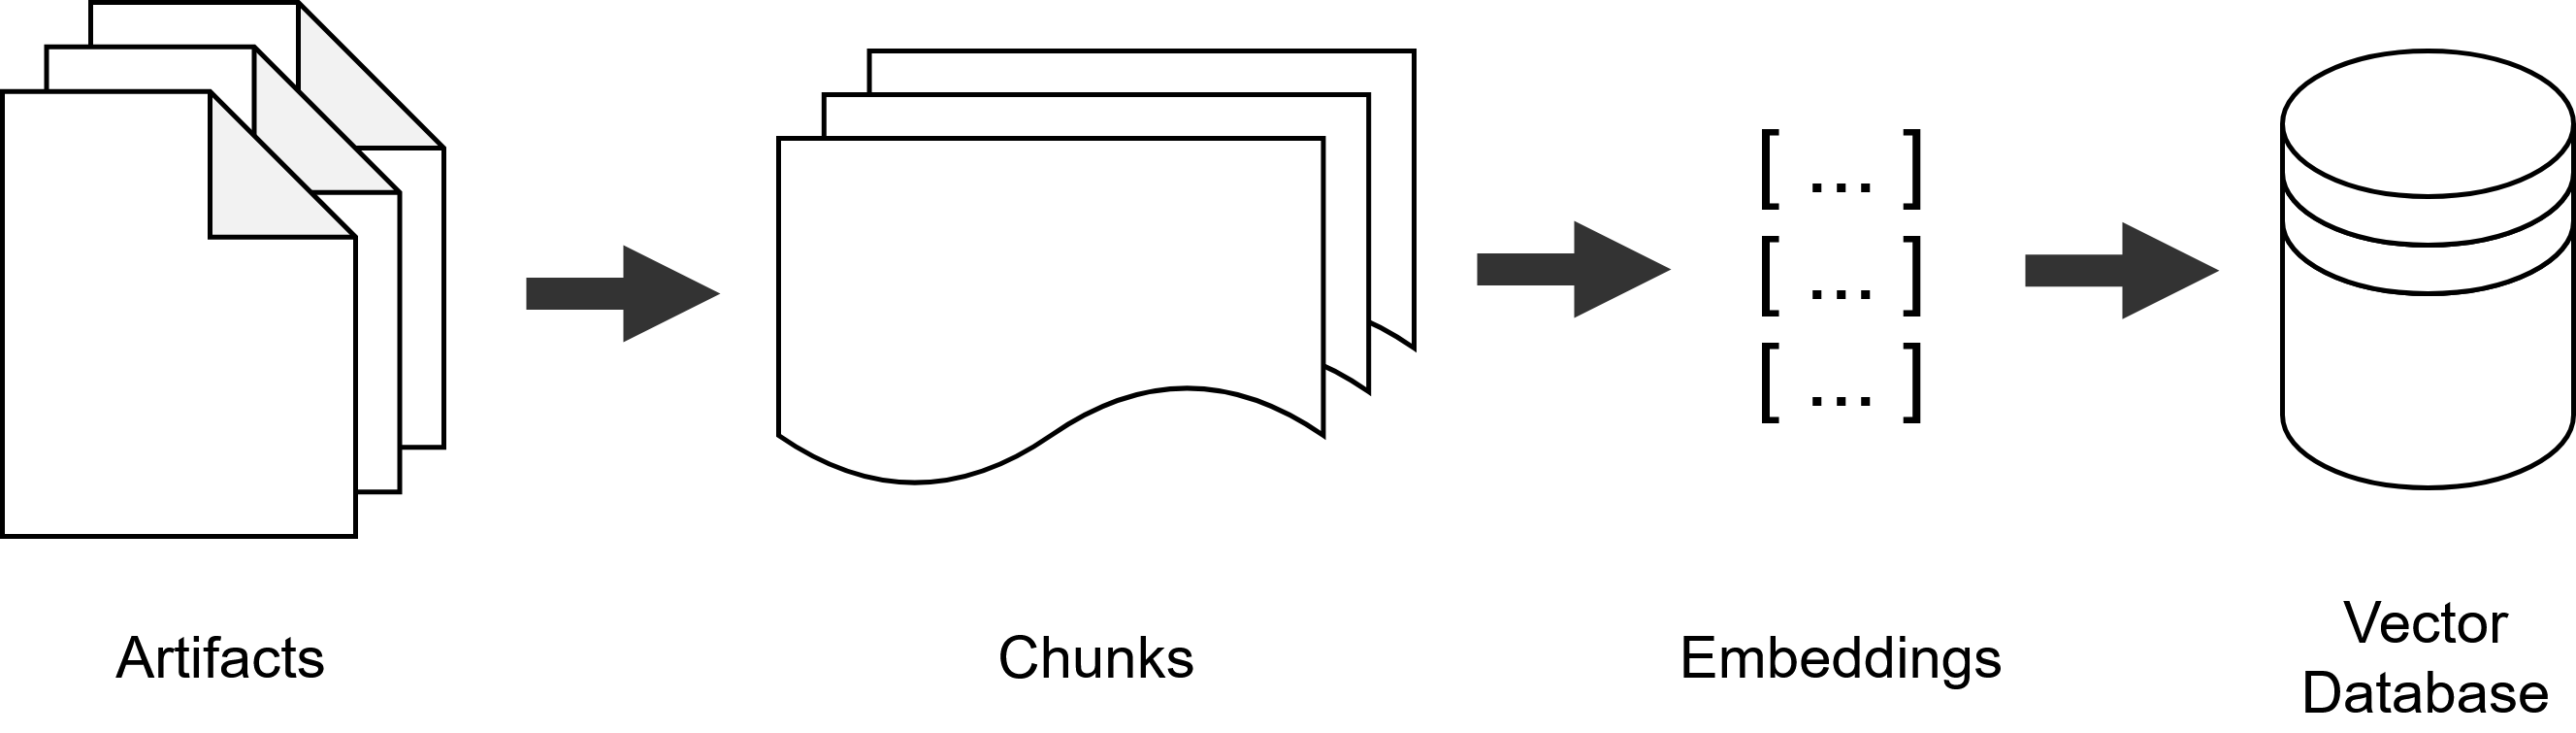
\includegraphics[width=0.9\columnwidth]{media/data_ingestion.png}
    \caption{{Data Pipeline.}}
    \label{fig:design:data_ingestion}
\end{figure}

\subsubsection{Transformation and Chunking}
The system relies on three information sources with different semantic roles. Because these sources differ in structure and purpose, transformation and chunking are designed per source. A critical constraint is the limited context window of language models: entire programs or documentation files quickly exhaust available model context, making it impractical to retrieve full artifacts for synthesis. Chunking is therefore essential to partition large artifacts into focused units that can fit within context limits while preserving semantic coherence. This introduces a design trade-off: finer-grained chunking can improve retrieval precision, but it may fragment context across multiple chunks, whereas coarser chunking preserves more local context at the cost of lower retrieval precision and more irrelevant surrounding material. Additionally, model performance can degrade as the context window fills, making efficient use of limited context, as well as context management, important design concerns. \cite{liu2024lost}

\paragraph{Program Metadata}~\\
Program metadata captures high-level intent, including task type, robot context, components, and actions. During transformation, these structured fields should be converted into concise natural-language representations to align with the behavior of semantic search and embedding models, which generally capture meaning more effectively from textual descriptions than from raw structured syntax. While JSON structures could be embedded directly, this would increase token usage without adding comparable semantic value for retrieval. Metadata-oriented representations are therefore designed for intent-level retrieval, either for identifying programs or for guiding the assistant in reasoning about high-level implementation details.

\paragraph{Program Code}~\\
Program code provides structural details that metadata alone cannot express. The program structures should be transformed into semantically meaningful fragments. As with metadata, structured content is expressed as compact natural-language descriptions, because dense structural encodings increase token volume but often contribute less semantic signal for embedding-based retrieval. Chunking at this level balances precision: shorter chunks enable targeted retrieval of specific operations or patterns, but longer chunks preserve more operational context, which may be needed for modification tasks. The chunking strategy should use structural cues such as node definitions to create coherent units that can be retrieved and reasoned about effectively. This allows the assistant to access relevant code details without overwhelming the model with excessive context.

\paragraph{Documentation}~\\
Documentation is an unstructured source composed of long, multi-topic texts. It should therefore be segmented into coherent chunks that align with local concepts and preserve contextual continuity. A key design consideration for documentation chunking is overlap: adjacent chunks should be permitted to share boundary content (typically a few sentences) so that retrieval at a chunk boundary does not abruptly lose context needed for the synthesis model to reason about the retrieved passage. This sliding-window approach is particularly important for documentation because technical concepts often span multiple sentences, and a sharp chunk boundary can cut sentences short. Chunk boundaries are aligned with structural features, section headers, paragraphs, and topic shifts, rather than fixed token counts, which better preserves semantic coherence. This enables targeted retrieval of relevant explanatory passages instead of entire manuals, which improves precision for technical questions. Less relevant sections e.g. table of contents should be filtered out during transformation to avoid polluting the retrieval space with low-value content.

\subsubsection{Embedding}
Following transformation and chunking, the resulting program representations and documentation chunks should be embedded into dense vector representations to enable semantic similarity search. Embedding the transformed natural-language representations allows user queries to be matched against robotic programs and documentation based on semantic meaning.

\subsubsection{Ingestion}
Ingestion is the final preparation stage in which the embedded representations are written into the retrieval layer together with the metadata needed to use them effectively at runtime The ingestion design decides how the assistant's knowledge is organized and exposed to retrieval, and therefore determines which kinds of evidence can be retrieved, how they are distinguished from one another, and how they can later be traced back to their sources.

The system should preserve the three evidence types as separate representations: metadata representations, code-level program chunks, and documentation chunks. This separation reflects their different roles in the assistant workflow. Metadata-oriented program representations support retrieval of relevant robotic solutions at the task level, program-code chunks provide structural detail for comprehension and modification, and documentation chunks contribute explanatory knowledge. Keeping these representations separate improves retrieval control.

Ingestion should also preserve provenance. Each ingested entry should retain source identity and linking information to the underlying artifact from which it was derived. This is particularly important for robotic programs and metadata, where the semantic representations are useful for retrieval, but the original structured artifacts are required during reasoning and response generation. This also allows the assistant to trace retrieved evidence back to its source, which supports transparency and enables the user to inspect the original artifact when needed.


\section{Frontend}
\subsection{User Interface}
The user interface forms the primary interaction point between the developer and the assistant, and its design therefore plays an important role in how effectively the assistant can support robotic program development tasks. The interface should expose the assistant's capabilities in a way that supports both exploration of existing robotic solutions and focused comprehension and modification of individual programs.

These activities place different demands on the interface and should therefore be separated into distinct workspaces. Search-oriented workflows benefit from lightweight navigation across many candidate programs, whereas comprehension and modification tasks require sustained attention to a single artifact together with supporting contextual information. The frontend design therefore separates interaction into a search workspace and an editor workspace.

A web-based frontend was selected to align with both the expected FERA platform architecture and modern robotics software environments such as PolyScope X, which are themselves web-oriented. Since the assistant is intended to support workflows within these environments, adopting a compatible frontend architecture simplifies potential integration and promotes consistency across systems. In addition, web applications are platform-independent and support distributed system architectures in which frontend, backend, retrieval infrastructure, and language-model orchestration remain separated components communicating through network interfaces. Modern web technologies are also well suited for AI-assisted interaction patterns, including conversational interfaces, asynchronous communication, and streaming responses.

Figures~\ref{fig:design:lofi_search} and \ref{fig:design:lofi_edit} present low-fidelity wireframes for the two workspaces. The search workspace shown in Figure~\ref{fig:design:lofi_search} prioritizes natural-language querying and inspection of ranked program results. Users should be able to compare candidate programs based on semantic descriptions and metadata before loading a specific artifact into the editor workspace. This supports efficient discovery of relevant robotic solutions.

\begin{figure}[H]
    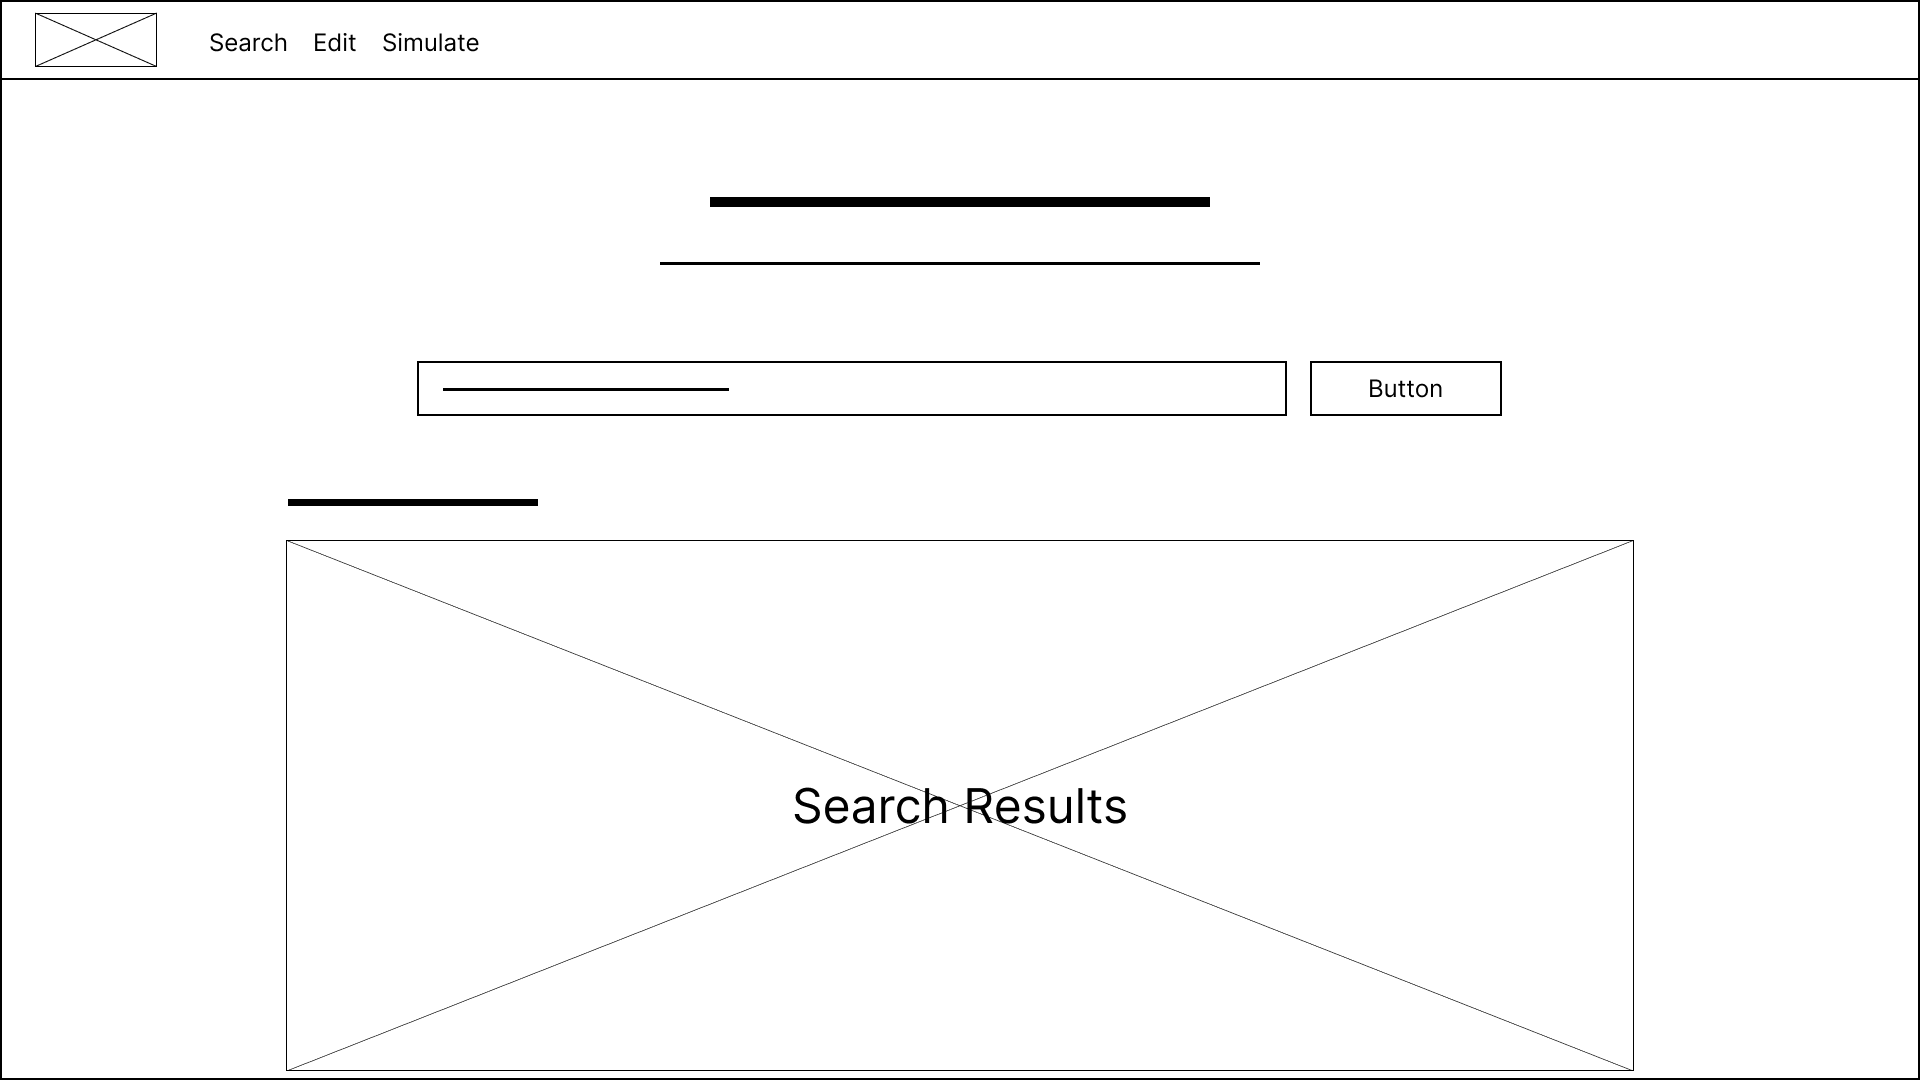
\includegraphics[width=\columnwidth]{media/lofi-search-tab.png}
    \caption{{Low-fidelity wireframe of the search interface.}}
    \label{fig:design:lofi_search}
\end{figure}

The editor workspace shown in Figure~\ref{fig:design:lofi_edit} combines the elements required for program comprehension and modification within a single interface. The workspace consists of a main program view for the structured program representation, a structural navigation view for exploring program elements at a higher level of abstraction and helping the user build a mental model of the program, and an assistant panel for contextual explanation and support. Integrating these capabilities within the same workspace is a deliberate design decision intended to reduce fragmentation between program inspection, navigation, and assistant interaction during iterative development tasks.

\begin{figure}[H]
    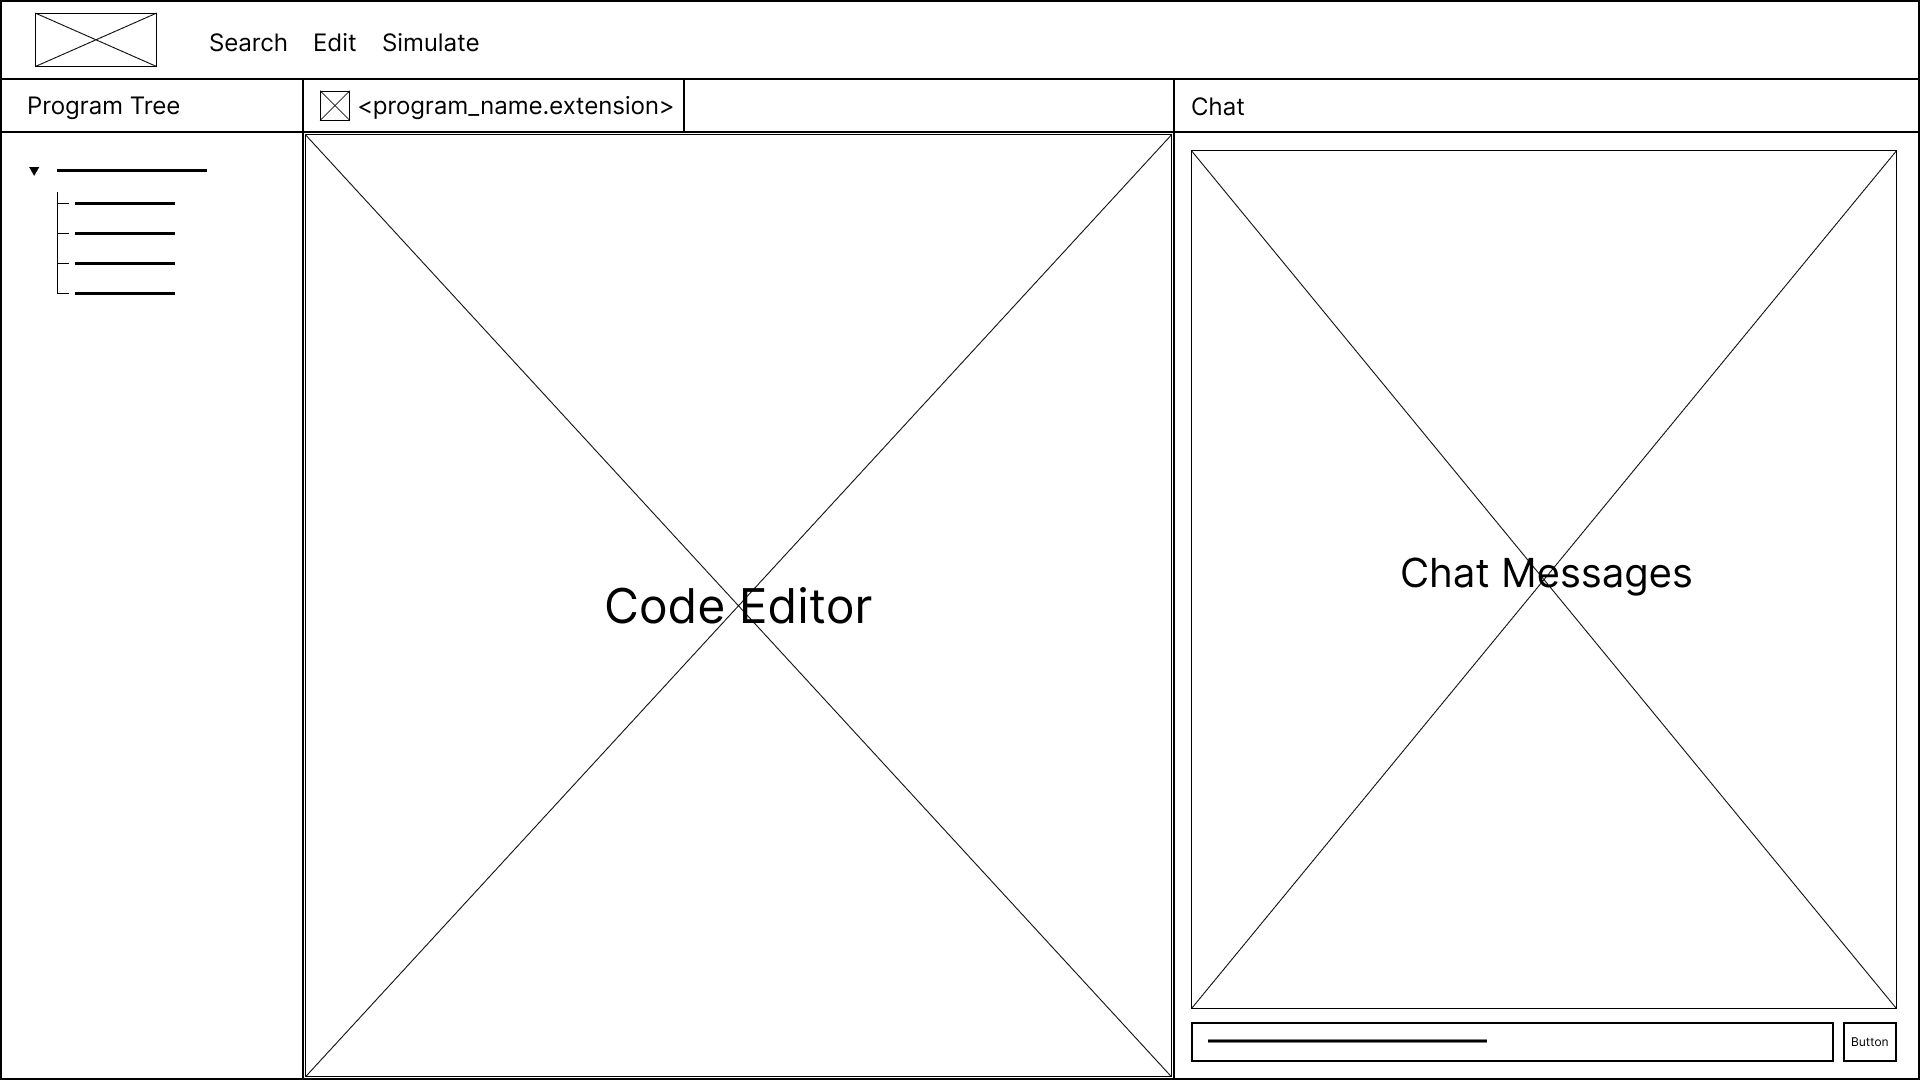
\includegraphics[width=\columnwidth]{media/lofi-edit-tab.png}
    \caption{{Low-fidelity wireframe of the edit interface.}}
    \label{fig:design:lofi_edit}
\end{figure}

The frontend should also preserve interaction state across workspaces. When a user transitions from the search workspace to the editor workspace, the selected program, search context, and assistant context should remain available. The client application should therefore maintain shared application state for the active program, program modifications, and conversational context throughout the interaction workflow.


\section{Client-Server Interaction}
The frontend should communicate with the backend through a REST-based API. A REST architecture provides a clear separation between user-interface concerns and backend functionality such as retrieval, artifact management, and language-model orchestration. This separation improves modularity and allows frontend and backend components to evolve independently through well-defined interfaces.

A REST-based design is also well suited to the interaction patterns of the system. Operations such as searching for robotic programs, retrieving artifacts, and submitting assistant requests naturally follow a request-response structure, making REST an appropriate and lightweight integration approach.

Using standard HTTP-based communication additionally simplifies interoperability with external systems and future extensions of the platform. It also allows the frontend to remain independent of backend implementation details, which supports maintainability and flexibility as the assistant architecture evolves.

Figure \ref{fig:design:search_sequence} shows the communication pattern for program discovery using semantic search. The client should submit a natural-language query through \texttt{POST /api/search}, after which the REST API should obtain a query embedding and use it to search the \texttt{program\_metadata} collection in the vector database. This is an important design distinction: the search interaction should operate over metadata-oriented vector representations, not over the full program code. The response should therefore contain ranked, discovery-oriented results together with the associated \texttt{program\_id}, rather than complete program artifacts. A design in which the full program is attached as metadata for each embedding was considered, but rejected because it would increase payload size, reduce responsiveness during result exploration, and weaken the separation between semantic retrieval and artifact access. Search failure should likewise remain explicit at the API boundary, so the client can present a clear error state to the user.

\begin{figure}[H]
    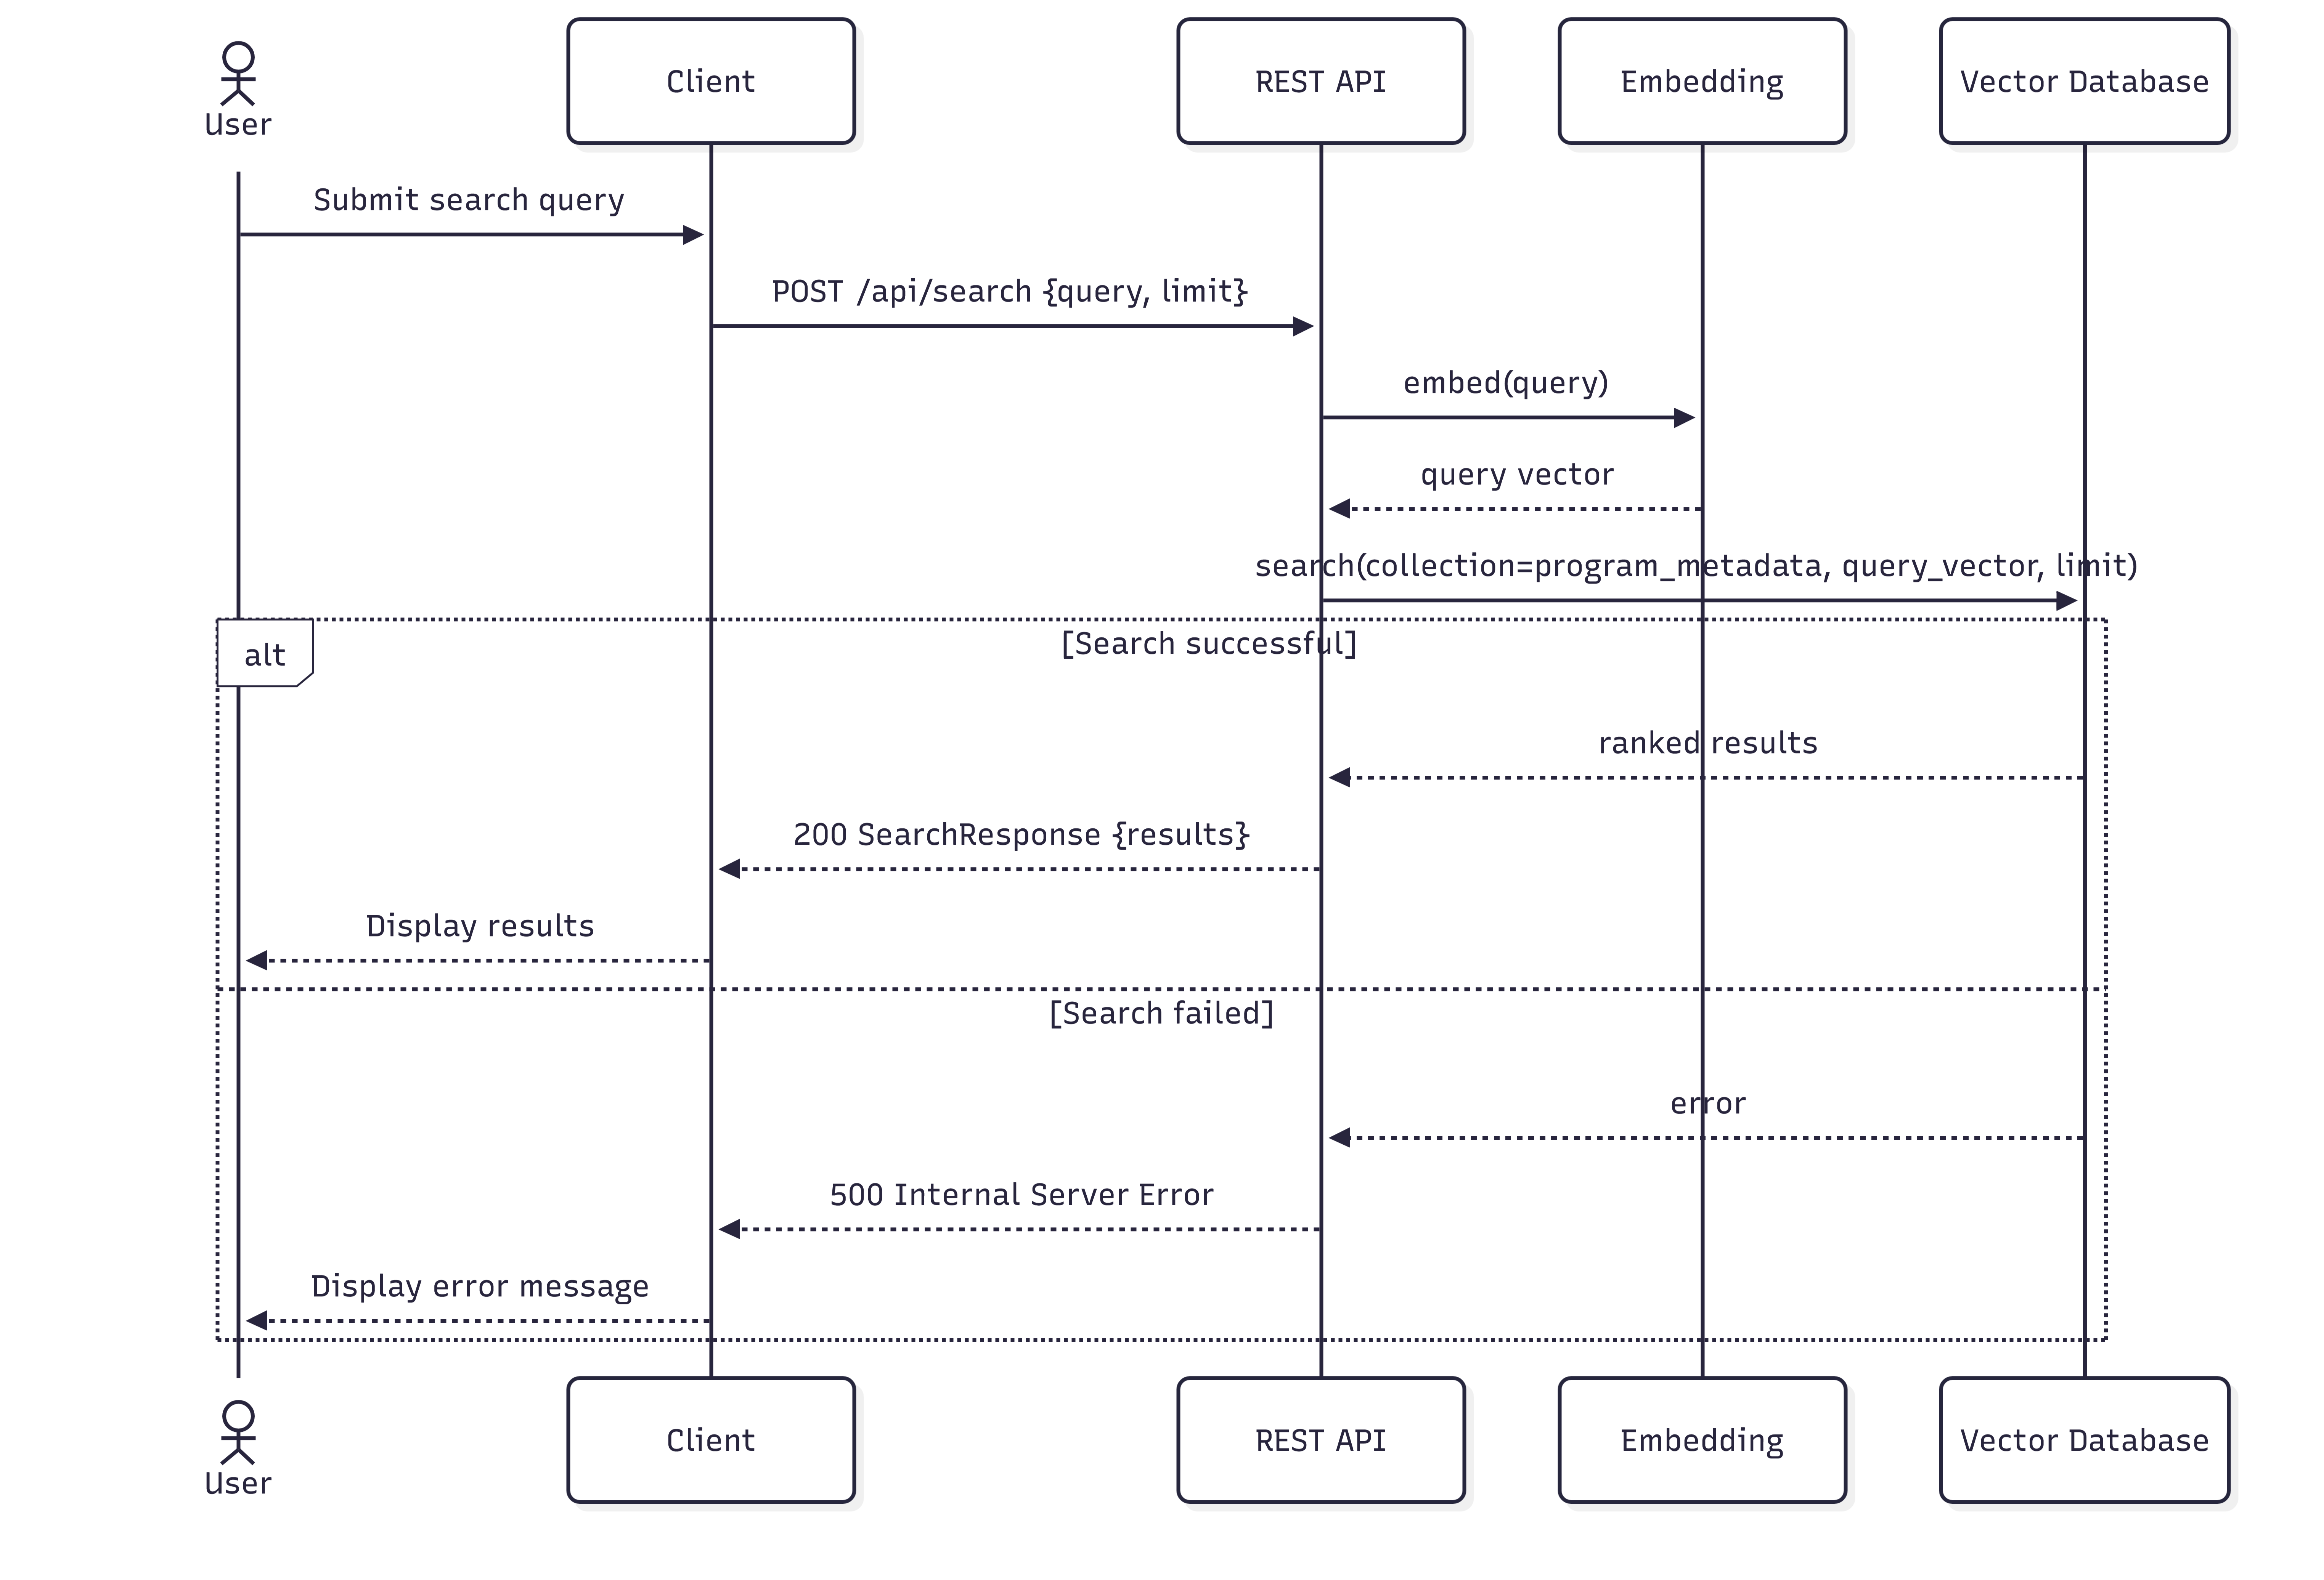
\includegraphics[width=\columnwidth]{media/search-sequence-diagram.png}
    \caption{{Sequence diagram illustrating the communication flow for the search functionality in the robot program editor.}}
    \label{fig:design:search_sequence}
\end{figure}

Once the user selects a program, the frontend should transition to the editor workspace and request the complete artifact through \verb|GET /api/programs/{program_id}/json|, as illustrated in Figure \ref{fig:design:loadProgram_sequence}. The API should resolve this request by calling \texttt{get\_program(program\_id)} on the ProgramStore and returning the corresponding \texttt{program\_json} when the program is found, or a not-found response otherwise. This two-stage interaction reflects a deliberate architectural separation between retrieval and artifact access. The ProgramStore should be a minimal artifact store keyed by \texttt{program\_id}, with the full program representation \texttt{program\_json} held separately from the vector collection. The same \texttt{program\_id} should therefore also be preserved as linking metadata in the search results, allowing a program discovered through semantic search over metadata to be resolved to the stored program artifact used by the editor.

\begin{figure}[H]
    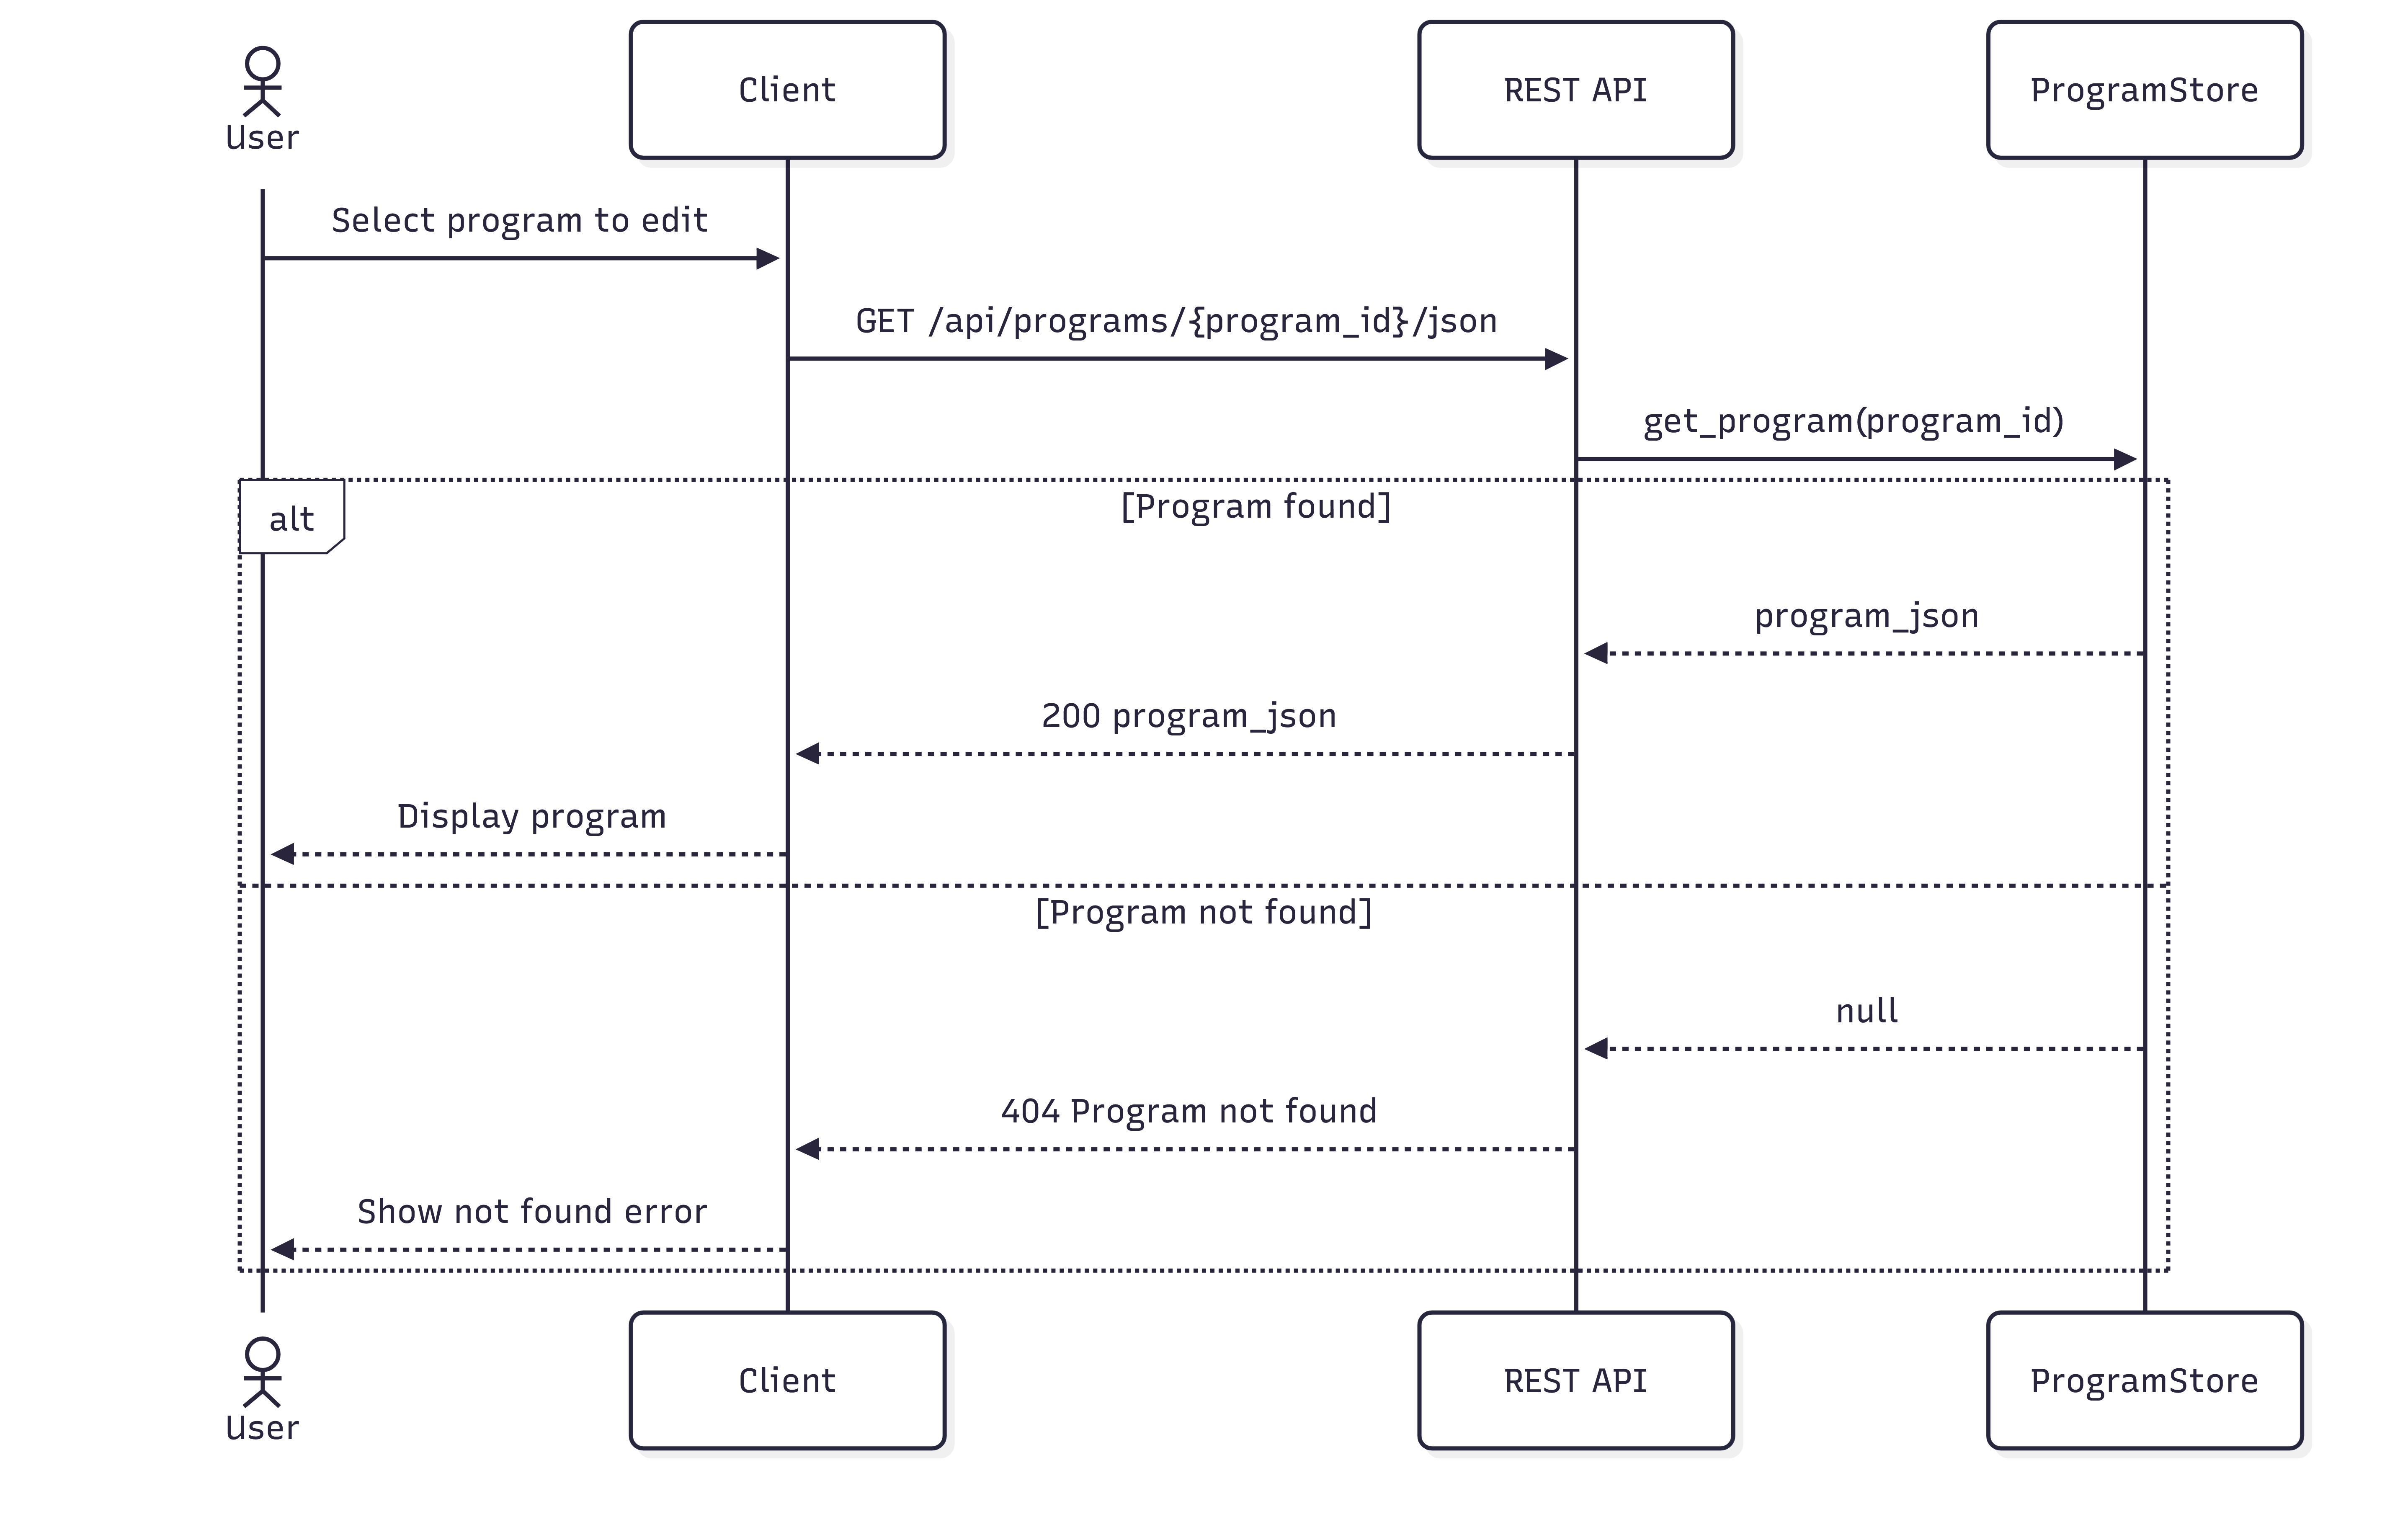
\includegraphics[width=\columnwidth]{media/loadProgram-sequence-diagram.png}
    \caption{{Sequence diagram illustrating the communication flow for the load program functionality in the robot program editor.}}
    \label{fig:design:loadProgram_sequence}
\end{figure}

% \begin{figure}[H]
%     \centering
%     \includegraphics[width=0.3\columnwidth]{media/programStore-table.png}
%     \caption{{ProgramStore schema.}}
%     \label{fig:design:programStore_table}
% \end{figure}

Figure \ref{fig:design:chat_sequence} illustrates the assistant interaction within the editor workspace. The client should submit chat requests through \texttt{POST /api/chat} together with the user message and optional program context derived from the currently loaded artifact. The orchestrator is responsible for agentic assistant functionality, including the loop of up to \texttt{max\_steps}. In each step, the tool-enabled agent should use the language model to decide whether retrieval is needed, use the embedding component and vector database when relevant tool calls are required, and then generate a final response from the gathered context.

\begin{figure}[H]
    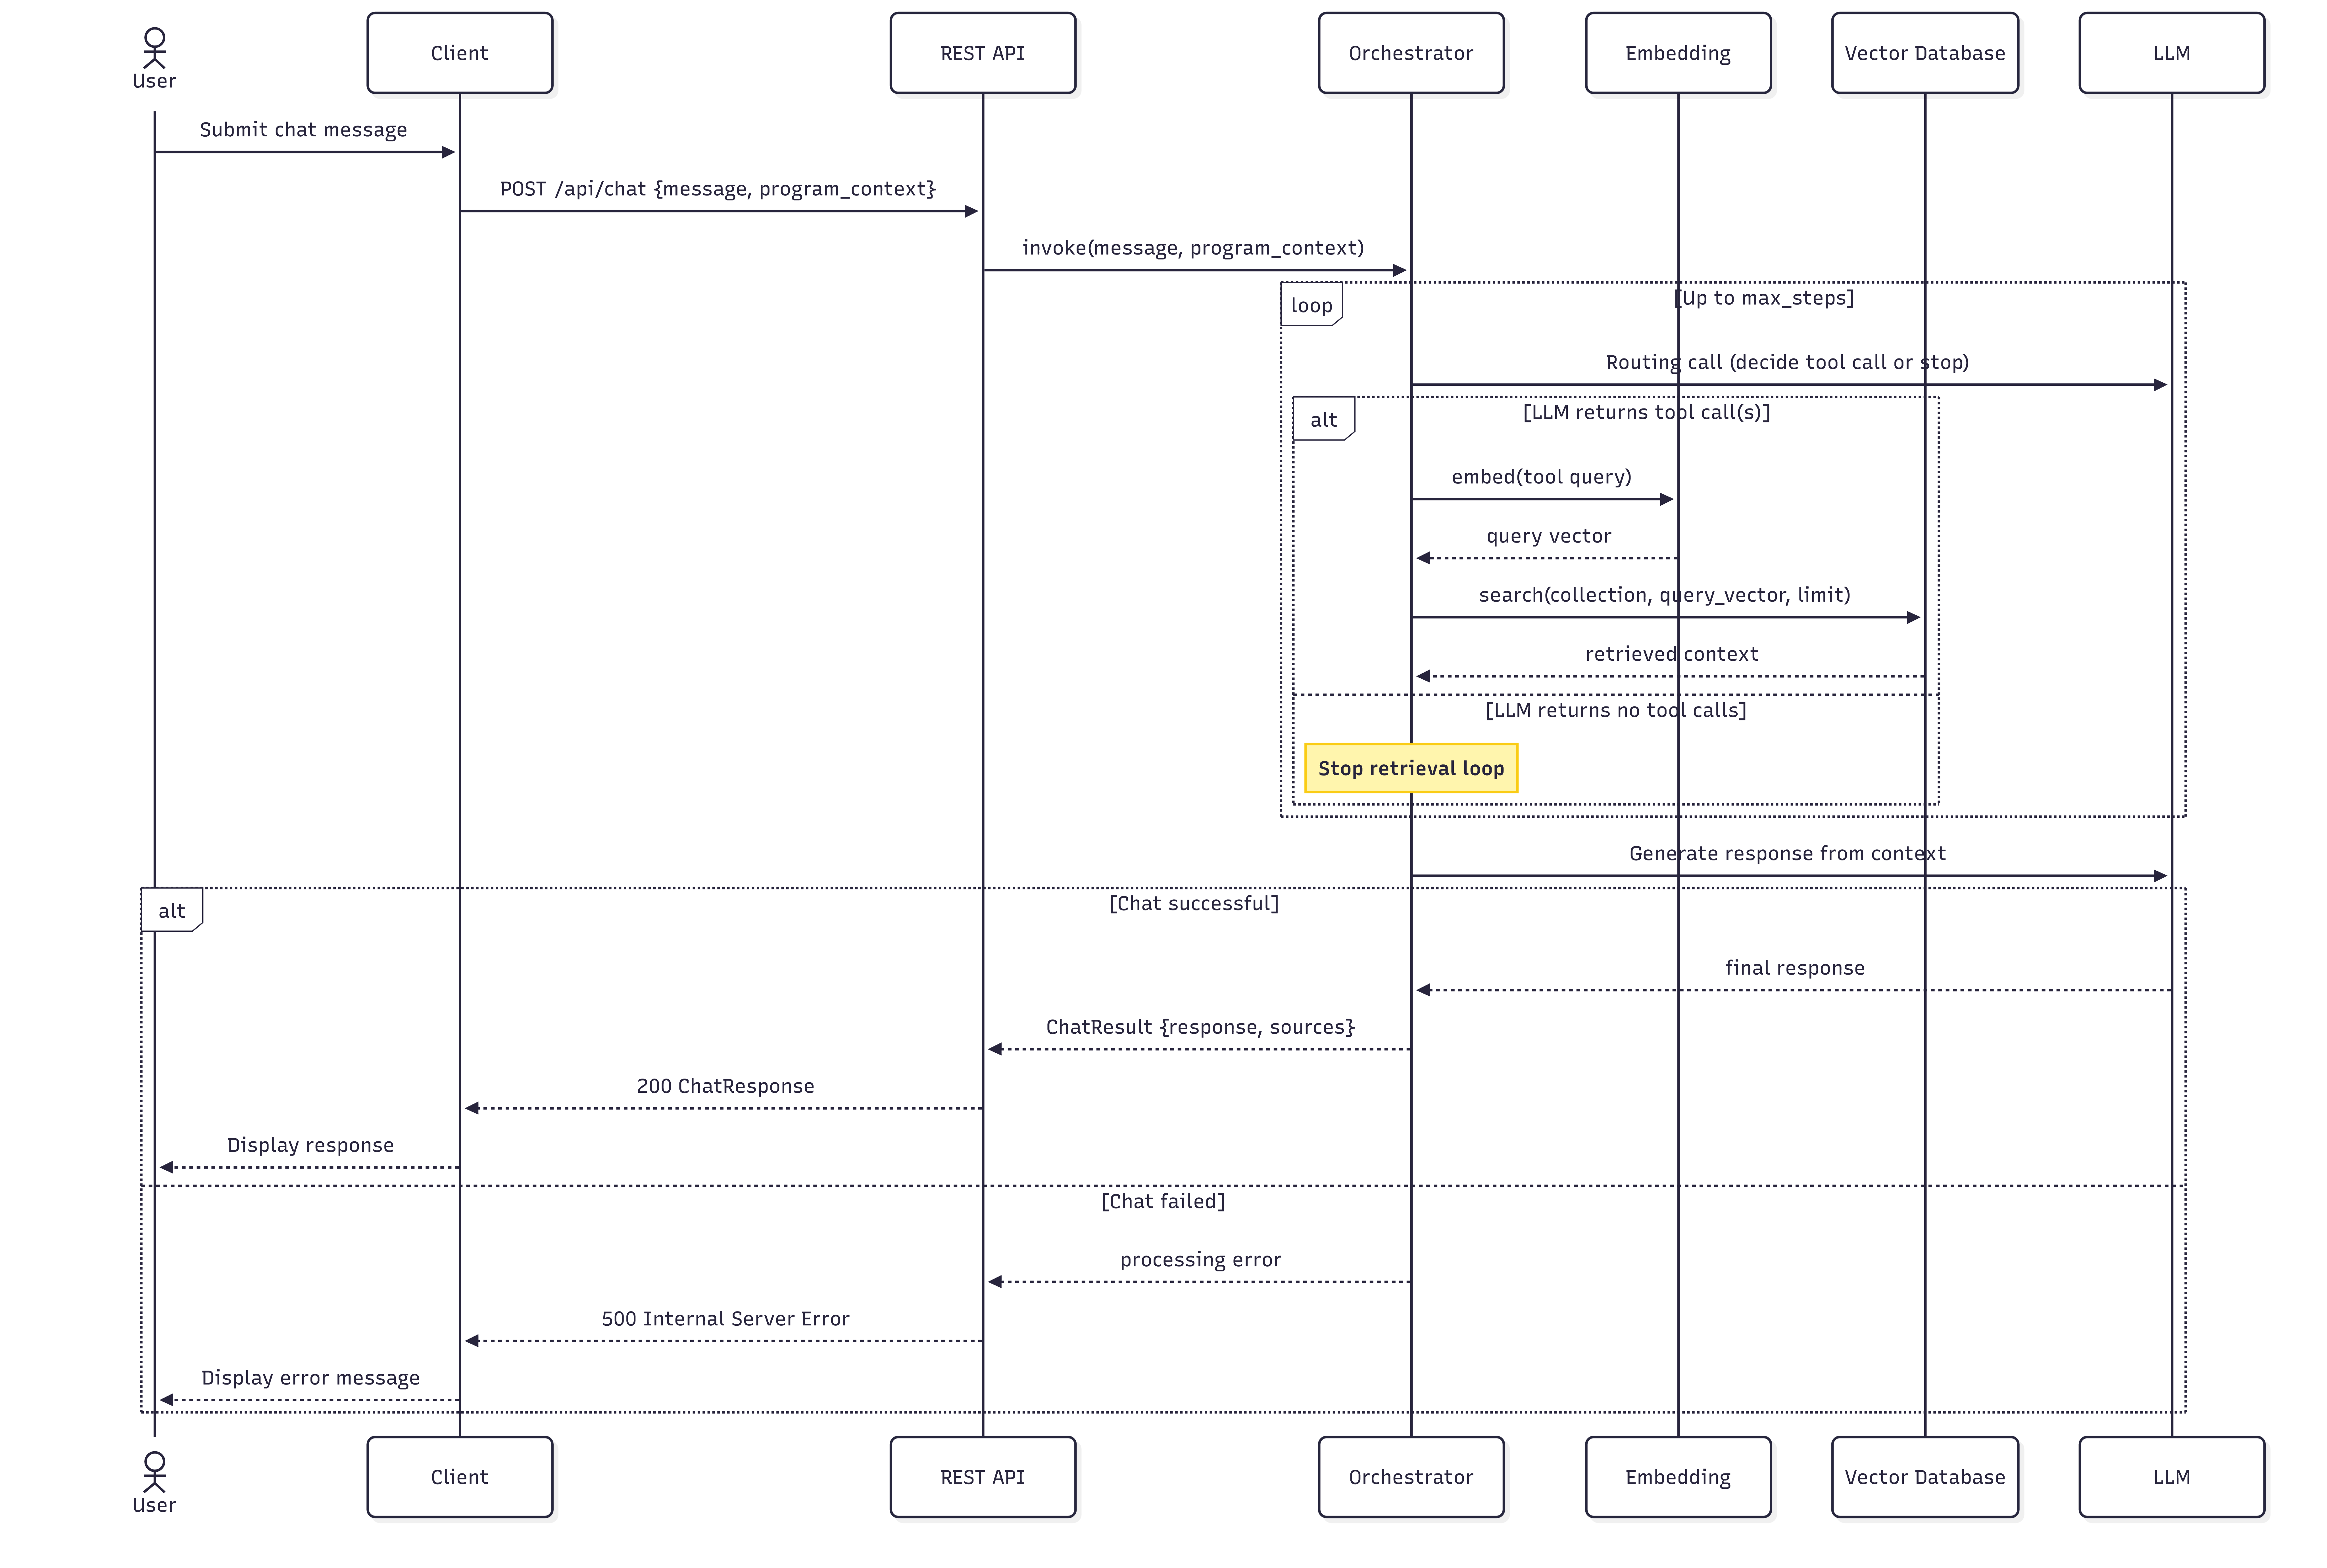
\includegraphics[width=\columnwidth]{media/chat-sequence-diagram.png}
    \caption{{Sequence diagram illustrating the communication flow for the chat functionality in the robot program editor.}}
    \label{fig:design:chat_sequence}
\end{figure}


\section{Technologies}
This section discusses the primary technology choices made for the system implementation and the considerations that motivated these selections.

\subsection{Backend}
The backend is responsible for retrieval orchestration, language-model interaction, data management, and communication with the frontend. The implementation should support rapid development, strong ecosystem support for AI tooling, and integration with modern machine-learning infrastructure.

Python was selected as the backend programming language. Python is widely adopted within the AI and machine-learning community and provides mature libraries and frameworks for AI development. This significantly reduces implementation complexity and improves compatibility with emerging AI infrastructure. While languages such as Java, C++, or Go may provide stronger performance characteristics, Python offers a more suitable balance between development efficiency, ecosystem maturity, and rapid research-oriented experimentation for the scope of this project.

\subsubsection{AI Infrastructure and Orchestration}
The assistant orchestration layer should support tool invocation, retrieval workflows, prompt management, and integration with language models. Several orchestration frameworks exist for LLM-based systems, including LangChain, LlamaIndex, and custom orchestration pipelines.

The project adopts LangChain, as the orchestration framework. LangChain provides abstractions for tool-based reasoning, retrieval workflows, prompt composition, and conversational interaction, which align well with the ReAct-inspired assistant architecture adopted in the project. LangChain simplifies integration between language models, retrieval pipelines, and external tools while remaining sufficiently flexible for experimentation with orchestration logic.

Alternative approaches based on fully custom orchestration pipelines would provide greater architectural control and potentially lower abstraction overhead. However, they would also require substantially more implementation effort for functionality already provided by existing frameworks.

For language-model serving, the system adopts Ollama. Ollama provides a lightweight local inference environment for running language models through a standardized interface. This simplifies experimentation with different models. Running models locally reduces dependence on external cloud services and avoids expensive API usage. Cloud-hosted APIs remain a relevant alternative, particularly for accessing larger models, but local model hosting is sufficient for development and experimentation.

\subsubsection{Storage}
The system requires storage for both semantic retrieval and structured artifact management. These requirements are handled through separate storage technologies optimized for their respective workloads.

For semantic retrieval, the project adopts Qdrant as the vector database. Vector databases are specifically designed for efficient similarity search in high-dimensional embedding spaces and therefore align naturally with the retrieval requirements of retrieval-augmented generation systems. Qdrant provides efficient vector indexing, metadata filtering, and good integration with Python-based AI tooling. Alternative vector databases such as ChromaDB, Pinecone, or Weaviate were also relevant options. However, Qdrant offers a lightweight self-hosted deployment model together with strong retrieval performance and mature ecosystem support.

Structured program artifacts and metadata should be stored separately from vector embeddings. For this purpose, the project adopts SQLite as the primary artifact store. SQLite provides a lightweight relational database with minimal deployment complexity while still supporting structured queries, indexing, and transactional consistency. For the scale and scope of this project, SQLite provides sufficient performance without introducing the operational overhead associated with larger database systems such as PostgreSQL or MySQL.

\subsubsection{Communication}
Communication between frontend and backend components should be exposed through a REST-based API. The backend API framework should therefore support asynchronous request handling, structured data validation, and integration with the Python-based backend infrastructure.

The project adopts FastAPI as the backend API framework. FastAPI provides a lightweight and modern framework for building REST APIs in Python with support for asynchronous operations and automatic request validation. These features simplify implementation of conversational AI endpoints and retrieval-oriented APIs while integrating naturally with the existing backend.

Alternative frameworks such as Flask or Django were also considered. Flask provides a simpler and highly flexible framework, while Django offers a more comprehensive full-stack architecture. However, FastAPI provides a good balance between lightweight design and modern API-oriented development for the needs of this project.


\subsection{Frontend}
The frontend should support interactive assistant workflows, program inspection, and workspace navigation while remaining responsive and extensible. The implementation therefore benefits from technologies that support component-based user interfaces and dynamic client-side interaction.

The project adopts React as the frontend framework. React provides a component-based architecture that aligns well with the modular structure of the interface, including separate search, editor, and assistant views. Its reactive rendering model is also well suited for AI-assisted interaction such as conversational interfaces.

Alternative frontend frameworks such as Angular or Vue were also relevant options. Angular provides a more opinionated full-framework architecture, while Vue offers a lightweight and approachable component model. However, React was selected due to its broad ecosystem support, flexibility, and widespread adoption within modern web application development.

The frontend additionally adopts React Router for client-side navigation between application workspaces. Since the interface separates search-oriented workflows from program comprehension and modification workflows, client-side routing provides a structured way to manage navigation and preserve interaction state across views without requiring full page reloads. This supports a smoother and more application-like user experience during iterative development tasks.

For program editing and inspection, the frontend adopts the Monaco Editor, which provides the editor infrastructure used in Visual Studio Code. Monaco offers features such as syntax highlighting, structured code editing, and extensibility for future language-support capabilities. This makes it well suited for robotic program inspection and modification tasks, where readability and structured interaction with program artifacts are important.

\chapter{Implementation} \label{sec:implementation}
This chapter describes the implemented prototype following the architecture outlined in the above chapter (see Chapter~\ref{chapter:design}).

\section{Data Pipeline}
The knowledge base is prepared by an ingestion script \texttt{data\_pipeline/build.py}. On each run, the script loads configuration, initializes the embedding model, vector database, program store, program loader, and document loader, then builds the retrieval indexes from the robot programs and documentation data.

Keeping this workflow offline avoids performing data transformation, chunking, and embedding generation at query time. At the time of writing, the corpus consists of 8 robot programs with corresponding metadata files and 22 PDF documents, producing 8 metadata program descriptions, 126 program code chunks, and 2612 documentation chunks.

\subsection{Program Processing}
Robot programs (\texttt{.urpx} files) are loaded together with the associated \texttt{meta.json} files. Program ingestion produces two text representations: one based on the metadata and one based on the program code.

The first representation is a metadata summary. The outer loading loop iterates over all program directories, opens each \texttt{meta.json} file, and calls a helper that synthesizes exactly one \texttt{ProgramChunk} for that program (see Code~\ref{listing:implementation:program_metadata_loop}).

\begin{listing}[H]
	\begin{minted}[fontsize=\small, breaklines]{python}
programs = []
for program_dir in program_dirs:
    meta_file = program_dir / "meta.json"
    with open(meta_file, "r", encoding="utf-8") as f:
        metadata = json.load(f)

    programs.append(self._synthesize_program(program_dir.name, metadata))
	\end{minted}
	\caption{Load each program's metadata file and create one metadata chunk per program.}
	\label{listing:implementation:program_metadata_loop}
\end{listing}

% \begin{listing}[H]
% 	\begin{minted}[fontsize=\small, breaklines]{python}
% def _synthesize_program(self, program_dir: str, metadata: Dict[str, Any]) -> ProgramChunk:
% 	program_name = metadata.get("name", program_dir)
% 	robot_type = metadata.get("robotType", "Unknown")
% 	application_type = metadata.get("applicationType", "General")
% 	gripper_types = metadata.get("gripperType", [])
% 	object_type = metadata.get("objectType", [])
% 	actions = metadata.get("actions", [])
% 	data_available = metadata.get("dataAvailable", "")
% 	components = metadata.get("components", [])
%
% 	gripper_text = ", ".join(gripper_types) if gripper_types else "not specified"
% 	object_text = ", ".join(object_type) if object_type else "not specified"
% 	action_text = ", ".join(actions) if actions else "not specified"
% 	component_text = " | ".join(components) if components else "not specified"
%
% 	chunk_text = (
% 		f"Program: {program_name}. "
% 		f"Robot type: {robot_type}. "
% 		f"Application: {application_type}. "
% 		f"Gripper: {gripper_text}. "
% 		f"Object type: {object_text}. "
% 		f"Actions: {action_text}. "
% 		f"Components: {component_text}. "
% 		f"Data available: {data_available}."
% 	)
%
% 	return ProgramChunk(
% 		program_id=program_dir,
% 		program_name=program_name,
% 		chunk_text=chunk_text,
% 		metadata=metadata,
% 	)
% 	\end{minted}
% 	\caption{Helper used to synthesize the metadata summary text stored in each \texttt{ProgramChunk}.}
% 	\label{listing:implementation:program_metadata_chunk}
% \end{listing}

After the metadata file is loaded, \texttt{\_synthesize\_program(...)} extracts the program name, robot type, application type, gripper type, object type, actions, components, and data-availability field. Missing values are filled with defaults. List-valued attributes are converted into readable strings before the helper concatenates them into one natural-language sentence stored as the \texttt{chunk\_text} of the resulting \texttt{ProgramChunk} datatype. The original metadata is retained alongside it for later reference. This approach allows retrieval to operate on a natural-language summary while still preserving access to the structured metadata when needed.

Code~\ref{listing:implementation:program_metadata_example} shows an example of that synthesized text for one of the indexed programs.

\begin{listing}[H]
	\begin{minted}[fontsize=\small, breaklines]{text}
Program: Program2. Robot type: UR5. Application: Pick and Place. Gripper: 2FG7. Object type: Cube. Actions: moveJ, moveJ, release, moveL, grip, moveL, moveJ, moveL, release, moveL, moveJ. Components: UR5 | Gripper 2FG7. Data available: Robot Operational Data | Event Data.
	\end{minted}
	\caption{Example of a metadata chunk.}
	\label{listing:implementation:program_metadata_example}
\end{listing}

The second representation targets code-level retrieval and may produce multiple chunks per program. Each \texttt{.urpx} file is converted to JSON and traversed recursively by \texttt{\_collect\_nodes(...)} to locate program behavior nodes (actions). For each node, \texttt{\_extract\_action\_name(...)} tries to extract an action from parameters such as \texttt{moveType} or \texttt{action}. When an action is available, a program code chunk of type \texttt{ProgramCodeChunk} containing a natural-language summary (\texttt{chunk\_text}) and the JSON code snippet (\texttt{snippet\_text}) is created. Additional fields such as identifiers, line numbers, metadata, and chunk index are also attached to each chunk for later reference.

Code~\ref{listing:implementation:program_code_chunk} shows the code-level chunk construction.

\begin{listing}[H]
	\begin{minted}[fontsize=\small, breaklines]{python}
node_entries = []
self._collect_nodes(
	node=data.get("program", {}).get("programContent", {}),
	path="program.programContent",
	output=node_entries,
)

action_entries = []
for entry in node_entries:
	action_name = self._extract_action_name(entry)
	if action_name:
		entry["action_name"] = action_name
		action_entries.append(entry)

chunks = []
for idx, entry in enumerate(action_entries):
	chunks.append(
		ProgramCodeChunk(
			# program_id, program_name, start_line/end_line,
			# section_name, and metadata are also stored
			chunk_text=self._build_action_summary(
				program_name, entry, action_entries, idx
			),
			snippet_text=self._build_readable_snippet(entry),
		)
	)
	\end{minted}
	\caption{Program code chunk construction.}
	\label{listing:implementation:program_code_chunk}
\end{listing}

Code~\ref{listing:implementation:program_code_chunk_example} shows an example of the natural-language summary for one of the action nodes in the indexed programs.

\begin{listing}[H]
	\begin{minted}[fontsize=\small, breaklines]{text}
Program Program5 action snippet. Action: moveL; Node type: ur-move-to; Label: Point_3 | 30 % | 9 %; moveType: moveL; variable: Point_3; Previous actions: release; Next actions: moveJ.
	\end{minted}
	\caption{Example of a code-level chunk summary.}
	\label{listing:implementation:program_code_chunk_example}
\end{listing}

\subsection{Documentation Processing}
Technical documentation is processed with a dedicated PDF loader built on PyMuPDF. The extracted text is cleaned before chunking to remove common PDF artifacts such as line-break hyphenation and irregular whitespace. The cleaned text is then segmented section by section with a sentence-aware sliding window using a chunk size of 300 tokens and an overlap of 48 tokens.

Within each section, the loader first fills a chunk with as many complete sentences as fit within the target window. It then steps backward by the configured overlap so that neighboring chunks share some context. Very small trailing chunks are merged into adjacent chunks to reduce underspecified retrieval results near boundaries. Each final documentation chunk retains its document name, page number, and chunk index, yielding 2612 searchable chunks across the current document corpus.

The default chunk size of 300 tokens was chosen as a balance between contextual completeness and retrieval specificity. Smaller chunks more often separated short procedure descriptions, warnings, and parameter explanations that were semantically related, while much larger chunks increased the amount of irrelevant surrounding text returned with each hit. The overlap of 48 tokens was chosen to preserve continuity across chunk boundaries without introducing excessive duplication. In practice, this overlap was large enough to carry short transitions and neighboring procedural context into the next chunk, but small enough to avoid filling the index with near-duplicate passages.

The implementation does not compute exact token counts with the embedding model tokenizer. Instead, it uses a lightweight approximation of roughly four characters per token when translating the configured token budget into chunk-size and overlap limits. The main advantage is simplicity and performance: the chunker remains fast and independent of a model-specific tokenizer, which was useful during repeated local indexing runs. The disadvantage is reduced precision, since actual token counts vary with formatting, symbols, and vocabulary. As a result, some chunks will be somewhat shorter or longer than the target. This is also relevant with respect to the embedding model itself, because an embedding backend has a finite input window. The current implementation does not enforce a hard model-specific maximum token count, so the conservative 300 tokens with 48 token overlap also serves as a safety margin against input-limit issues, although the embedding models used have a large enough window that this was not a problem.

\subsection{Embedding and Indexing}
Embedding is handled through an \texttt{EmbeddingModel} abstraction. The wrapper reads the model name, base URL, request timeout, batch size, and embedding dimension from the data-pipeline configuration file and uses Ollama through \texttt{OllamaEmbeddings}. Its \texttt{embed()} method accepts either one string or a list of strings. For batch inputs, it slices the texts into batches of 64, calls the embedding backend for each batch, and returns a NumPy array with one vector per text. For a single query string, it returns one vector of length \texttt{embedding\_dimension}. The Qdrant vector database reads the same \texttt{embedding\_dimension} setting from config, so the embedding layer and the vector database share a single source of truth.

During early development, a smaller embedding model was used because it supported faster local indexing runs and quicker iteration on the retrieval pipeline. In the final configuration, this was replaced with \texttt{qwen3-embedding:8b}. The larger model increased indexing time, but it also improved retrieval quality.

Ingestion is implemented in \texttt{data\_pipeline/build.py}. The script initializes the embedding model, vector store, program store, and loaders, loads the three corpora, and then ingests each corpus into separate collections. For each corpus, it extracts the \texttt{chunk\_text} field, calls \texttt{embed()}, creates the Qdrant collection, and upserts one point per chunk. In Qdrant, a point is one stored vector record consisting of an id, the embedding vector, and a payload dictionary with metadata fields. The three collections are \texttt{robot\_programs} for metadata, \texttt{robot\_program\_code} for code snippets, and \texttt{documentation} for documentation.

To search a collection, the \texttt{VectorStore.search(collection\_name, query\_embedding, limit)} method is exposed. The method accepts the collection name, the query embedding vector, and the number of results to return. It then calls \texttt{query\_points(...)} on the Qdrant client, which performs a cosine similarity search and returns the top hits with their payloads and scores.


\section{Backend}
The backend is implemented as a FastAPI application with an orchestration layer. At startup, the service constructs an \texttt{Orchestrator} instance. The \texttt{Orchestrator} owns the embedding model interface, vector store connection, language model client, retrieval tools, and conversation memory.

It exposes an \texttt{invoke(...)} method that accepts a user query and optional program context. The method performs the agentic orchestration loop and then synthesizes a final response based the user query, tool-use, conversation history, and program context.

In the current implementation, both the agentic orchestration loop and the final response synthesis use the same language model, \texttt{qwen3.5:2b}.

\subsection{Agentic Loop}
The agentic functionality of the orchestrator is implemented in the \texttt{\_agentic\_loop(...)} method. Using the LangChain tool interface, the orchestrator defines three retrieval tools that the agent can call to search the program-metadata, program-code, and documentation collections. The agent is prompted to decide which tools to call and when to stop retrieving, allowing it to adaptively gather information based on the user query and the results obtained so far.

The retrieval process is implemented as an agentic loop with a fixed maximum of five steps. For each user query, the helper \texttt{\_assemble\_agent\_messages(...)} assembles the initial message list by combining the system prompt, the current query, optional program context, and conversation history. This list consists of LangChain message objects. In the current implementation, the initial entries are a \texttt{SystemMessage} containing the system prompt and \texttt{HumanMessage} objects containing the user query and additional user provided context. During the loop, the agent's reply message is appended to the same list, and each executed retrieval tool appends a \texttt{ToolMessage} containing the returned JSON payload. The agent can then stop immediately or invoke one or more retrieval tools, depending on whether the query can be answered from the current message state. After each tool call, the returned tool result is appended to the same message state and the model decides whether additional retrieval is still necessary. The five-step limit prevents the retrieval phase from continuing indefinitely in case no relevant results are returned from the tool calls.

Code~\ref{listing:implementation:agentic_loop} shows the agentic loop. The key detail is that the agent repeatedly receives the updated message state, including prior tool outputs, and can therefore stop as soon as sufficient evidence has been gathered.

\begin{listing}[H]
	\begin{minted}[fontsize=\small, breaklines]{python}
	messages = self._assemble_agent_messages(...)
	max_steps = 5

	for step_num in range(1, max_steps + 1):
		response = self.agent_llm.invoke(messages)
		messages.append(response)

		tool_calls = getattr(response, "tool_calls", []) or []
		if not tool_calls:
			sources = collect_sources_from_tool_messages(messages)
			return sources, False

		for tool_call in tool_calls:
			messages.append(self._dispatch_tool_call(tool_call, step_num, ...))

	sources = collect_sources_from_tool_messages(messages)
	return sources, True
	\end{minted}
	\caption{Agentic orchestration loop.}
	\label{listing:implementation:agentic_loop}
\end{listing}

When the agent model decides to stop (no tools called), \texttt{collect\_sources\_from\_tool\_messages(...)} filters the accumulated LangChain message list for \texttt{ToolMessage} entries produced by earlier tool calls, parses their JSON payloads, and collects the retrieved documents into one shared source list. This list is used for response synthesis regardless of which tools were called, so that the synthesis stage can reason over all retrieved information without needing to know which tool produced which result. If the loop reaches the five-step limit, the same collection process is applied to gather whatever sources were retrieved up to that point, but a boolean flag is set to indicate that retrieval may be incomplete. This allows the synthesis stage to adjust its reasoning and response generation based on whether the retrieval phase was potentially cut short by the step limit.

Code~\ref{listing:implementation:tool_registration} shows the helper that defines tools. Three retrieval tools are implemented. Each tool uses the \texttt{VectorStore.search(...)} method that performs a search over one of the three vector collections. The tools are given descriptive names such as \texttt{search\_robot\_programs}, \texttt{search\_robot\_code}, and \texttt{search\_doc\-umentation} to make their purpose clear in the system prompt. The final return statement returns the three tool objects as a list. The orchestrator later binds the list of tools to the agent model with \texttt{base\_llm.bind\_tools(...)} in the \texttt{\_bind\_agent\_llm(...)} method.

\begin{listing}[H]
	\begin{minted}[fontsize=\small, breaklines]{python}
def _define_tools(self):
	@tool("search_robot_programs")
	def search_robot_programs(query, limit=3):
		return self._search_collection(self.programs_collection, query, limit)

	@tool("search_robot_code")
	def search_robot_code(query, limit=3):
		return self._search_collection(self.program_code_collection, query, limit)

	@tool("search_documentation")
	def search_documentation(query, limit=3):
		return self._search_collection(self.documentation_collection, query, limit)

	return [search_robot_programs, search_robot_code, search_documentation]
	\end{minted}
	\caption{Tool definitions.}
	\label{listing:implementation:tool_registration}
\end{listing}

\subsubsection{Agent Prompt}
The agent behavior is shaped not only by the loop structure, but also by the system prompt produced by \texttt{get\_agentic\_system\_prompt()} in \texttt{backend/llm/prompts.py}. This prompt is inserted as the first \texttt{System\-Message} in the agent message list and frames the model as a retrieval controller rather than as the final answer generator. That separation of roles is important: during the retrieval stage, the model is instructed to gather evidence and decide whether to continue retrieving, while response synthesis is handled later by a separate prompt. The full prompt is shown in Code~\ref{listing:appendix:agent_prompt} in Appendix~\ref{appendix:implementation-prompts}.

The agent system prompt combines several prompt-engineering techniques. First, it uses \textit{role prompting} by assigning the model the role of an intelligent retrieval assistant for robot programs and documentation. Second, it uses \textit{clear and specific instructions}: the prompt states the model's job explicitly, lists the available tools, and defines a concrete retrieve-evaluate-decide workflow. Third, it uses \textit{constraint setting}. The prompt tells the model not to synthesize the final answer, limits the number of documents and tool calls, and instructs it to stop early when sufficient evidence has already been found. These constraints narrow the model's behavior from general dialogue generation to controlled evidence gathering.

The prompt also uses a constrained form of \textit{chain-of-thought prompting}. It does not ask the model to emit a free-form reasoning trace, but it does force a stepwise reasoning pattern: retrieve context, evaluate relevance and sufficiency, identify gaps, and then decide whether to stop or continue. In addition, the prompt uses \textit{few-shot learning} through four concrete decision scenarios. Those examples demonstrate the desired policy for different classes of questions, such as example-program search, technical-configuration questions, program-modification requests, and general-knowledge queries that should bypass retrieval entirely. The prompt further uses \textit{delimiter and structure cues} in the form of section headings, numbered workflow stages, and clearly separated STOP/CONTINUE conditions, which makes the instruction hierarchy easier for the model to follow.

Together, these prompt elements complement the code-level constraints in the orchestrator. The Python code enforces the message flow and the five-step limit, but the prompt shapes the model's actual retrieval strategy: which tool it selects first, whether it broadens the search after weak results, and when it decides that the available evidence is sufficient.


\subsection{Context Management}
Context management keeps the message state small enough that each request still has room for the current query, the system prompts, retrieved documents, optional program context from the editor, and recent conversation history. In this application, that balance matters because both retrieval and synthesis depend on having enough space for robot-program examples and documentation passages from the current turn.

The current implementation combines \textit{system-prompt preservation} with a \textit{sliding window} over recent conversation turns. The agent and synthesis prompts are inserted separately each time the message lists are assembled, so the main instructions stay stable from turn to turn. Conversation history is handled by the \texttt{ConversationMemory} component in \texttt{backend/orchestrator/memory.py}, which stores recent user and assistant messages and makes them available again for later requests. This gives the assistant short-term continuity across follow-up questions while keeping the prompt instructions fixed.

The size of the stored history is controlled by a budget derived from the size of the model context window. Of the available context window, 20\% is reserved for conversation history. This is used as a practical fixed budget for recent dialogue, so that most of the context window remains available for the current query, the system prompts, retrieved sources, and optional program context from the editor, which can be large. Message size is estimated with a simple heuristic based on character count, word count, and a small fixed overhead per message. When the stored history grows beyond that budget, the component first reduces the number of retained messages and then removes the oldest messages until the history fits again. The system keeps the most recent conversation turns and leaves room for the current-turn material that is most important for retrieval and synthesis.


\subsection{Response Synthesis}
After tool-use, the backend enters a separate synthesis stage implemented in \texttt{\_synthesize\_response(...)}. At this point, the agentic loop has already collected a list of source objects, and the synthesis stage converts those sources into one context block for the language model. For each retrieved item, the backend includes the retrieved text and its source label. For code-related results, it also includes the JSON snippet stored in the payload, so the model can use both the short embedding summary and the underlying program structure. If the user has provided program context from the editor, that content is appended as an additional context block. Recent conversation history is included separately, and a retrieval-status message indicates whether retrieval completed normally or whether the five-step limit was reached. The final answer is therefore generated from four main inputs: the user query, the retrieved sources, optional program context, and recent conversation history.

The synthesis prompt is defined in \texttt{get\_synthesis\_prompt\_template()} in \texttt{backend/llm/prompts.py}. The full prompt is shown in Code~\ref{listing:appendix:synthesis_prompt} in Appendix~\ref{appendix:implementation-prompts}. Unlike the agent stage, this prompt is implemented as a chat prompt with two parts: a \texttt{SystemMessage} that defines the stable response policy, and a \texttt{HumanMessage} that inserts the runtime information for the current turn. The system part tells the model to answer the current query first, use the provided context, treat conversation history as secondary context, acknowledge missing information, and respond in Markdown only. The human part provides the retrieval-status text, the current user query, the primary context assembled from retrieved sources and program context, and the secondary context assembled from recent conversation history.

The synthesis prompt uses several prompt-engineering techniques. It applies \textit{role prompting} by framing the model as a helpful assistant for UR robot programming and technical questions. It uses \textit{clear and specific instructions} by stating exactly which input should be prioritized and how the answer should be grounded in the supplied context. It uses \textit{constraint setting} by instructing the model not to append a separate citations section, to acknowledge uncertainty explicitly, and to state when the available evidence is insufficient. It also uses \textit{output-format specification} through explicit Markdown rules for headings, lists, short paragraphs, and a dedicated limitations section when information is missing or uncertain. In addition, the prompt establishes a clear hierarchy between inputs: the current query is the primary signal, retrieved documents and program context are the primary evidence, and conversation history is only secondary context for continuity.

This design separates evidence gathering from answer generation. The retrieval stage is responsible for deciding what information to collect, while the synthesis stage is responsible for turning the collected evidence into a final user-facing response. In practice, this keeps the response model focused on explanation and answer construction rather than on tool choice, and it ensures that program snippets, documentation passages, user-provided editor context, and recent dialogue are all combined in a single structured prompt before generation.


\subsection{REST API}
The REST API is the connection between the browser frontend and the Python backend. A REST API is a set of URL endpoints that a client can call with standard HTTP methods. In this system, \texttt{GET} is used to fetch stored data, while \texttt{POST} is used to send a query or trigger backend work. The API has two main purposes: it gives the frontend access to stored robot-program artifacts, and it gives the frontend a way to send search requests and assistant queries to the orchestration layer.

The service is implemented with FastAPI in \texttt{backend/main.py} and \texttt{backend/api/routes.py}. FastAPI maps each endpoint to a Python function. At startup, the application creates one \texttt{Orchestrator} instance inside FastAPI's lifespan hook and stores it in the application state, so the route handlers can reuse the same backend services. The application also enables a small CORS configuration. CORS is a browser security rule that decides which web pages are allowed to call a backend service. Here it allows the local React frontend, running on \texttt{localhost}, to access the backend during development.

Request and response formats are defined with Pydantic models. Pydantic is a Python library that checks data types and converts incoming JSON into structured Python objects. \texttt{ChatRequest} contains the user message and optional program context from the editor. \texttt{ChatResponse} packages the final answer together with the returned sources, routing metadata, and a session identifier. The search route uses its own \texttt{SearchRequest} and \texttt{SearchResponse} models.

The API supports the main frontend workflow with a small set of endpoints. \texttt{POST /api/search} is used by the search page. It embeds the query, searches the \texttt{robot\_programs} vector collection, and returns ranked matches with metadata. \verb|GET /api/programs/{program_id}/json| loads the selected program in JSON form for the editor, and \verb|GET /api/programs/{program_id}/download| returns the \texttt{.urpx} file for export. In the current frontend, assistant interaction uses \texttt{POST /api/chat/stream}. The first version of the assistant endpoint was the synchronous \texttt{POST /api/chat} route, which returns one complete JSON response after all retrieval and synthesis steps have finished. Because this interaction is slow, the later \texttt{POST /api/chat/stream} route extends the same orchestration flow with progress updates. It calls \texttt{orchestrator.invoke(...)} in a background thread, stores progress messages in a queue, and sends them back to the browser as Server-Sent Events. Server-Sent Events are a simple one-way streaming format in which the server pushes messages over one open HTTP connection. The chat panel uses these streamed events to show what the assistant is working on before the final response arrives. The editor resets server-side conversation history through \texttt{POST /api/chat/clear-memory}.


\newpage
\section{Frontend}
The frontend is implemented as a single-page React application in \texttt{app/frontend}. It provides the browser interface for program search, program inspection and editing, and assistant interaction. Client-side routing is defined with \texttt{react-router} in \texttt{App.jsx}, which exposes three routes: \texttt{/} for search, \texttt{/edit} for the editor and chat interface, and \texttt{/simulate} as a placeholder for future simulation functionality.

Persistent frontend state is managed with two React context providers. \texttt{EditorContext} stores the selected program identifier, the loaded program payload, the current editor contents, the selected code range, pending program-context snippets, chat history, and the most recent search state. \texttt{ThemeContext} stores the light/dark preference and persists it in \texttt{localStorage}. This allows the loaded program, search state, and assistant conversation to remain available when the user moves between the pages.

The search page (see Figure~\ref{fig:implementation:search_tab}) is implemented in \texttt{ProgramSearch.jsx}. The page focuses on search query input, ranking, and program selection. The interface has gone through multiple iterations of result presentation. An earlier version displayed the raw semantic similarity score for each hit, but these values were interpreted as absolute quality indicators and caused confusion. In the current version, ranking is still based on the semantic score internally, while the UI emphasizes relative order and program metadata labels (robot type, application, gripper, object type, components, and action count) instead of exposing raw scores.

\begin{figure}[H]
	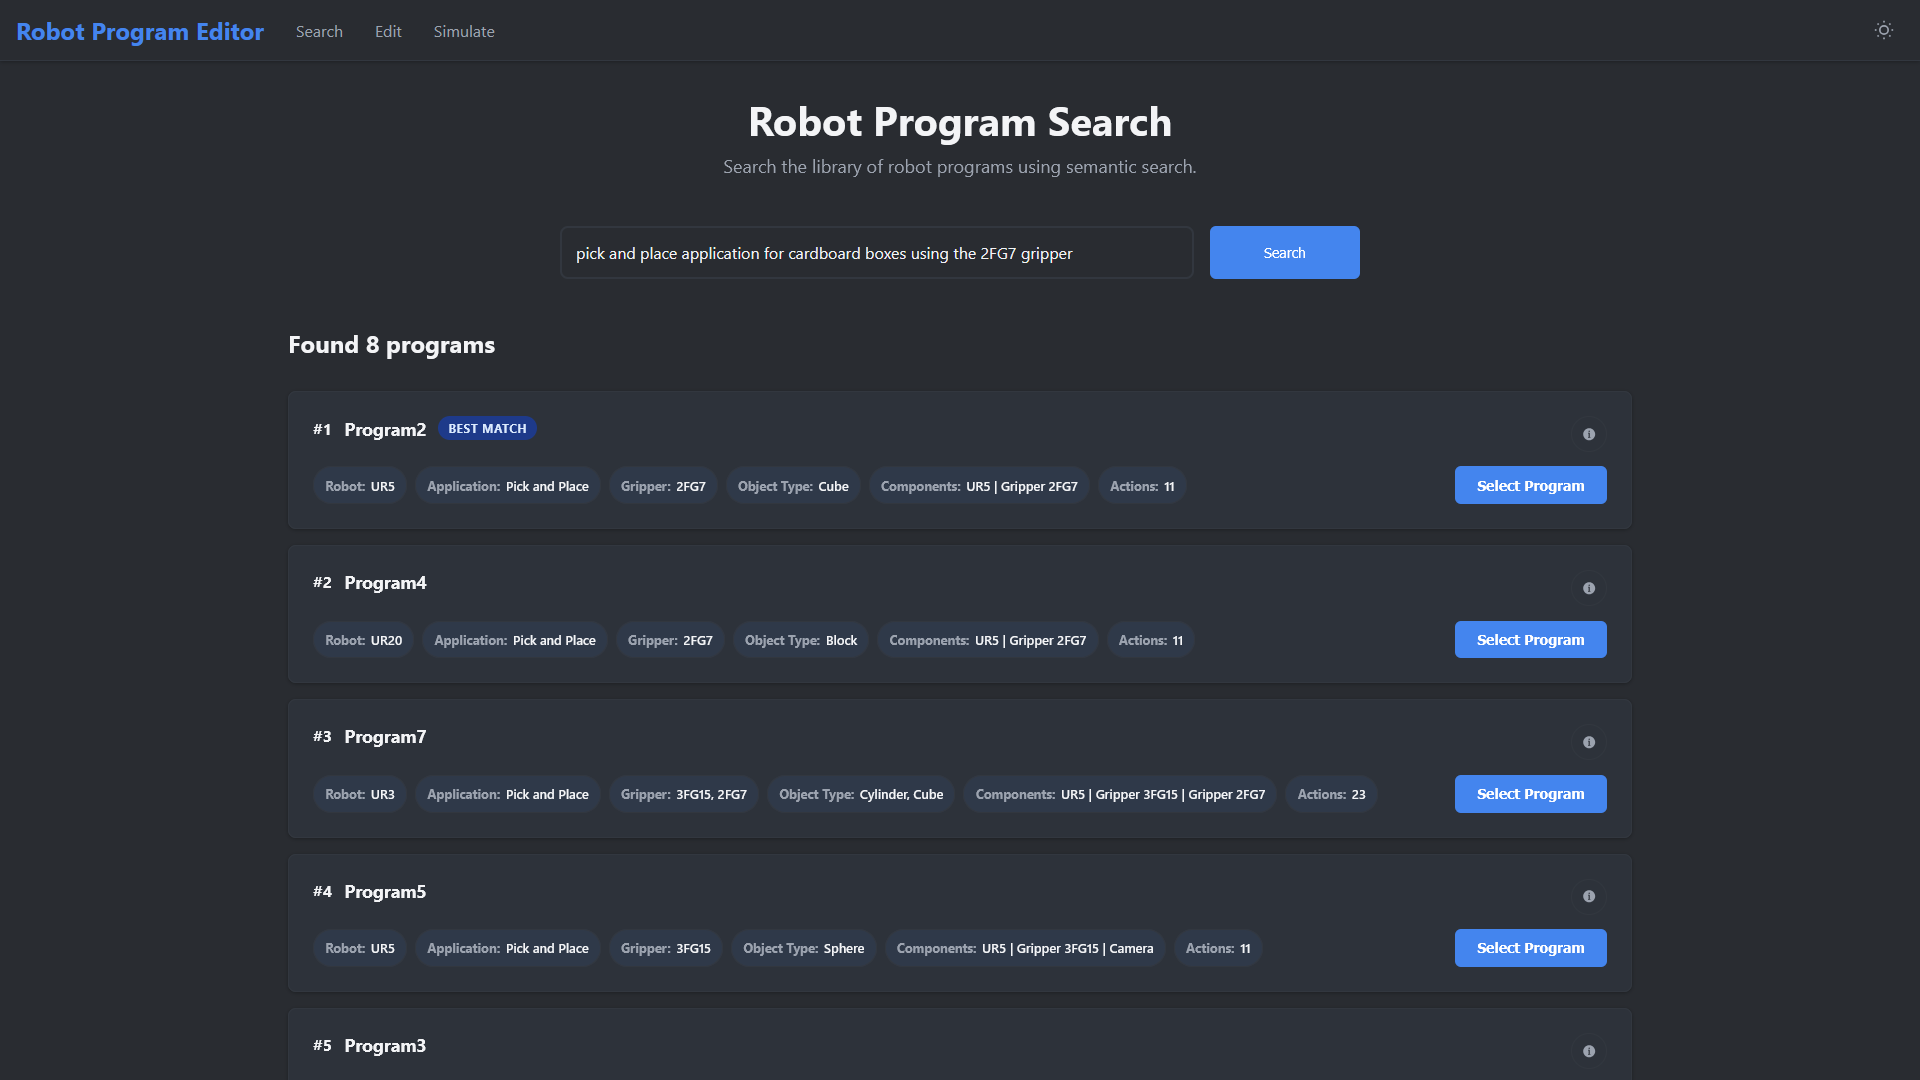
\includegraphics[width=\columnwidth]{media/search-tab.png}
	\caption{{Search page.}}
	\label{fig:implementation:search_tab}
\end{figure}

The editor tab (see Figure~\ref{fig:implementation:edit_tab}) is implemented in \texttt{Editor.jsx} as a three-panel layout using \texttt{react-resizable\-panels}. The left panel shows a generated program tree, the center panel hosts the Monaco code editor, and the right panel hosts the assistant chat. The layout is user-adjustable and persisted through the panel library so that panel widths remain consistent across revisits. This structure is designed to support assistant use directly during code inspection and editing, so program navigation, context selection, and chat interaction are available in one view. Program export is exposed through the editor menu.

\begin{figure}[H]
	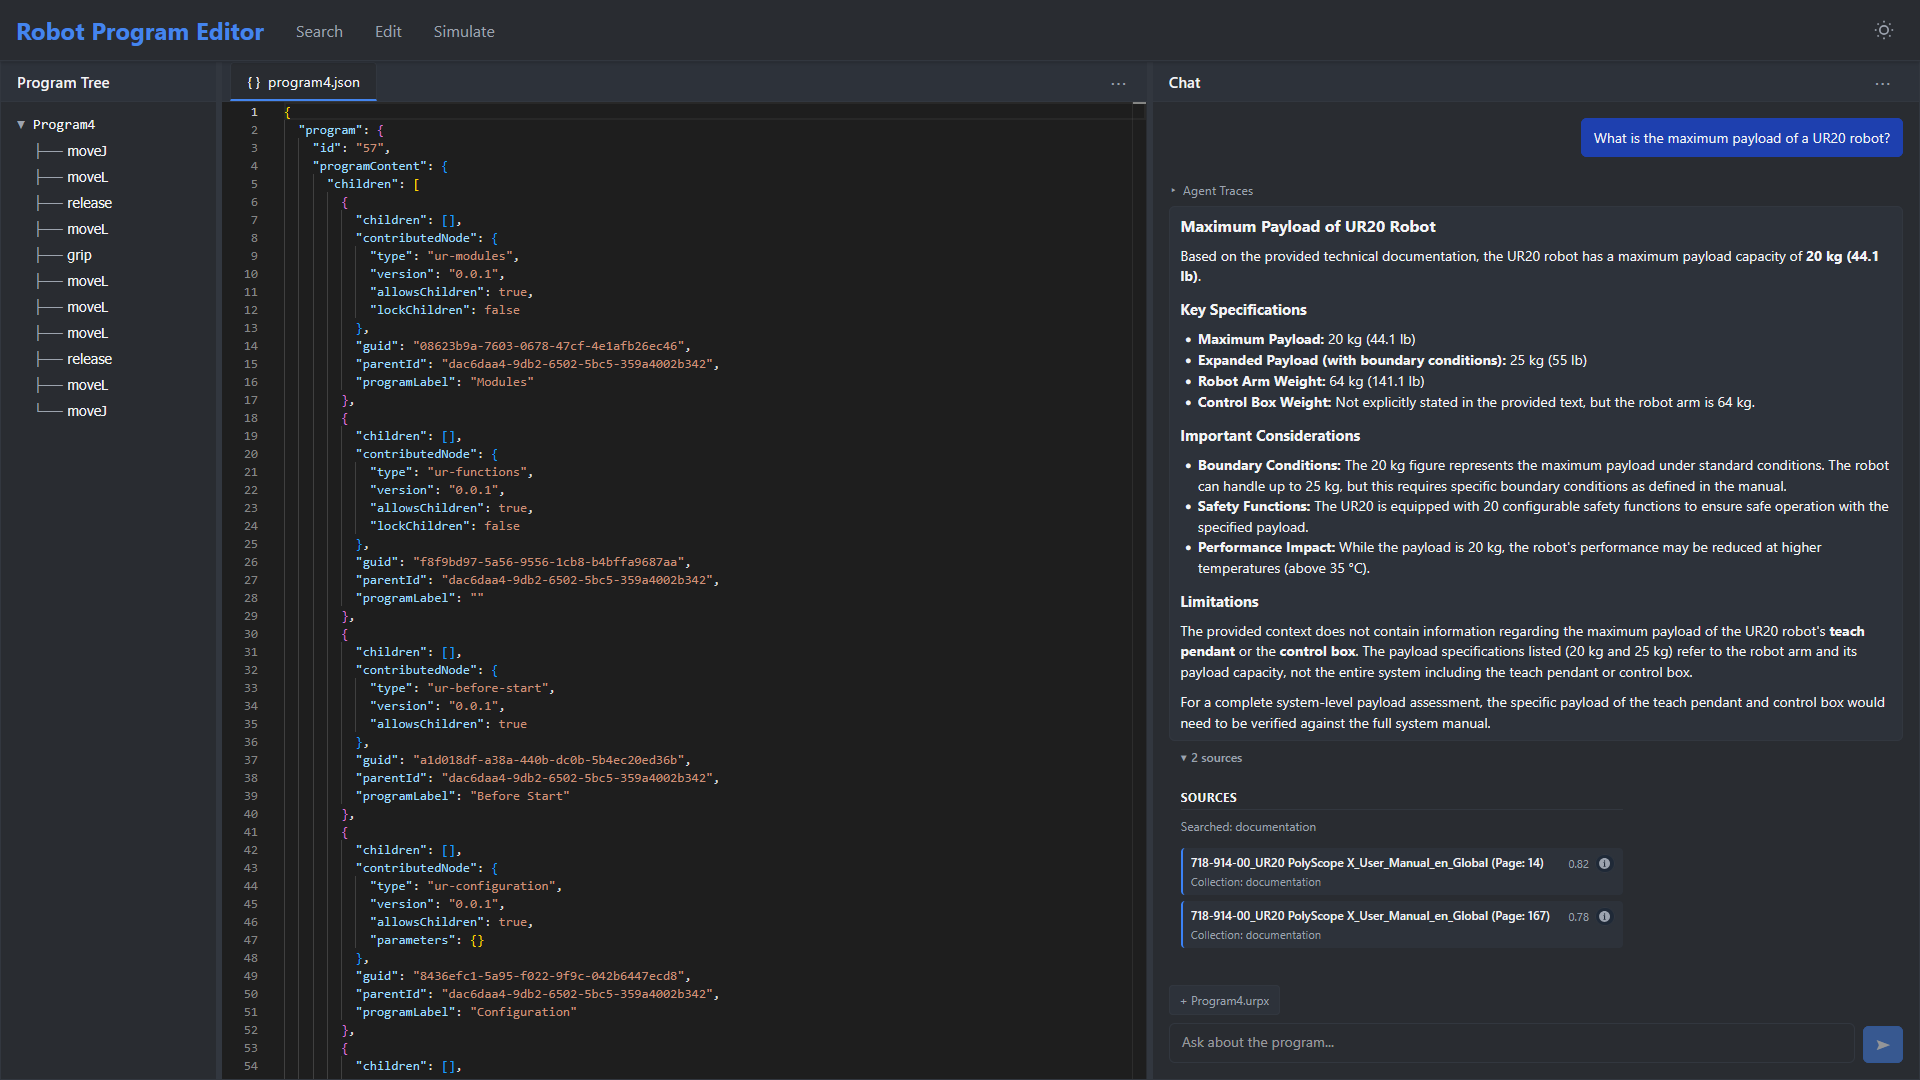
\includegraphics[width=\columnwidth]{media/edit-tab.png}
	\caption{{Edit page.}}
	\label{fig:implementation:edit_tab}
\end{figure}

The program tree is built client-side by parsing the loaded JSON and traversing the \texttt{ur-code} structure to collect action nodes. Action labels are derived from fields such as \texttt{moveType} and \texttt{action}. For each action, the frontend also resolves a corresponding line number in the editor by matching node \texttt{guid} values. Clicking a node in the program tree scrolls the code editor to the mapped location, places the cursor on that line, and centers the location in the viewport. This provides a way to navigate the program structure without needing to read through the raw code.

The chat panel, implemented in \texttt{RagChat.jsx}, supports contextual assistant interaction from within the editor workflow. The UI provides two equivalent ways to add program context: through the editor context menu and through the add-context button in the chat panel. If no code is highlighted, right-clicking in the editor and choosing the add-context action sends the entire program as context; the same full-program behavior is used when the chat-panel button is pressed without an active selection. If code is highlighted, only the highlighted line range is added. Users can attach one or more pending context snippets before asking a question, and each snippet is shown as a removable context field in the chat panel. Before transmission, \texttt{programContext.js} sanitizes the context by removing large \texttt{urscript} objects, as these are merely generated from the \texttt{.urpx} file, and so the assistant receives compact, higher-signal input.

During response generation, the interface shows live progress traces and then renders the final assistant reply as Markdown. Source details are exposed in expandable metadata blocks and hover tooltips, to provide transparency, and so users can inspect where retrieved evidence came from without leaving the editor. The chat menu also provides a clear-history action that resets both local chat state and server-side conversation memory.


\chapter{Evaluation} \label{chapter:evaluation}
This chapter describes the evaluation of the proposed approach. The evaluation is based on a user study, which is described in detail in Appendix \ref{appendix:evaluation-protocol}. The results of the user study are presented in section \ref{sec:evaluation:results}.

\section{Methodology} \label{sec:evaluation:methodology}
The evaluation was conducted as a controlled user study to assess the effect of the proposed system on robotic program comprehension and modification compared to the baseline workflow. The baseline condition used UR Studio, a browser-based PolyScope X simulation tool from Universal Robots with a visual programming interface similar to programming on the teach pendant.

The study addressed four research questions:
\begin{adjustwidth}{\indentWidthTwenty}{\indentWidthTwenty}
    \textit{\textbf{RQ1:} How does the proposed system influence the correctness of comprehension of robotic programs?}
\end{adjustwidth}
\begin{adjustwidth}{\indentWidthTwenty}{\indentWidthTwenty}
    \textit{\textbf{RQ2:} How does the proposed system influence the time required for comprehension of robotic programs?}
\end{adjustwidth}
\begin{adjustwidth}{\indentWidthTwenty}{\indentWidthTwenty}
    \textit{\textbf{RQ3:} How does the proposed system influence the correctness of modification and reuse of robot programs?}
\end{adjustwidth}
\begin{adjustwidth}{\indentWidthTwenty}{\indentWidthTwenty}
    \textit{\textbf{RQ4:} How does the proposed system influence the time required in the modification and reuse of robot programs?}
\end{adjustwidth}

\subsection{Study Design}
The experiment used a within-subjects design in which each participant completed tasks in both conditions (baseline and proposed system). To reduce order effects, condition order was counterbalanced across participant groups. In addition, two distinct task sets were used across conditions so that participants could not directly transfer solutions from one condition to the other.

Each condition consisted of two phases:
\begin{itemize}
    \item \textbf{Exploration phase:} Participants first familiarized themselves with the assigned condition through guided walkthroughs and practice.
    \item \textbf{Task phase:} Participants then completed comprehension and modification tasks used for evaluation.
\end{itemize}

\subsection{Participants and Pre-Study Survey}
Participants were recruited from potential users of the system, including robotics engineers and programmers with experience in robotic systems, sourced from industry and academia. Before starting the tasks, each participant completed a pre-study survey capturing self-reported robotic programming experience and familiarity/use of AI assistants.

\subsection{Task Design}
The task set was designed to reflect realistic work with robot programs and to evaluate both understanding and change implementation.

Comprehension tasks required participants to inspect programs and answer multiple-choice questions on key actions, action order, waypoint order, URCap usage, gripper usage, and the overall application. Participants also rated their confidence in their own comprehension on a 1--5 Likert scale.

Modification tasks required participants to apply concrete changes to existing programs. Across the two task sets, these changes included modifying speed, changing movement type, switching waypoints between move actions, enabling blend movement, and adding a wait action.

\subsection{Metrics}
The evaluation combined quantitative and qualitative metrics.

Quantitative metrics were:
\begin{itemize}
    \item \textbf{Correctness of comprehension:} Number of correctly answered comprehension questions.
    \item \textbf{Time for comprehension:} Time required to complete comprehension tasks.
    \item \textbf{Correctness of modifications:} Degree to which implemented changes satisfied task requirements, including preservation of existing functionality where applicable.
    \item \textbf{Time for modifications:} Time required to complete modification tasks.
    \item \textbf{Confidence ratings:} Post-task confidence on a 1--5 Likert scale.
\end{itemize}

For comprehension, correctness was based on correct multiple-choice responses. For modification, correctness was evaluated against predefined expected outcomes, with partial correctness assigned when only part of the required change was achieved.

Qualitative metrics were:
\begin{itemize}
    \item System-wide user feedback on usability, usefulness, and challenges.
    \item Feedback specifically on LLM-assisted functionality (user perceived response quality, relevance, clarity, and factual correctness).
    \item Observational data on participant behavior, interactions, and encountered difficulties.
\end{itemize}

\subsection{Procedure}
For each participant, the study proceeded as follows: (1) pre-study survey, (2) completion of the two conditions in counterbalanced order, with an exploration phase followed by a task phase in each condition, and (3) post-study questionnaire.

After completing the tasks, participants provided post-study ratings on ease of use, perceived usefulness, confidence in comprehension and modification for both conditions, and assessments of LLM-generated comprehension responses and modification suggestions. Open-ended questions captured perceived challenges, improvement suggestions, and willingness to use the proposed system in future robotic programming work.

This procedure enabled direct comparison of correctness, completion time, confidence, and user experience between the proposed system and the baseline approach while controlling for learning effects through counterbalancing and distinct task sets.


\section{Results} \label{sec:evaluation:results}
This section presents the results of the user study collected from five participants. Condition A denotes the baseline (UR Studio) and condition B denotes the system proposed in this thesis. The raw evaluation results used in this analysis are provided in Appendix \ref{appendix:evaluation-data}.

The evaluation was performed on with the following hardware; CPU: AMD Ryzen 7 9800X3D, RAM: 32GB DDR5, GPU: NVIDIA RTX 5070 Ti. Language models as described in Chapter \ref{chapter:implementation}.

\subsection{Data Preparation}
Correctness scores for comprehension tasks were scored as 1 for correct and 0 for incorrect answers.

\textbf{Comprehension Task (CT):}
\begin{itemize}
    \item \textbf{CT-1 (Key Actions)}
    \item \textbf{CT-2 (Action Sequence)}
    \item \textbf{CT-3 (Waypoint Sequence)}
    \item \textbf{CT-4 (URCap Usage)}
    \item \textbf{CT-5 (Gripper Type)}
    \item \textbf{CT-6 (Overall Application)}
\end{itemize}

For modification tasks, correctness was scored based on the degree to which the implemented change met the task requirements, with partial credit assigned for partially correct solutions. All programs were verified with UR Studio and manual code analysis. The scoring rubric for modification tasks was as follows:

\textbf{Modification Task (MT) Scoring Rubric:}
\begin{itemize}
    \item \textbf{MT-1 (Speed Modification):} Correctly changing the "optiMoveSpeed" parameter scores 1 point; changing the other speed parameter scores 0 points.
    \item \textbf{MT-2 (Movement Type Change):} Changing the "moveType" from moveL to moveJ or vice versa scores 1 point; no change or an incorrect change scores 0 points.
    \item \textbf{MT-3 (Waypoint Switch):} Correctly switching the positions of the waypoints in the correct order and with the correct move type and parameters scores 1 point; any other change scores 0 points.
    \item \textbf{MT-4 (Blend Enablement):} Enabling blend without specifying a blend radius scores 0.5 points; enabling blend with a specified blend radius scores 1 point; not enabling blend or incorrect changes score 0 points.
    \item \textbf{MT-5 (Wait Node Addition):} Inserting a wait node with the correct structure and in the correct spot scores 1 point; any other change scores 0 points.
\end{itemize}

\subsection{Pre-Study Participant Profile}
The pre-study responses provide context for interpreting the task results. Regarding robotics-programming experience, three participants reported \textit{Intermediate} experience (60\%), one reported \textit{Beginner} (20\%), and one reported \textit{Advanced} (20\%). Thus, all participants had at least some experience with robotic programming, with a majority at the self-proclaimed intermediate level.

For general software-development work, four participants reported frequent AI-assistant usage: two \textit{Always} (40\%) and two \textit{Often} (40\%), while one reported \textit{Sometimes} (20\%). All participants where familiar with AI assistants for software development, with the majority using them frequently.

All participants were positively inclined toward AI assistance for robot program development before the study: three selected \textit{Strongly agree} (60\%) and two selected \textit{Agree} (40\%) for the statement that they would use an AI assistant for developing robot programs.

The participants were asked to explain their reasoning to why or why not to use AI for robot program development. Participants primarily emphasized productivity and acceleration benefits, such as reducing integration time, receiving solution suggestions during development, and faster drafting of robot programs. One participant also highlighted a potential trade-off, noting concern that heavy AI use could reduce deeper understanding of the robot program if the assistant "does everything". Overall, pre-study attitudes suggest optimism: participants expected AI assistance to be useful, while still recognizing possible impacts on learning depth.


\subsection{Quantitative Results}
All participants completed both conditions. Some participants gave up on certain modification subtasks, with one value marked \textit{DNF} (Did Not Finish) in condition A and four values marked \textit{DNF} in condition B.

For consistency, all reported task-time means and medians are computed from completed tasks only, while \textit{DNF} cases are accounted for separately through the task-completion-rate metric.

For correctness, two metrics are reported: (1) completed-only correctness (excluding \textit{DNF} values), and (2) DNF-inclusive correctness where \textit{DNF} is treated as incorrect. In the summary table, DNF-inclusive values are shown in parentheses after completed-only values.

The participants had the option to use the AI assistant in condition B as much or as little as they wanted. Some participants only used the assistant when they were blocked, while others used it more proactively to explore functionality. Thus, the subjective assistant usage is an important factor to consider when interpreting the results.

Assistant interaction logs were collected for 43 assistant requests across all participants. Each log includes a session start and end timestamp, where start is the user query and end is the assistant's final response. The manually extracted file \texttt{assistant\_task\_extraction.csv} links each assistant session with a \texttt{task\_id} label.

Table \ref{tab:evaluation:key-results} summarizes the primary quantitative outcomes.

\begin{table}[H]
    \centering
    \begin{tabular}{p{7cm}cc}
        \toprule
        \textbf{Metric}                          & \textbf{Baseline (A)} & \textbf{Proposed (B)} \\
        \midrule
        Comprehension correctness                & 1.00 (1.00)           & 0.97 (0.97)           \\
        Modification correctness                 & 1.00 (0.96)           & 0.60 (0.50)           \\
        Comprehension time, mean [min]           & 3.25                  & 6.97                  \\
        Comprehension time, median [min]         & 2.62                  & 6.18                  \\
        Modification time, mean [min]            & 4.85                  & 9.81                  \\
        Modification time, median [min]          & 4.03                  & 12.53                 \\
        Comprehension task completion rate       & 1.00                  & 1.00                  \\
        Modification task completion rate        & 0.96                  & 0.84                  \\
        Confidence in comprehension (Likert 1-5) & 4.40                  & 2.00                  \\
        Confidence in modification (Likert 1-5)  & 3.40                  & 2.60                  \\
        \bottomrule
    \end{tabular}
    \caption{Quantitative result summary across baseline (A) and proposed (B) conditions. For correctness rows, values in parentheses are DNF-inclusive (\textit{DNF}=incorrect). Time means/medians are based on completed tasks only; \textit{DNF} cases are reflected in the completion-rate rows.}
    \label{tab:evaluation:key-results}
\end{table}

\subsubsection*{RQ1: How does the proposed system influence the correctness of comprehension of robotic programs?}
The proposed system had a negligible effect on comprehension correctness. Scores were near-perfect in both conditions: baseline reached proportion correct of 1.00 (30/30), and the proposed condition achieved 0.97 (29/30). The single incorrect response in the proposed condition occurred on the action-sequence task, where one participant chose the wrong action chain. This is the strongest positive result for the proposed system. Even with the raw \texttt{.urpx} representation of the program, participants were generally able to identify key actions, action order, waypoint order, URCap usage, gripper type, and overall program application. The structured JSON view, combined with the program tree navigation panel and assistant explanations, was sufficient to support correct program comprehension at the level required by these tasks.

\subsubsection*{RQ2: How does the proposed system influence the time required for comprehension of robotic programs?}
The proposed system increased wall-clock comprehension time. Mean comprehension time per participant increased from 3.25 for the baseline to 6.97 minutes for the proposed system, a roughly 2x increase. The median followed the same pattern, increasing from 2.62 to 6.18 minutes. The paired Wilcoxon test gave $p = 0.31$ ($n=5$), and Cliff's delta was $\delta = +0.52$. This means that, with this sample size, the statistical test does not indicate a reliable difference at conventional significance levels, but the effect-size estimate suggests a practically large shift toward longer comprehension times in the proposed condition.

When assistant wait time is subtracted, the interpretation changes. The mean active comprehension time (subtracting assistant wait time) in the proposed condition was 4.07 minutes, and the effect size dropped to $\delta = +0.20$. This indicates that most of the observed wall-clock increase came from assistant latency rather than substantially slower user work.

The task-level breakdown in Figure \ref{fig:evaluation:time-by-task-ai-comp} is consistent with this interpretation when the proposed mean is split by assistant use. For CT-1, CT-2, CT-4, and CT-5, the proposed \textit{without-assistant} means were close to baseline (CT-1: $-16.5$ s, CT-2: $-11.9$ s, CT-4: $+0.7$ s, CT-5: $+3.6$ s), and CT-6 was faster than baseline ($-47.7$ s). In contrast, the proposed \textit{with-assistant} means were markedly higher than baseline on most tasks (CT-1: $+186.0$ s, CT-2: $+175.6$ s, CT-3: $+201.0$ s, CT-4: $+150.5$ s, CT-5: $+61.6$ s). CT-3 remained slower even without assistant use ($+27.5$ s), suggesting additional task-intrinsic difficulty for waypoint-sequence tracing in the raw JSON representation.

Assistant logs show the same pattern for comprehension-task sessions. Across 24 comprehension-linked sessions, mean response time was 40.94 s (median 40.94 s). Mean embedding time was 4.16 s per call. The 5-call retrieval cap was reached in 8.3\% of comprehension sessions (2/24), and those capped sessions averaged 62.48 s. Together, this suggests that reducing assistant latency is likely to reduce a large portion of the comprehension-time penalty.

\begin{figure}[H]
    \centering
    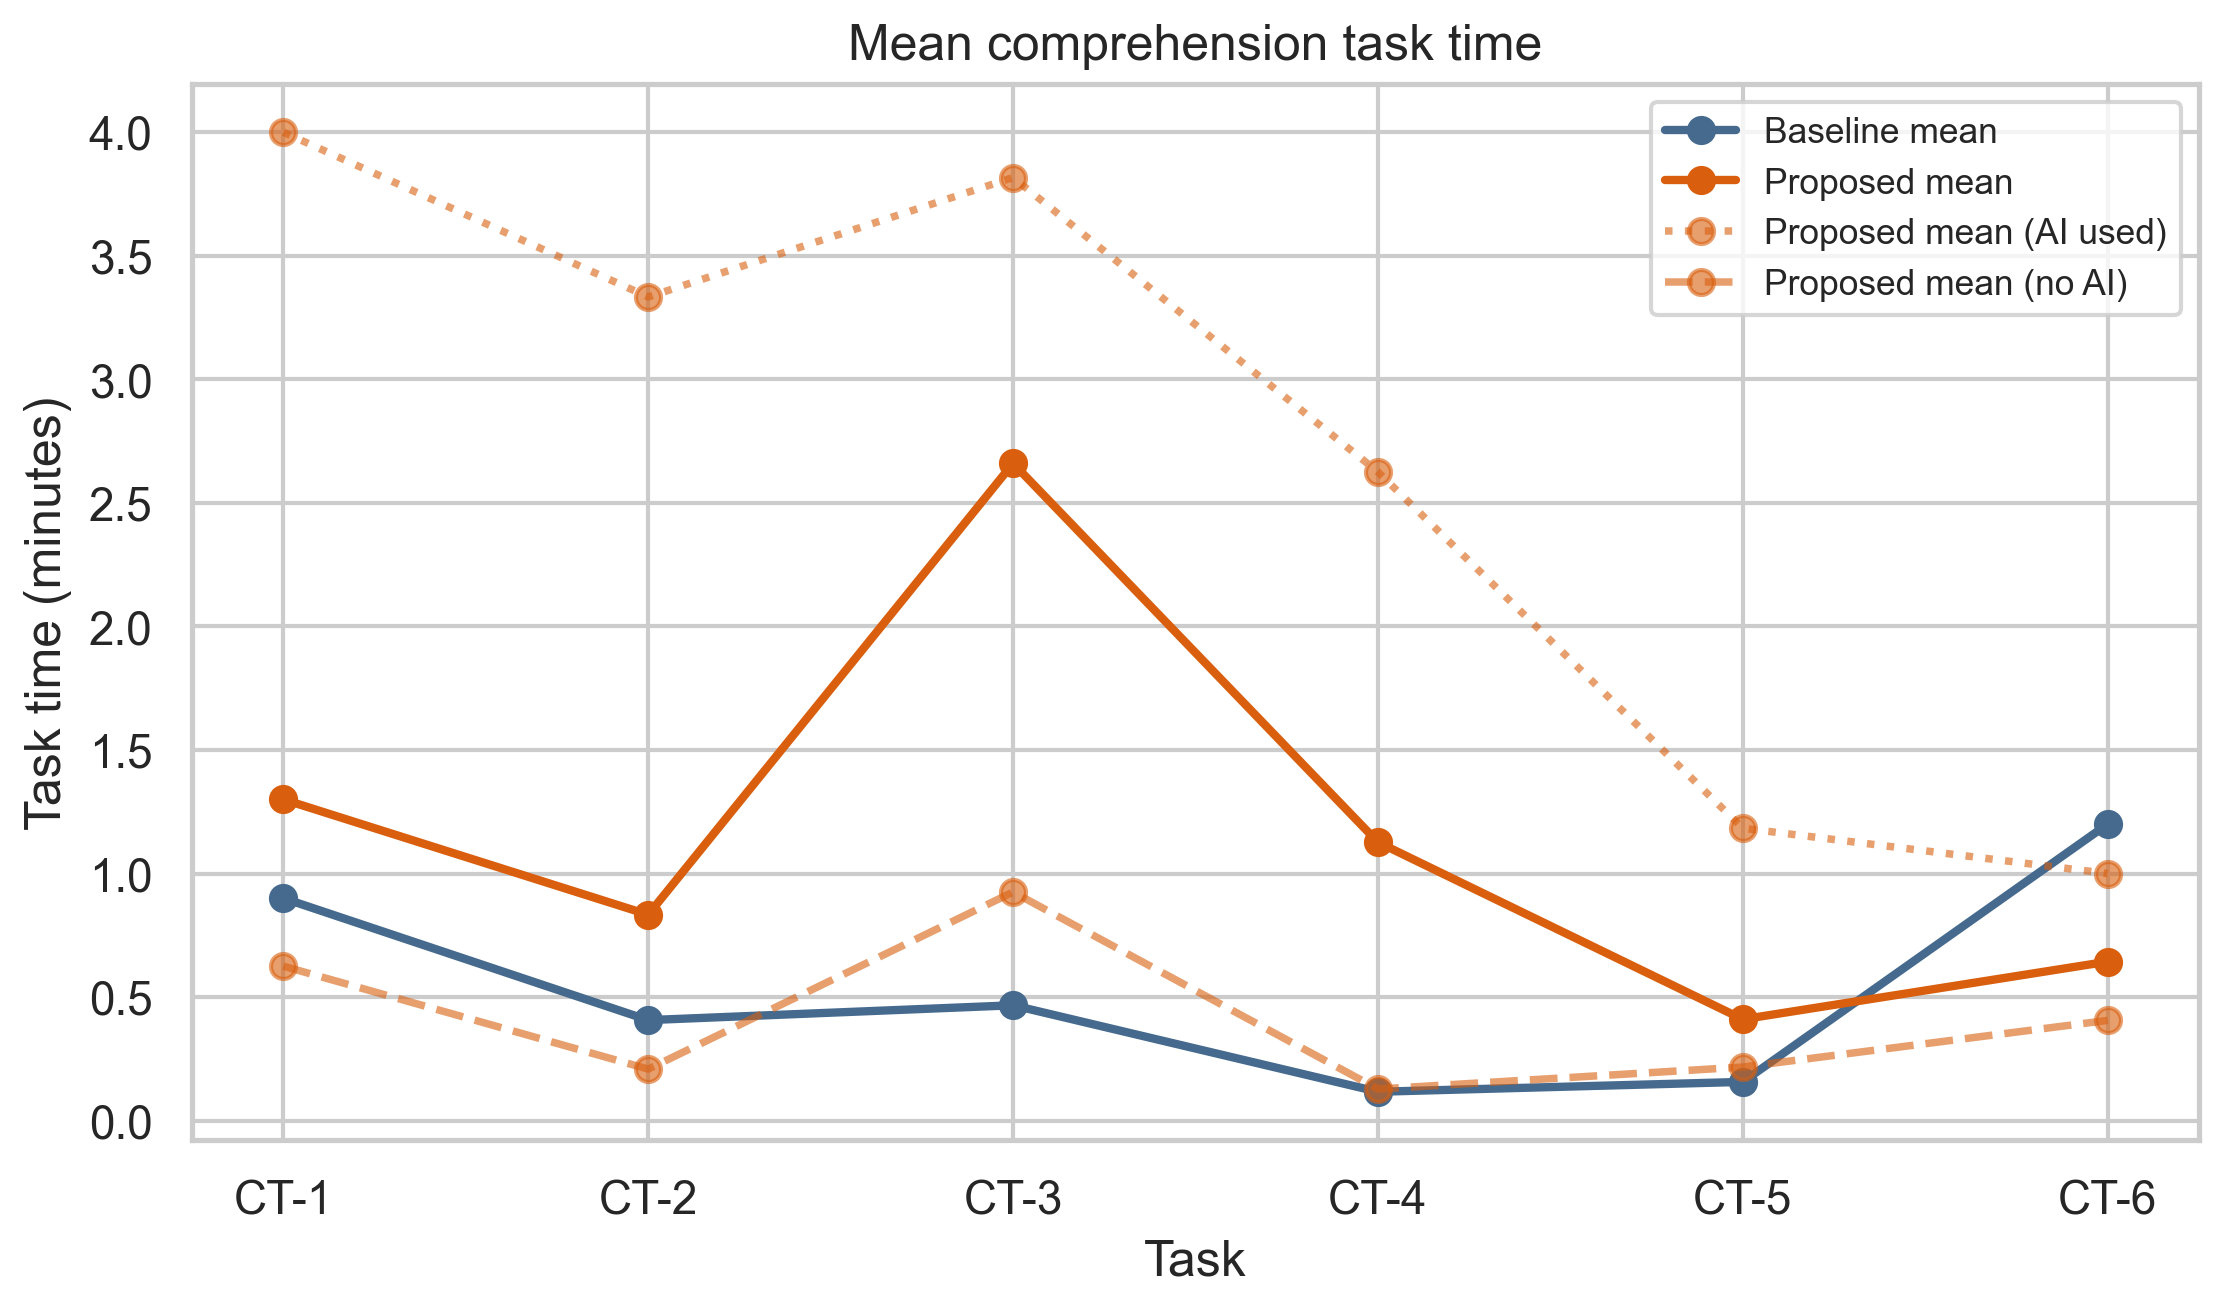
\includegraphics[width=0.88\columnwidth]{media/evaluation/time_by_task_order_with_ai_use_comprehension.png}
    \caption{Mean comprehension task (CT) time by task (CT-1--CT-6), comparing baseline (A) and proposed (B), with condition B split by whether the assistant was used on the task.}
    \label{fig:evaluation:time-by-task-ai-comp}
\end{figure}

% Figure \ref{fig:evaluation:time-participant-comp} shows the comprehension time by tasks for each participant (baseline dashed, proposed solid).

% \begin{figure}[H]
%     \centering
%     \includegraphics[width=0.88\columnwidth]{media/evaluation/task_time_per_participant_comprehension.png}
%     \caption{Comprehension task time by participant across tasks (baseline dashed, proposed solid).}
%     \label{fig:evaluation:time-participant-comp}
% \end{figure}

\subsubsection*{RQ3: How does the proposed system influence the correctness of modification and reuse of robot programs?}
The proposed system reduced modification correctness substantially relative to the baseline. In baseline, completed-only correctness was 1.00 (24/24), with DNF-inclusive correctness of 0.96 (24/25). In the proposed condition, completed-only correctness was 0.60 (12.5/21), and DNF-inclusive correctness was 0.50 (12.5/25). At the aggregate level, this is a substantial regression.

The aggregate, however, obscures considerable variation across modification task types. The five modification tasks behaved very differently. MT-2 (movement type change) remained perfect in both conditions (1.00 vs. 1.00). MT-3 (waypoint switch) showed a smaller decrease (1.00 vs. 0.80). In contrast, MT-1 (speed modification) dropped to 0.20, MT-4 (blend enablement) to 0.50, every participant scored partial credit, the full mark required also specifying the blend radius, which no participant did. MT-5 (wait node addition) dropped to 0.00.

This pattern points to a structural failure rather than a general inability to modify programs with the proposed system. Participants performed relatively well when updating existing values (MT-2 and MT-3), but struggled on tasks requiring parameter disambiguation (MT-1) and node insertion (MT-4 and MT-5) in the raw \texttt{.urpx} structure.

\subsubsection*{RQ4: How does the proposed system influence the time required in the modification and reuse of robot programs?}
The proposed system also increased modification time substantially. Mean modification time per participant increased from 4.85 to 9.81 minutes, and the median increased from 4.03 to 12.53 minutes. The paired Wilcoxon test gave $p = 0.44$ ($n=5$), with a large effect size ($\delta = +0.52$). Completion rate also dropped (0.96 baseline vs. 0.84 proposed). As for comprehension, the Wilcoxon result is not statistically significant with $n=5$, but Cliff's delta indicates a large directional effect toward longer modification times in the proposed condition.

Unlike comprehension, this penalty remained large after subtracting assistant wait time. Mean active modification time in the proposed condition was 8.04 minutes, and the active-time effect size remained $\delta = +0.52$. This indicates that modification work itself was slower in the proposed workflow, not only delayed by assistant latency.

The task-level breakdown in Figure \ref{fig:evaluation:time-by-task-ai-mod} shows the same pattern when the proposed mean is split by assistant use. The proposed \textit{without-assistant} means were close to baseline for MT-1, MT-2, and MT-4 (MT-1: $+5.7$ s, MT-2: $+3.6$ s, MT-4: $+4.6$ s), while MT-3 was faster than baseline ($-187.0$ s). In contrast, the proposed \textit{with-assistant} means were higher than baseline across all modification tasks (MT-1: $+246.9$ s, MT-2: $+34.6$ s, MT-3: $+130.8$ s, MT-4: $+164.6$ s, MT-5: $+82.4$ s). For MT-5, all completed proposed-condition attempts used the assistant, so there is no corresponding without-assistant mean.

Assistant logs for modification tasks indicate a heavier latency profile than in comprehension. Across 19 modification-linked sessions, mean response time was 55.57 s (median 46.19 s). Mean embedding time was 4.12 s per call. The 5-call retrieval cap was reached in 26.3\% of modification sessions (5/19), and those capped sessions averaged 82.07 s. This is consistent with the larger remaining modification-time penalty, where assistant-related delay is more prominent and more variable.

\begin{figure}[H]
    \centering
    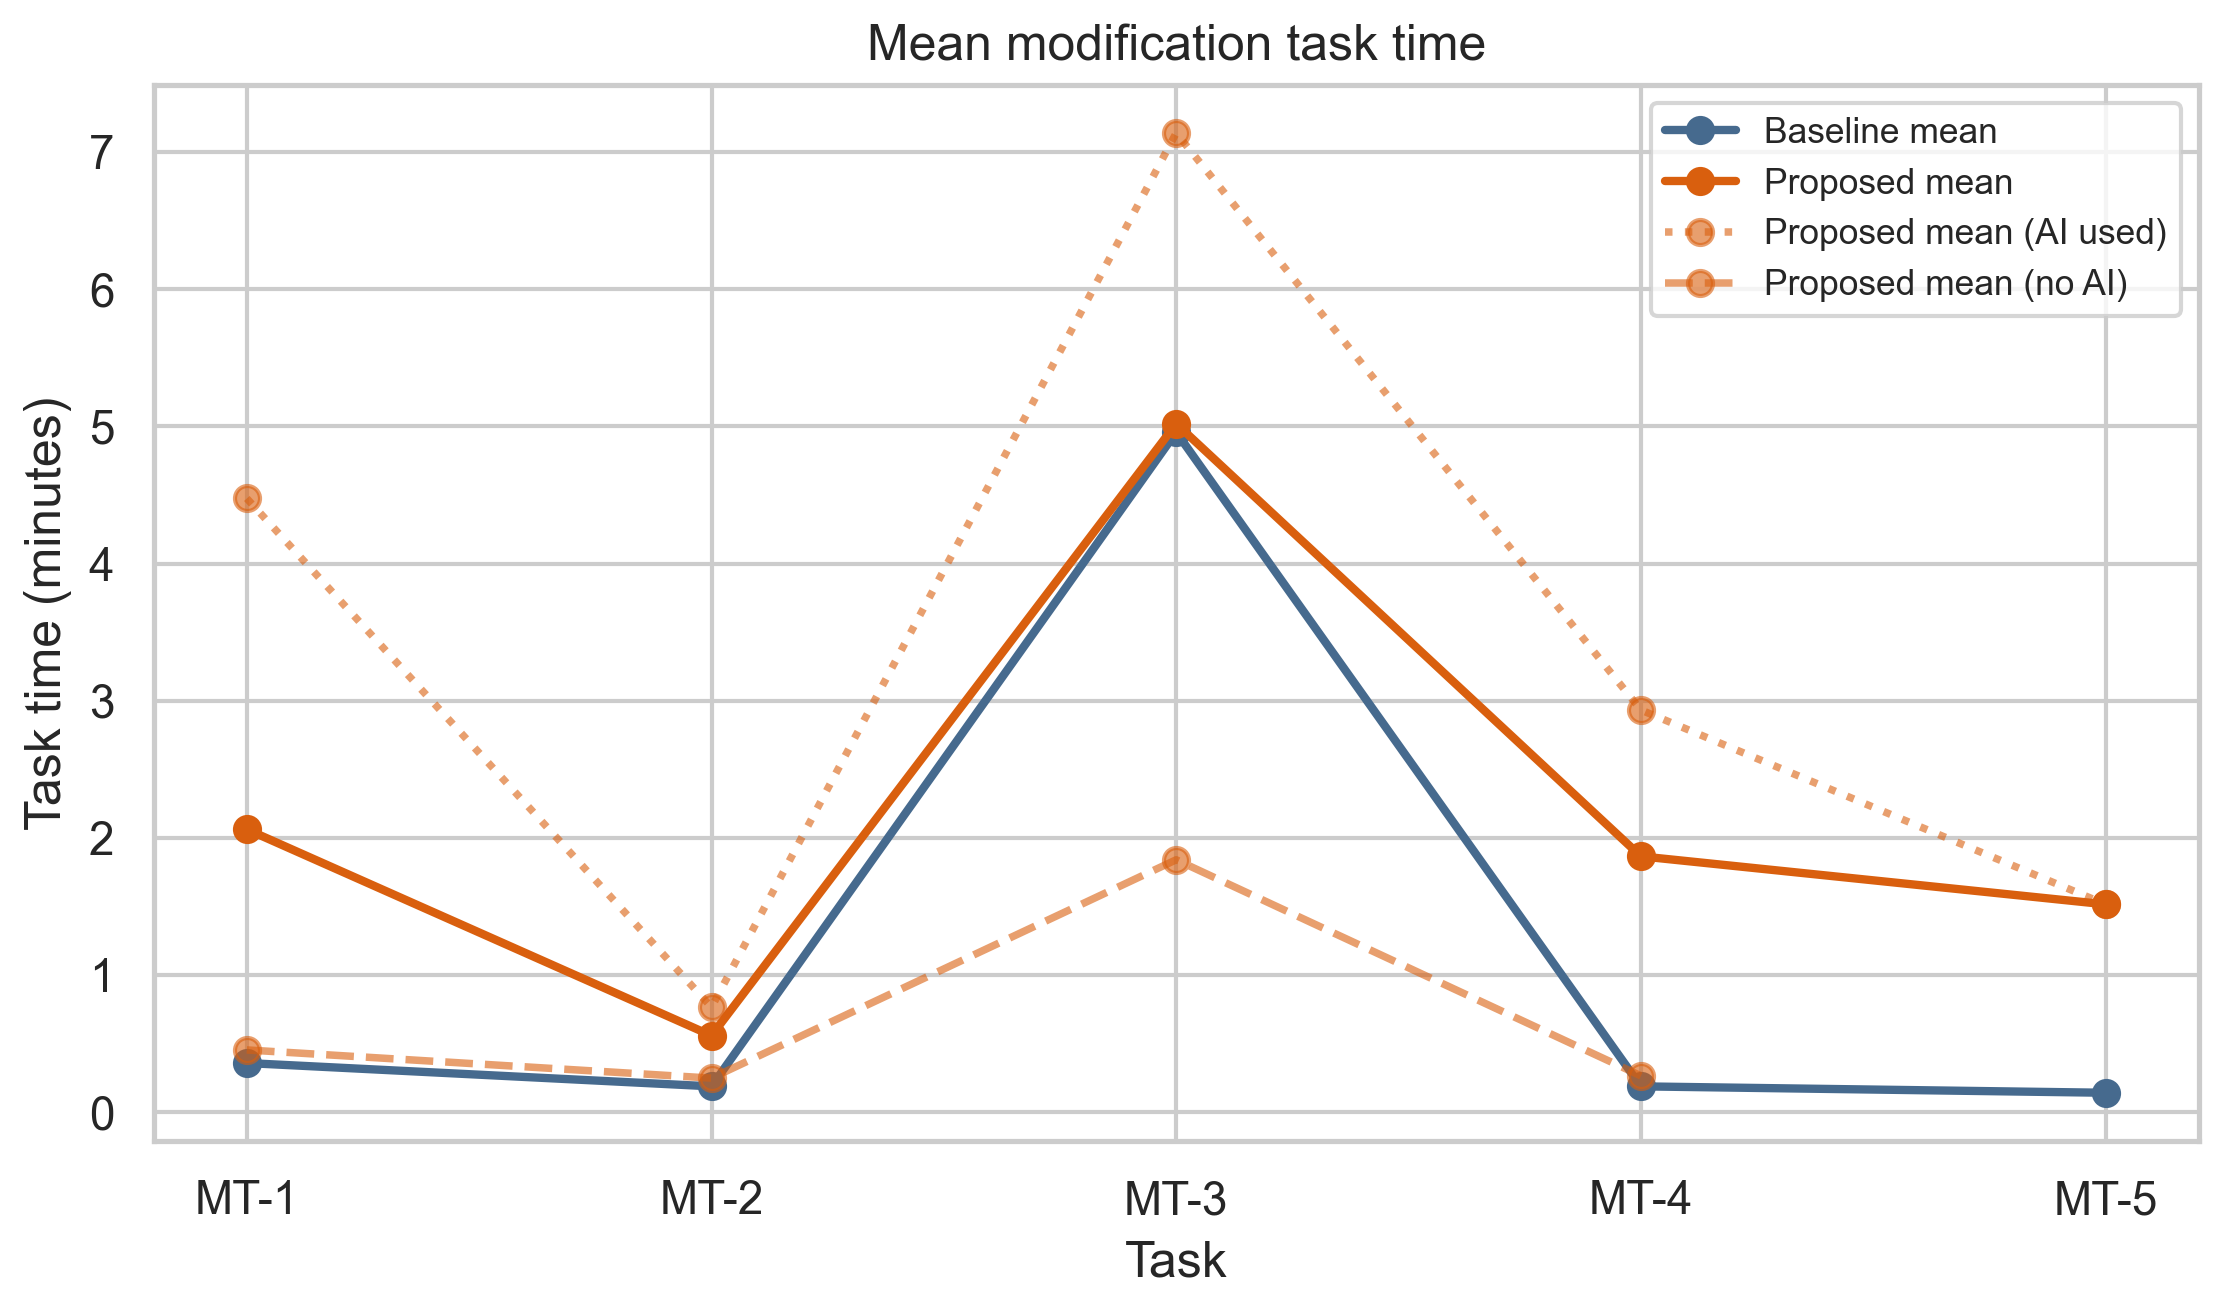
\includegraphics[width=0.88\columnwidth]{media/evaluation/time_by_task_order_with_ai_use_modification.png}
    \caption{Mean modification task (MT) time by task (MT-1 -- MT-5), comparing baseline (A) and proposed (B), with condition B split by whether the assistant was used on the task.}
    \label{fig:evaluation:time-by-task-ai-mod}
\end{figure}

% \begin{figure}[H]
%     \centering
%     \includegraphics[width=0.88\columnwidth]{media/evaluation/task_time_per_participant_modification.png}
%     \caption{Modification task (MT-1--MT-5) time by participant (baseline dashed, proposed solid).}
%     \label{fig:evaluation:time-participant-mod}
% \end{figure}

\subsubsection*{Confidence}
Self-reported confidence was lower with the proposed system than with baseline for both comprehension (2.00 vs. 4.40) and modification (2.60 vs. 3.40), as shown in Figure \ref{fig:evaluation:confidence}.

Notably, there is a comprehension-confidence gap. Participants reported very low confidence in the proposed condition (2.00), even though comprehension correctness remained high (0.97, with only one incorrect response across all comprehension answers). This suggests that participants were often unsure about their answers while working in the raw \texttt{.urpx} representation, even when they ultimately answered correctly. In contrast, modification shows both lower confidence and substantially lower correctness, indicating that participants' lower confidence in modification more closely reflected actual difficulties.

\begin{figure}[H]
    \centering
    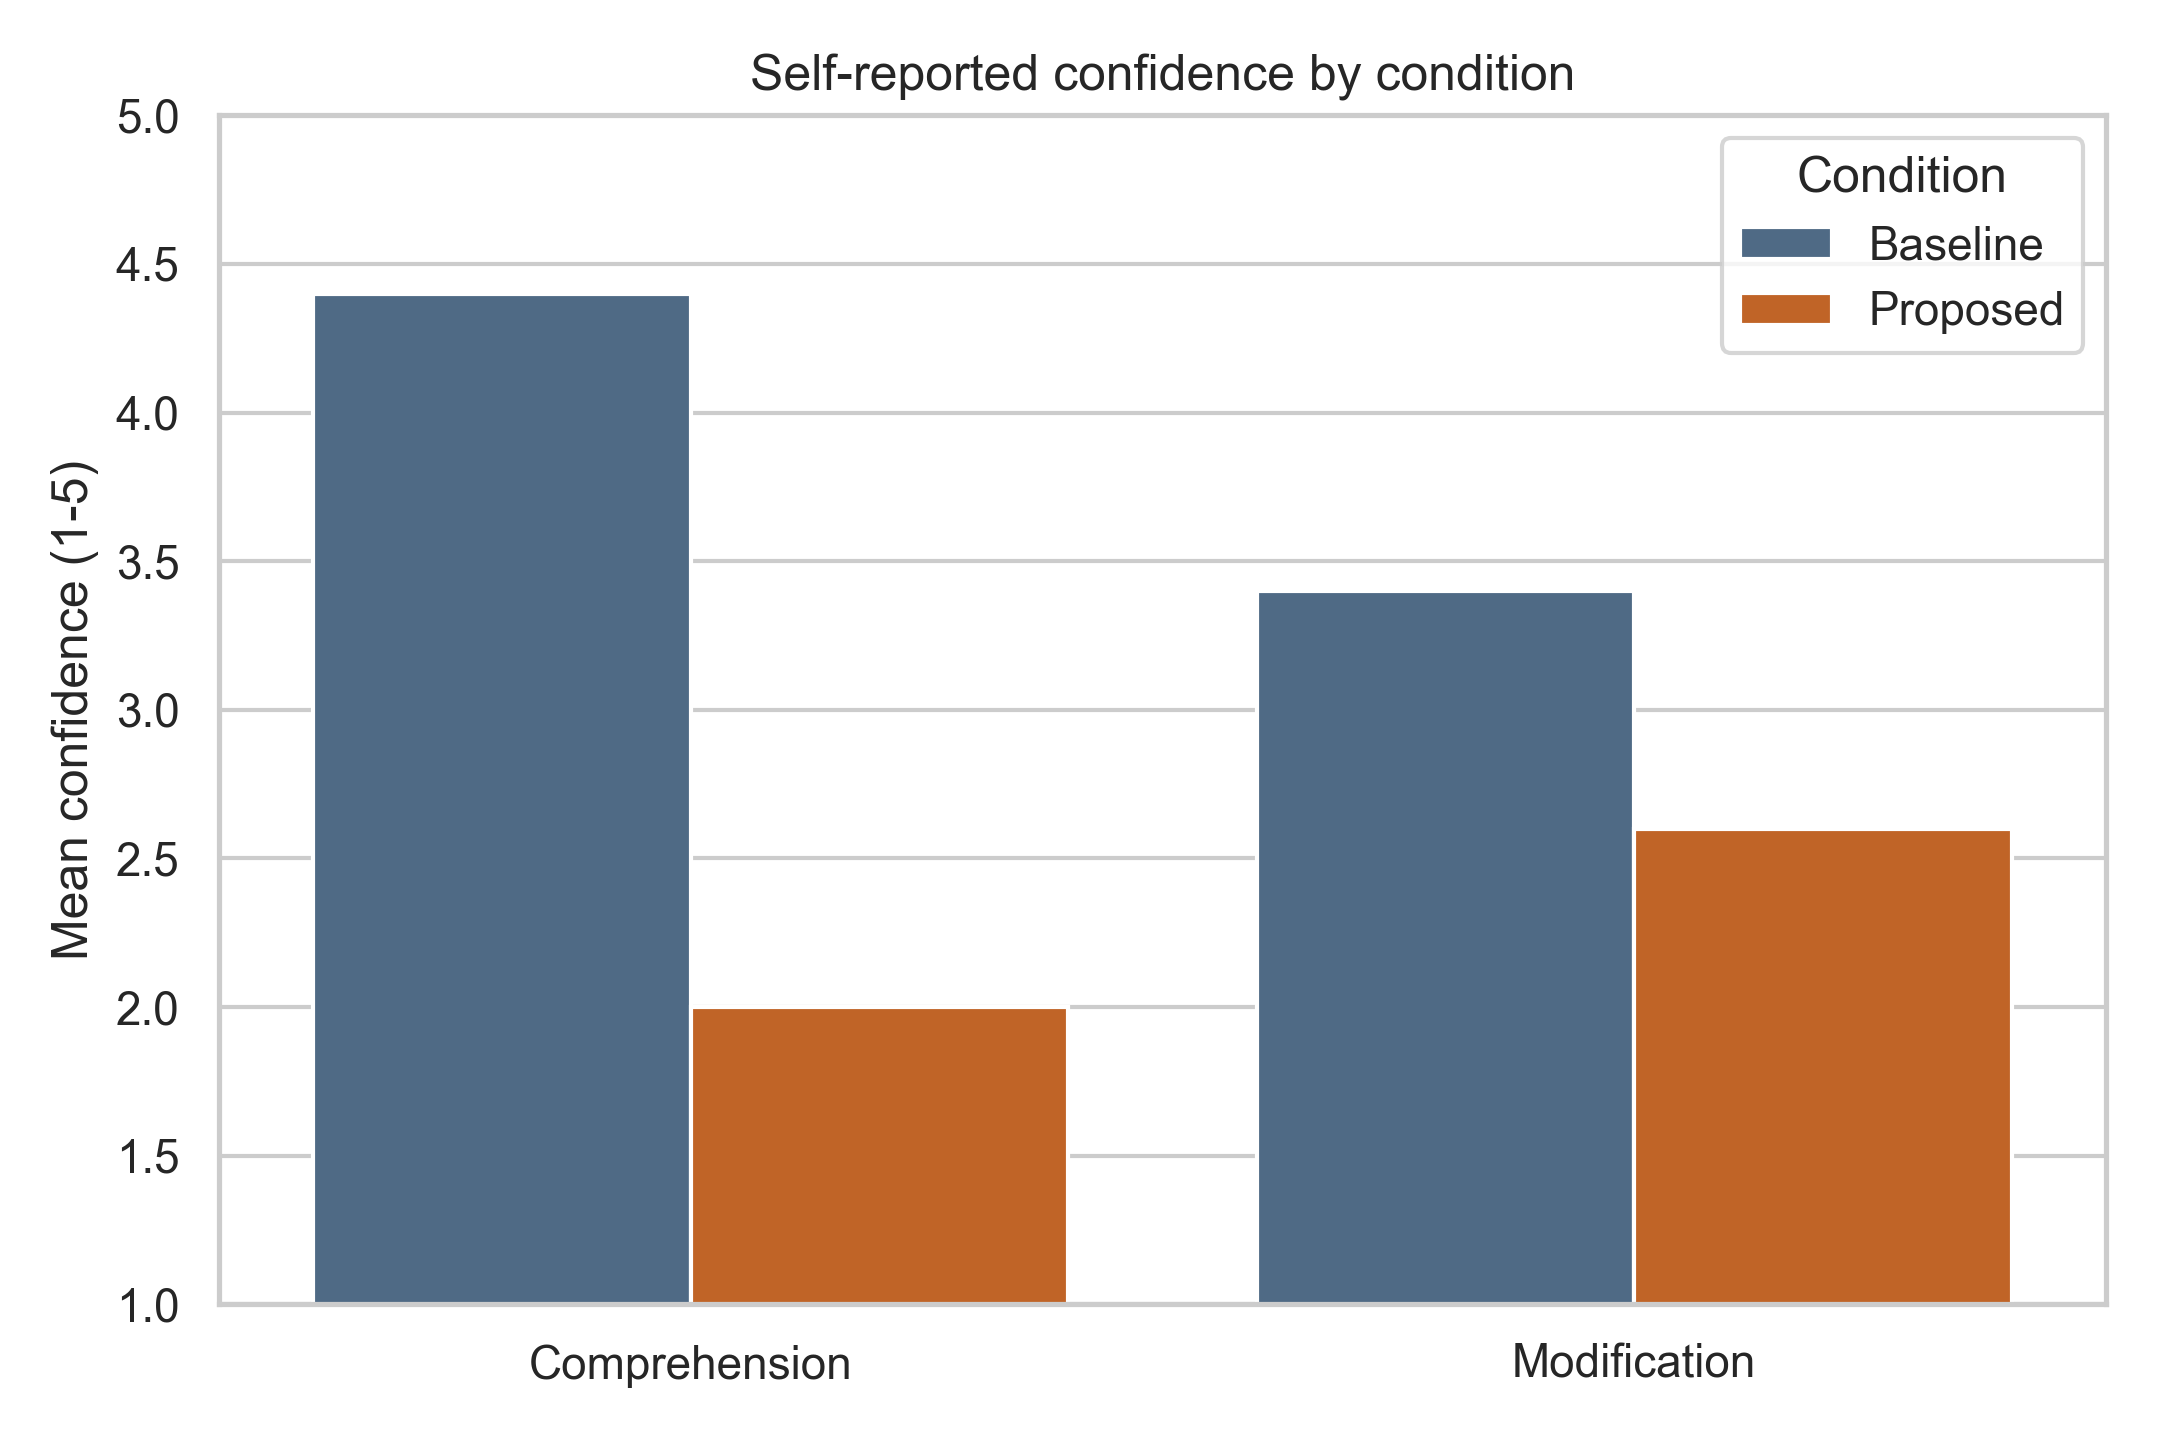
\includegraphics[width=0.62\columnwidth]{media/evaluation/confidence_by_condition.png}
    \caption{Mean self-reported confidence (Likert 1-5) for comprehension and modification by condition.}
    \label{fig:evaluation:confidence}
\end{figure}


\subsubsection*{AI Assistant Usage and Latency}
The AI assistant was used in 26 of 55 possible task opportunities in condition B (47.3\%). Usage varied by task and was highest for MT-5 (100\% of participants). The next-highest usage was 60\% on CT-3, MT-2, MT-3, and MT-4. Figure \ref{fig:evaluation:ai-usage} shows assistant usage rates per task.

\begin{figure}[H]
    \centering
    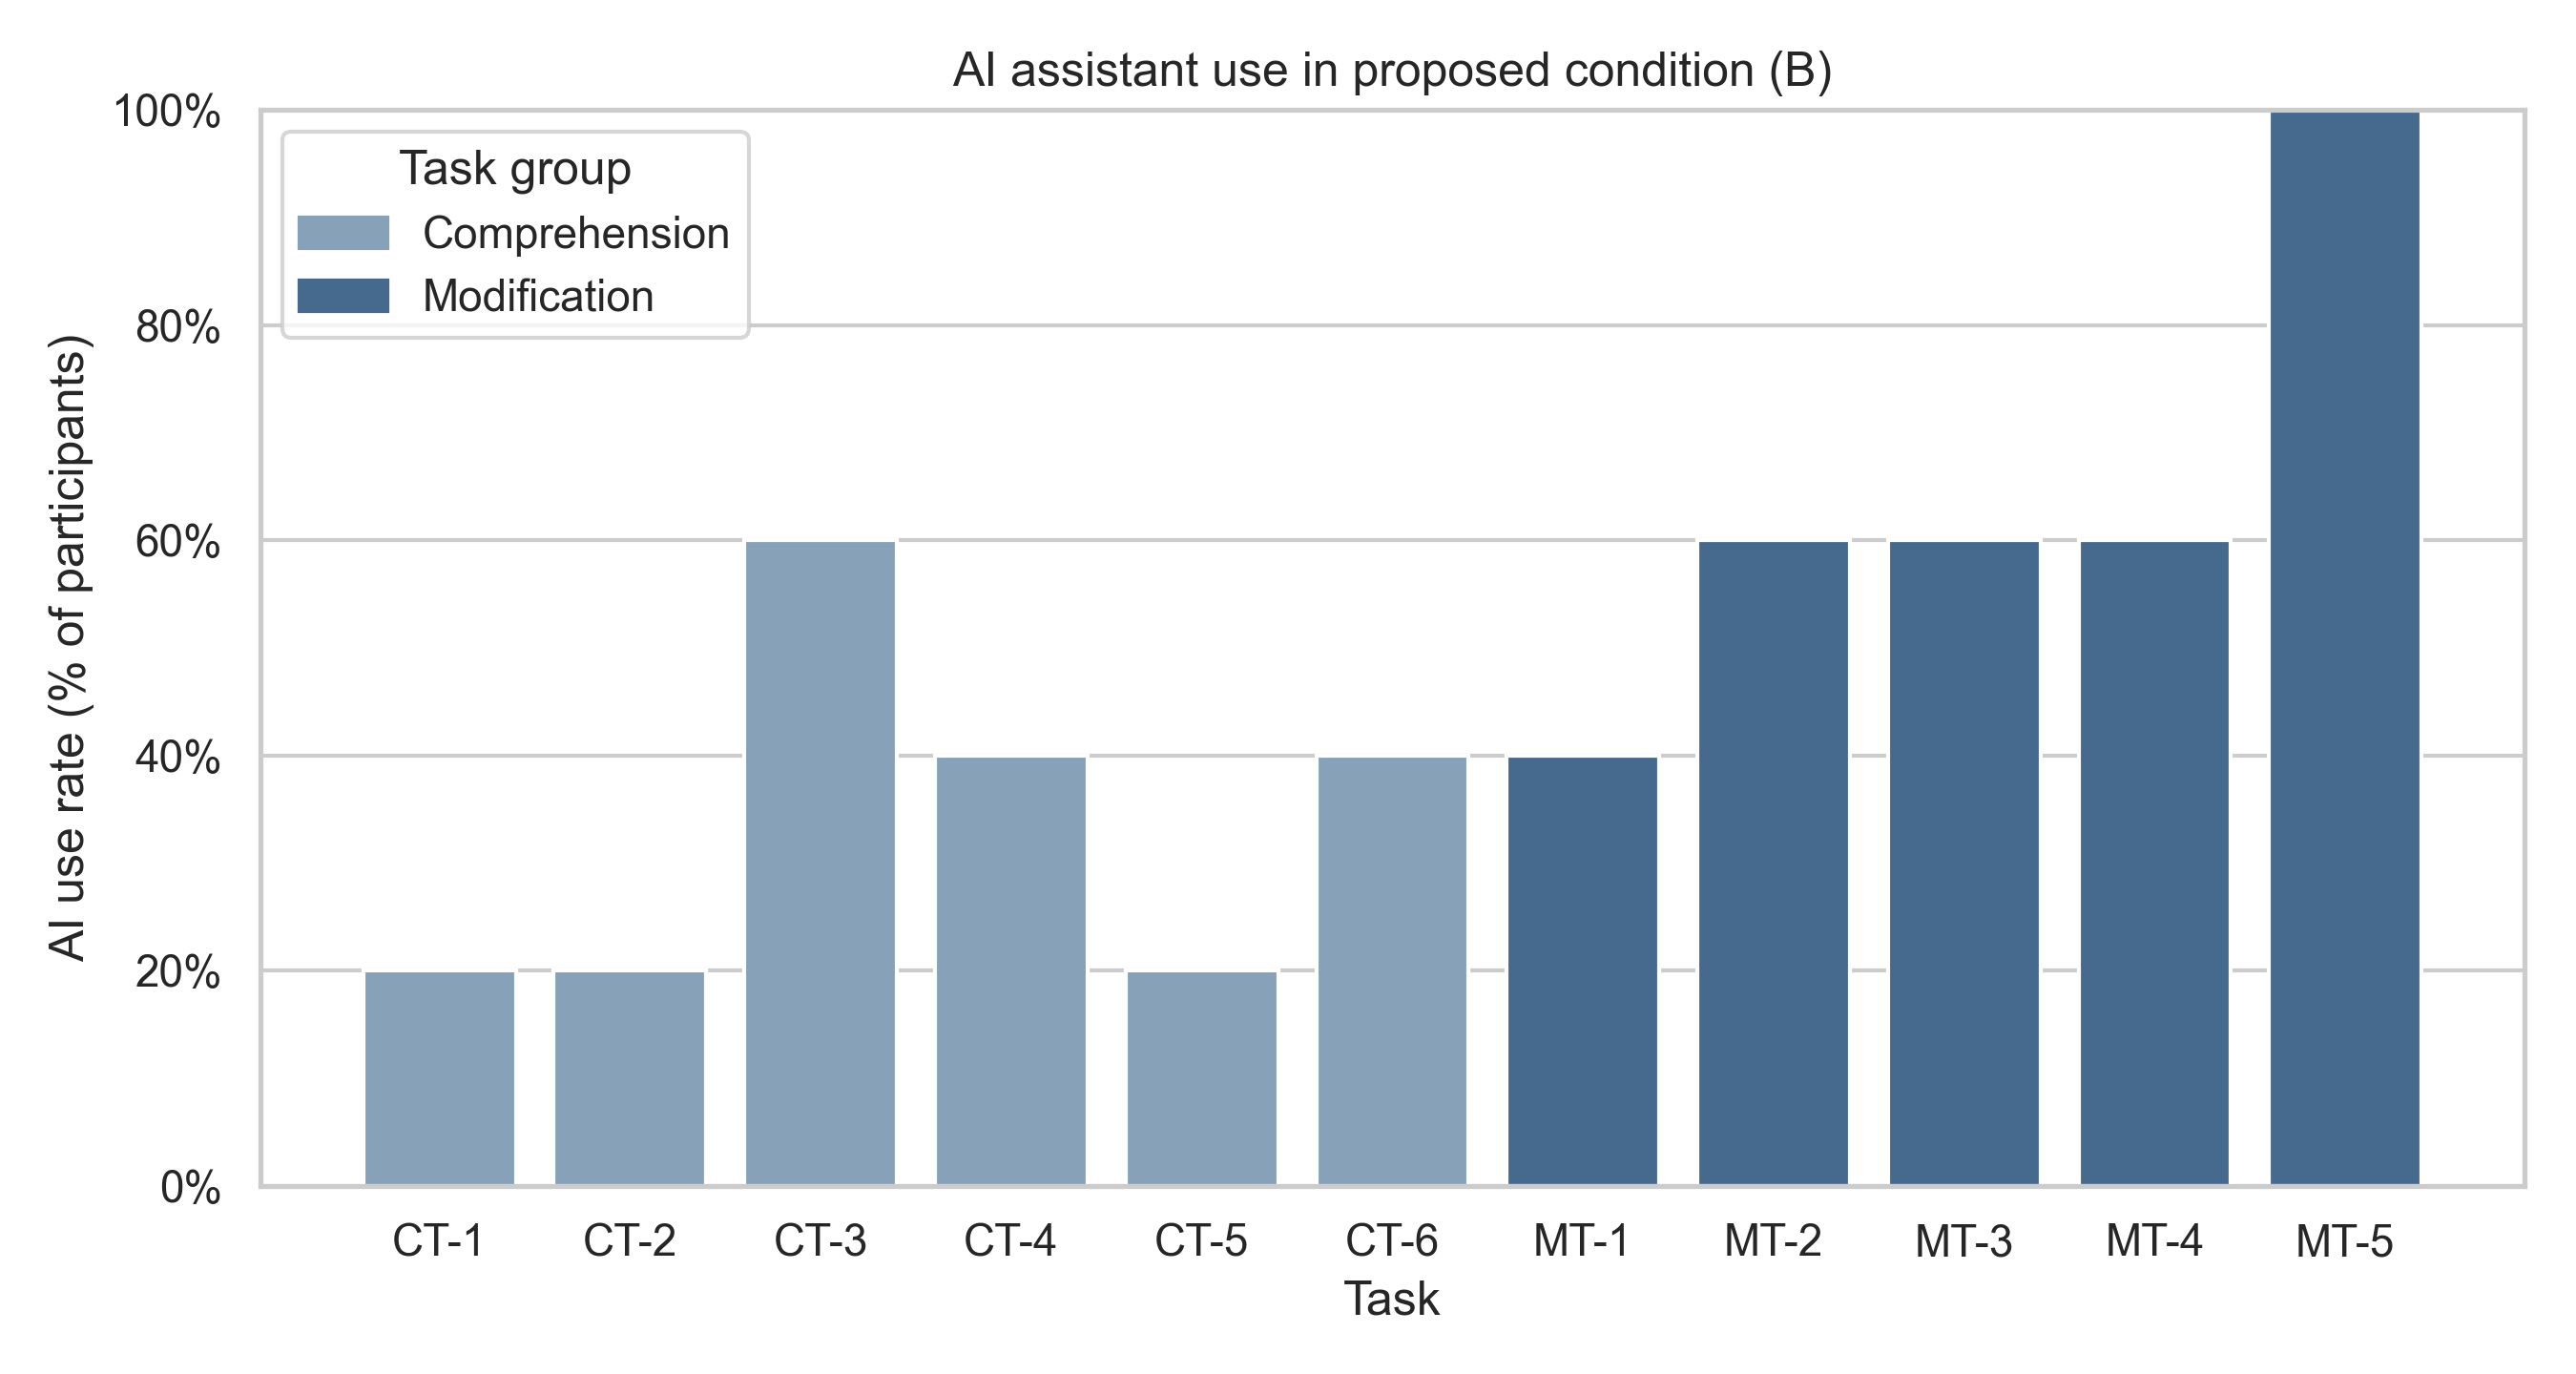
\includegraphics[width=0.82\columnwidth]{media/evaluation/ai_use_rate_by_task.png}
    \caption{AI assistant usage rate by task in condition B (CT-1 -- CT-6 and MT-1 -- MT-5).}
    \label{fig:evaluation:ai-usage}
\end{figure}

Figure \ref{fig:evaluation:assistant-latency-tools} shows the relationship between assistant response time and number of tool calls per assistant request. Across all 43 assistant requests, mean response time was 47.41 s (median 42.56 s). Latency increased with tool-call count. Queries that included program context were slower on average than queries without program context (49.64 s vs. 41.64 s), as reflected by the color split in the plot.

This plot should be interpreted with two caveats. First, the analysis does not explicitly model conversation history or assistant memory carry-over across consecutive sessions. This may partly explain the \textit{no-context} outlier and some of the increasing variability at higher tool-call counts: more retrieved content and prior context can increase effective context-window load. Second, the current context flag is binary and does not distinguish context amount (e.g., a single node snippet vs. an entire program). Thus, the observed latency difference between context and no-context queries may be influenced by the amount of context included in the query, rather than the presence of context alone.

\begin{figure}[H]
    \centering
    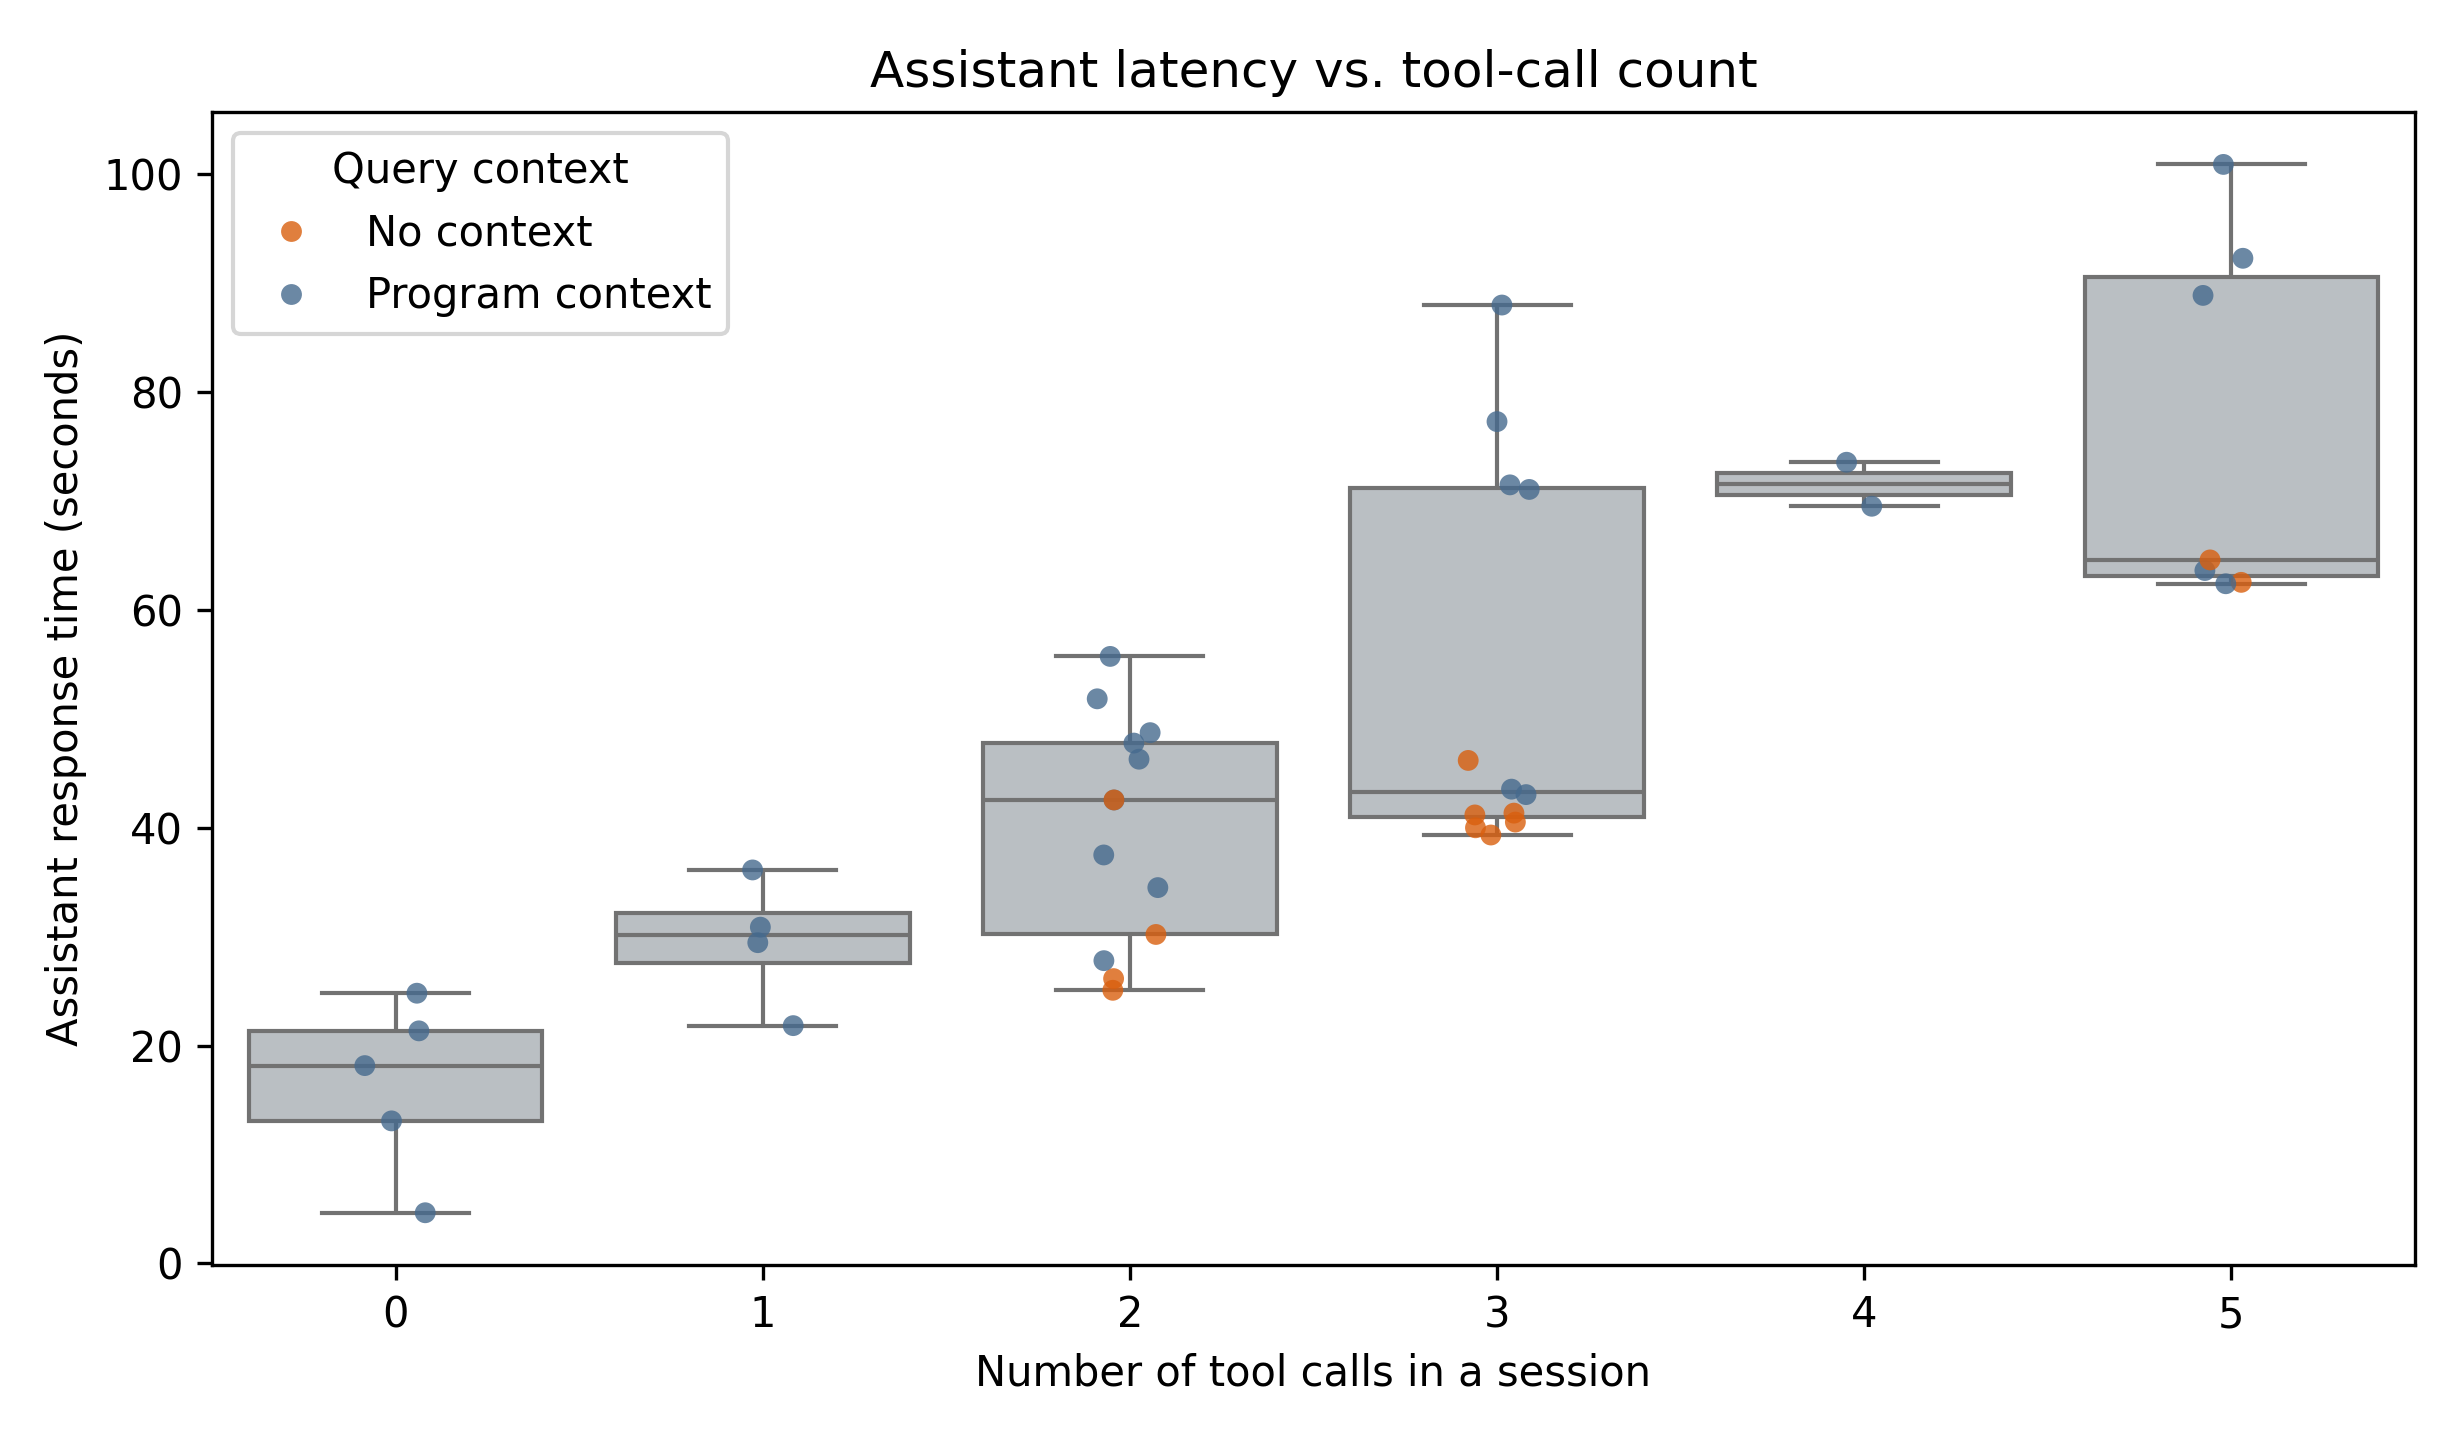
\includegraphics[width=0.82\columnwidth]{media/evaluation/assistant_latency_by_tool_calls.png}
    \caption{AI assistant response time by number of tool calls per assistant request. Points are colored by whether the user included program context in the query.}
    \label{fig:evaluation:assistant-latency-tools}
\end{figure}


\subsection{Post-Study Questionnaire}
Participants provided post-study ratings on various aspects of the system and their experience. The following sections summarize the key findings from these ratings.

\paragraph{Response Comprehension}~\\
The comprehension-response ratings indicate a mixed pattern (Figure \ref{fig:evaluation:post-study-response-comprehension}). Clarity was rated positively by all participants, suggesting that the assistant output was generally readable and understandable. In contrast, ratings for relevance and factual correctness were mostly negative, and quality ratings were split between positive, neutral, and negative responses. Overall, participants could often understand the responses, but frequently questioned whether the content was correct and well aligned with their query.

\begin{figure}[H]
    \centering
    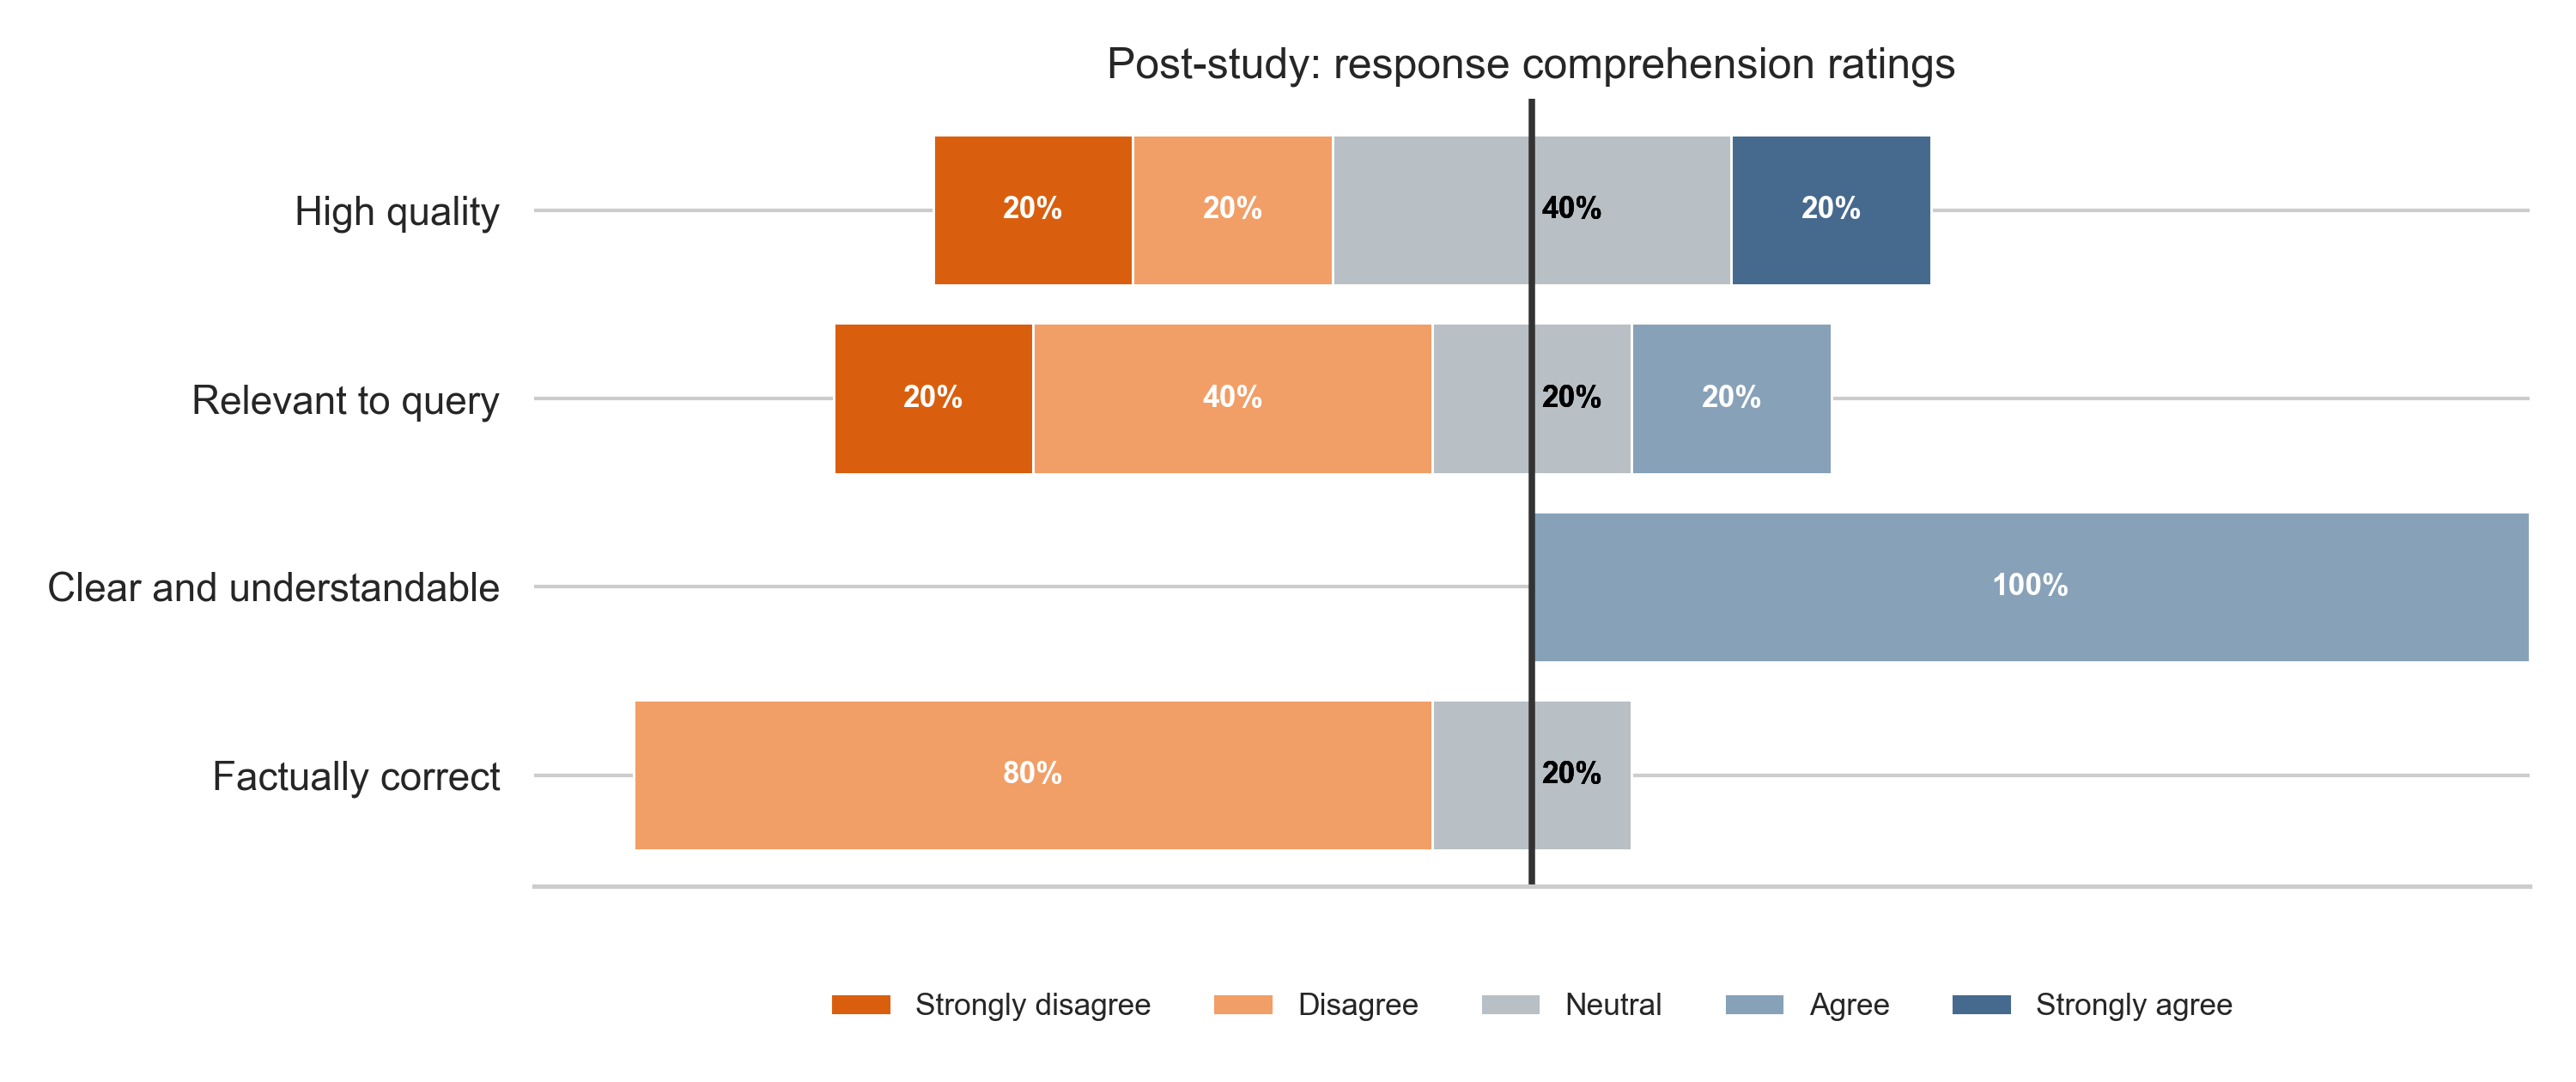
\includegraphics[width=\columnwidth]{media/evaluation/post_study_response_comprehension_diverging.png}
    \caption{Post-study ratings of assistant comprehension responses (quality, relevance, clarity, and factual correctness) shown as a divergent stacked Likert chart.}
    \label{fig:evaluation:post-study-response-comprehension}
\end{figure}

\paragraph{Response Modification}~\\
For modification-response ratings (Figure \ref{fig:evaluation:post-study-response-modification}), clarity again trended more positively than the other dimensions. However, quality and relevance were mainly neutral-to-negative, and factual correctness was rated mostly negatively. This indicates that even when suggestions were understandable, participants often did not consider them sufficiently accurate or directly usable for completing modification tasks.

\begin{figure}[H]
    \centering
    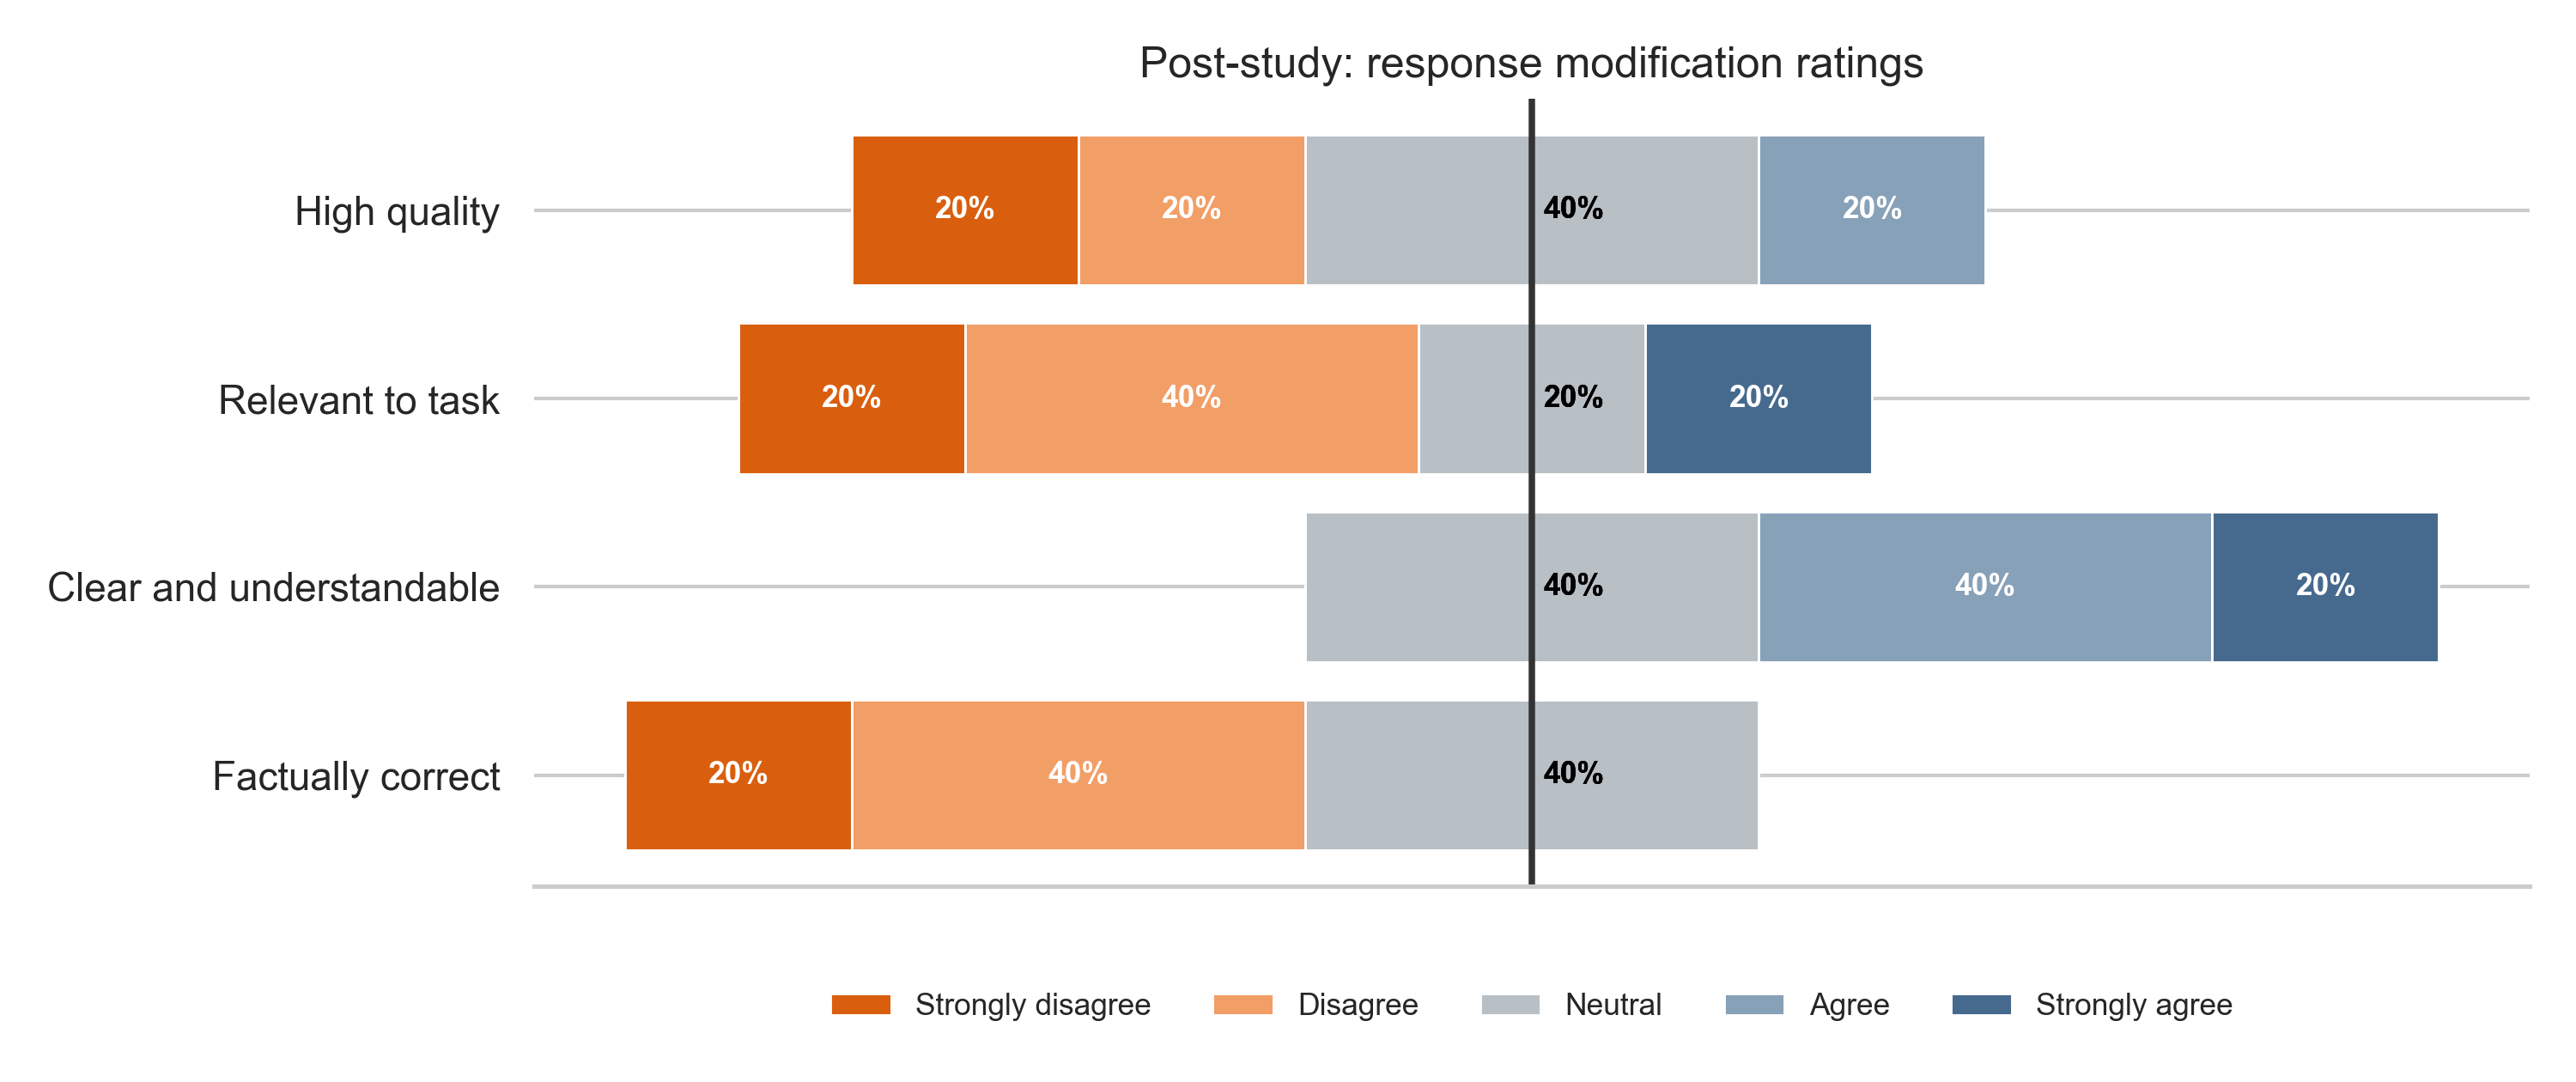
\includegraphics[width=\columnwidth]{media/evaluation/post_study_response_modification_diverging.png}
    \caption{Post-study ratings of assistant modification responses (quality, relevance, clarity, and factual correctness) shown as a divergent stacked Likert chart.}
    \label{fig:evaluation:post-study-response-modification}
\end{figure}

\paragraph{System Usability}~\\
System-usability ratings (Figure \ref{fig:evaluation:post-study-system-usability}) further reflect this tension. Ease of use was polarized, with both clearly positive and clearly negative ratings. Perceived usefulness for robotic program development was predominantly negative, and willingness to use the system in its current form was also mostly negative (with one strong positive outlier). This suggests that while some participants saw potential value in the system, most were not satisfied with its current performance and would not choose to use it for real work without significant improvements.

\begin{figure}[H]
    \centering
    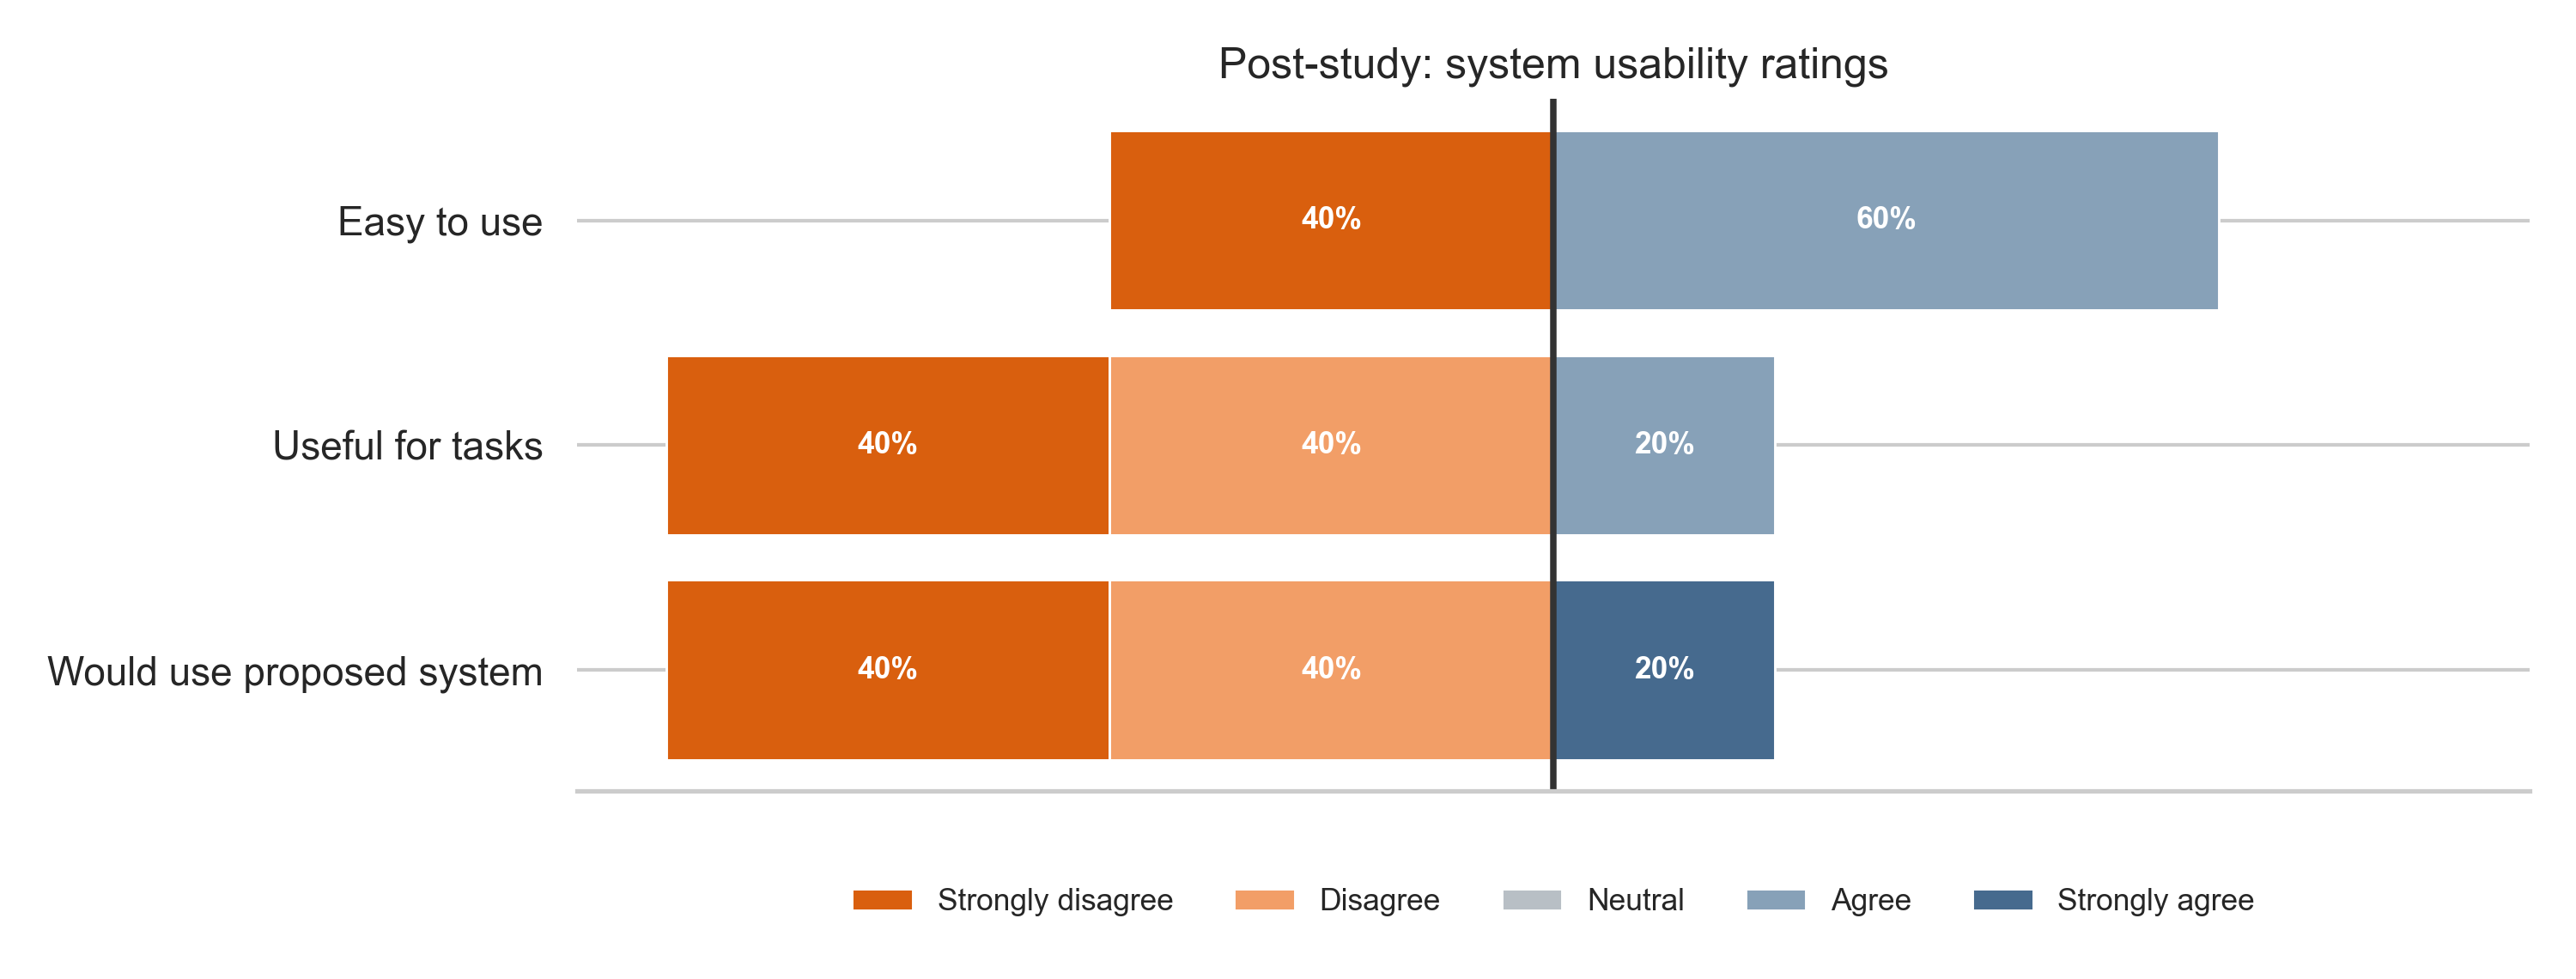
\includegraphics[width=\columnwidth]{media/evaluation/post_study_system_usability_diverging.png}
    \caption{Post-study system-usability ratings (ease of use, perceived usefulness, and willingness to use) shown as a divergent stacked Likert chart.}
    \label{fig:evaluation:post-study-system-usability}
\end{figure}

\subsection{Qualitative Findings}
Open-ended question responses and observations were consistent with the quantitative findings. The open-ended answers show that participants saw clear potential value in the proposed system, but only if it became more reliable and easier to use in practice. In the pre-study responses, participants mainly described AI assistance as useful for speeding up work, helping with drafts, and suggesting possible solutions. In the post-study responses, most participants said they would only use the system after further improvement, and several pointed to the same issues: wrong or irrelevant answers, slow responses, and a lack of direct guidance for changing the program files.

Participants also suggested a number of concrete improvements. The most common requests were for more direct help with the program files, such as line numbers, exact change locations, or code that could be copied into the file. Several participants asked for the system to work more closely with the current open program, to show the active file more clearly, or to add the program as context automatically. Others wanted clearer context handling, the ability to stop requests while the assistant is still working, and a more reliable search experience for discovering programs. Participants were generally not satisfied with the raw \texttt{.urpx} program format and a few suggested either representing programs like UR Studio or as URScript for at better experience.

The observation notes support these comments. Several participants expected the assistant to know the open program automatically, to show line numbers, or to edit the file more directly. Others found it hard to tell whether context had actually been added, or expected the added context to appear under their question rather than only in the assistant response. Some also tried actions that are natural in a file editor but not supported by the proposed system, such as using multiple cursors, and right-clicking or dragging program-tree nodes.

Across participants, the most frequent themes were:
\begin{itemize}
    \item \textbf{Context relevance issues:} Responses were often influenced by earlier prompts or unrelated retrieved context, which made them less useful for the current question. Participants described this as the assistant "remembering" the wrong thing or mixing in unrelated program details.
    \item \textbf{Mismatch between assistance and editing format:} Several responses described actions in the standard UR interface rather than concrete edits in the provided raw \texttt{.urpx} representation.
    \item \textbf{Insufficient actionability:} Participants repeatedly asked for line numbers, exact change locations, or code snippets that could be used directly. This was especially clear in the modification tasks, where the assistant often gave general advice instead of a precise edit.
    \item \textbf{Usability friction:} Participants reported that manual editing in the raw \texttt{.urpx} format is difficult and error-prone. The notes also show several small but important interface problems, such as unclear context attachment, a missing stop button, confusing chat history behavior, lost edits after switching tabs, and difficulty understanding whether context had been added correctly.
    \item \textbf{Performance concerns:} Participants noted that assistant responses were slow and practical barrier to using the system for real work.
\end{itemize}

Overall, the qualitative findings suggest that the general idea of AI assistance is accepted. However, the current implementation lacks quality and features. The main problems of the proposed system are that the assistant does not stay focused on the current query, does not give direct enough help for editing programs, and the program editing interface has several usability issues mentioned above.


\chapter{Discussion}
The evaluation suggests that the overall idea of using an AI assistant to support robotic program comprehension and modification is promising, but the current implementation is not yet a robust solution for practical use. The user study indicates that participants generally understood the value of AI assistance and were willing to try it, but they also encountered substantial friction when the system had to reason over the raw \texttt{.urpx} representation and when the assistant needed to generate concrete editing guidance.

The most positive result is that comprehension correctness remained high in the proposed system. This indicates that the combination of structured program views, retrieval, and assistant explanations can support the basic understanding of robotic programs. However, the lower confidence ratings and the longer completion times show that this support was not frictionless. In other words, the system often helped participants arrive at the correct answer, but it did not make the task feel easier or faster. A large part of the observed time increase appears to come from assistant latency and the interaction overhead of working through chat rather than from the comprehension task itself.

For modification and reuse, the picture is less favorable. The proposed system clearly underperformed the baseline on correctness and completion rate, and the gap was especially visible for tasks that required structural edits. Participants handled parameter updates reasonably well, but tasks that required inserting or restructuring program nodes exposed a mismatch between the system's current interaction model and the actual editing problem. This is consistent with the requirement analysis: the system is expected to support program editing, but the current implementation does so through low-level \texttt{.urpx} editing, which has shown to be a poor fit for many users.

The failure on MT-5 (add wait node) is particularly important. None of the participants completed the wait-node insertion task successfully in the proposed system. This reflects a system limitation. The assistant did not have sufficient knowledge about the exact node structure, and the knowledge base did not contain the required information for this task. In practice, this means the system could not provide the actionable information needed to complete the edit. The result highlights a core dependency of retrieval-augmented systems: if the relevant knowledge is missing, incomplete, or poorly retrieved, the model cannot reliably compensate by generating the right answer on its own.

These findings suggest that the current RAG-style setup works better as a support mechanism for documentation lookup and guided comprehension than as the primary mechanism for code generation and structural modification. For the present domain, the assistant is effectively being used as a one- or few-shot prompt interface over retrieved examples. That is a useful pattern for natural language question answering, but it is a weak foundation for precise program transformation when the target representation is rigid and under-documented. A different editing strategy may therefore be required. Depending on the target user group, a higher-level UI that resembles the teach pendant may be more suitable for novice users, while direct URScript editing may be more appropriate for advanced users. In either case, the edit model should expose domain concepts at a higher level than raw \texttt{.urpx} nodes.

The two conditions, the baseline and the proposed system, differed on multiple dimensions simultaneously, so it is not possible to attribute observed differences in correctness or time to the assistant alone. The baseline condition offered a visual, teach-pendant-like interface, while the proposed system combined JSON editing with chat-based assistance. The observed differences therefore reflect the combined workflow rather than isolating the assistant's contribution. This is an important caveat when interpreting the results: the assistant may have provided useful information, but the overall workflow was more cumbersome than the baseline, which likely contributed to lower confidence and longer completion times. On the other hand, the assistant may have provided misleading information in some cases, which could have contributed to incorrect answers or lower user confidence in their own solutions. The study design does not allow us to disentangle these effects, so the results should be interpreted as reflecting the overall user experience of the proposed system rather than the assistant's performance in isolation.

The results further indicate that response quality depends strongly on the retrieved context. When the retrieval pipeline surfaced relevant material, the assistant was often understandable and occasionally useful. When the retrieved material was sparse or tangential, the assistant produced weaker answers. This makes data coverage and retrieval quality central design concerns. More data, better chunking, and improved similarity search are likely to have a direct effect on usefulness.

At the same time, the current approach raises the question of whether fine-tuning would be a better fit than pure RAG for code-oriented tasks. Fine-tuning a general coding model on a domain-specific URScript or robot-program dataset would require substantial upfront effort, but it could improve structural editing, domain terminology, and output consistency. RAG would still be valuable for domain documentation and project-specific retrieval, so the two approaches are not mutually exclusive. A hybrid design seems most plausible: use retrieval for factual and project-specific context, and use a specialized or fine-tuned model for code generation and modification.

Finally, the response-time results are a practical warning. Even if the outputs are useful, a slow assistant will be difficult to adopt in everyday programming workflows. Some of the latency stems from retrieval and model inference, but part of the problem is also the user experience: participants have to wait for the full answer before they can continue. This suggests that both system optimization and interface changes are needed. Streaming responses, exposing progress indicators, and reducing orchestration overhead would improve perceived responsiveness even before the underlying model stack is fully optimized.

\section{Implications for the Requirements}
The evaluation provides partial support for the requirements defined earlier in the thesis, but also shows where the requirements remain unmet in practice.

For the functional requirements, the strongest support is for requirements related to comprehension and question answering. The study results indicate that FR5 and FR7 are partially satisfied, since the assistant could often answer natural-language questions and participants achieved near-perfect comprehension correctness. FR6 also appears largely satisfied because users generally rated response clarity positively. FR10 is only partially satisfied: in several cases participants perceived low factual correctness or relevance, indicating that uncertainty handling and reliability were not consistently strong.

Requirements related to modification and direct editing support are less well satisfied. FR8 is not sufficiently satisfied in its current form, as modification correctness dropped substantially in the proposed condition. FR4 is also only partially satisfied from a usability perspective: although an editor exists, editing raw \texttt{.urpx} structures introduced substantial friction for structural changes. Requirements tied to overall repository workflow, namely FR1-FR3, were not the primary focus of the controlled tasks, so the current evaluation provides only limited evidence for their practical effectiveness under realistic usage.

FR9 is partially supported. The system retains session context, but qualitative findings indicate that context was not always perceived as relevant by users and may sometimes have introduced irrelevant carry-over. This suggests that conversational memory exists technically, but context selection and grounding need improvement.

The non-functional requirements are also mixed. NFR1 (response within 10 seconds) is not met in the observed user workflow, where assistant response times were substantially higher. NFR2 (modifiability through isolation of LLM functionality) is architecturally supported by the system design. NFR3 (observability) is well-supported through detailed logging, and NFR4 (traceability) is supported as retrieved references are exposed.

For usability-oriented requirements, NFR5 is the most supported because response clarity was generally rated positively. In contrast, NFR6 and NFR7 are not supported by the present results, since perceived usefulness for comprehension and especially modification was limited. NFR8 and NFR9 are also not sufficiently satisfied, as post-study ratings frequently questioned response relevance and factual correctness.

\section{Threats to Validity}
Several limitations affect the strength of the results. The sample size was only five participants, which is too small to support broad generalization. The study also evaluated the system as a whole rather than isolating the assistant from the editor and retrieval pipeline, so the measured differences reflect the combined workflow.

The task set was narrow. The modification tasks focused on relatively basic parameter changes and node insertions, so the results do not reveal how the system would perform on more complex programming tasks. In addition, the tasks were performed in a fixed order within each condition, which may have introduced order effects even though the overall condition order was counterbalanced.

The timing data should also be interpreted with caution because task durations were measured manually with a stopwatch. This introduces measurement noise and makes small time differences difficult to interpret precisely.

The evaluation did not directly score assistant response correctness. A participant could use the assistant, receive an unhelpful answer, and still complete the task independently. In that case, the study records both assistant use and task success, but it does not distinguish how much the assistant actually contributed to the outcome.


\section{Future Work} \label{sec:discussion:future-work}
Future work should focus on improving the assistant along four dimensions: data coverage, retrieval quality, interaction design, and evaluation methodology.

\subsection{Data and Knowledge Base}
The most direct improvement is to expand the knowledge base. More robot programs, more documentation, and more examples of domain-specific structures would make retrieval more reliable. In addition to official Universal Robots documentation, useful sources would include partner material, customer examples, support forums, and community discussions such as Discord or other Q\&A channels. The assistant would likely benefit from more question-answer pairs, more annotated program examples, and better coverage of uncommon node types and editing patterns.

\subsection{Retrieval and Prompting}
Better retrieval can improve response quality. Better chunking strategies, hybrid similarity search, and improved query rewriting may all improve the relevance of retrieved context. Prompt engineering is another low-cost opportunity: better system prompts, clearer task framing, and more explicit instructions for uncertainty handling could improve response quality without changing the overall architecture.

In addition, the orchestration logic should be improved, so the assistant makes better decisions about when to retrieve, which source type to query, and how many tool steps are actually needed before synthesis. The current behavior suggests that unnecessary or weakly targeted tool calls can increase latency and sometimes reduce response quality by introducing noisy context.

Memory management is also an important improvement area. Future versions should use stronger context-selection policies, so prior conversation history does not over-pollute new responses with stale or irrelevant details.

At the same time, a pure RAG setup may not be the best long-term solution for code generation and program modification. A hybrid approach may be more promising: use retrieval for documentation and project-specific facts, and use a specialized model for code-oriented reasoning. A fine-tuned model trained on URScript or a similar domain-specific corpus could be more reliable for edits, especially when the output must follow strict structural constraints. Such a model would require a suitable dataset and more training effort, but it could reduce the dependence on fragile few-shot prompting.

\subsection{Editing Workflow and User Interface}
The editing workflow should be reconsidered. Raw \texttt{.urpx} editing is a poor interaction model for many users because the representation is too low-level for novice users and too brittle for structural edits. Future versions should either provide a higher-level interface inspired by the teach pendant or support direct URScript editing for advanced users. Which option is preferable depends on the intended user group, but both would likely be more usable than editing the raw program file.

More agentic behavior would elevate the assistant's capabilities: the assistant should be able to inspect the current program, propose edits, validate them, and ideally help execute or simulate the programs.

An integration with a language server protocol could also be useful if the editing workflow is based on text or structured program files. A language server could provide syntax awareness, hover information, references, diagnostics, and code actions. That would make the assistant less dependent on ad hoc prompting and would ground its suggestions in the structure of the actual program format.

\subsection{Performance and Responsiveness}
Improving response time is important for usability. One option is to use a smaller and more specialized orchestration model, reserving larger models only for tasks that actually need them. Another option is to stream more intermediate progress and the final answer, so users do not have to wait while retrieval and generation are running. If the system displays intermediate progress, users may better tolerate latency even when the underlying response time remains nontrivial.

Another direction of improvement is to move away from a local-only model setup. While local deployment is useful for early prototyping, future versions should evaluate hybrid or cloud-hosted model serving for demanding tasks. This could provide access to stronger models, faster inference, and more stable response quality. A practical approach is a hybrid routing strategy in which routine requests are handled locally, while complex requests are escalated to hosted models when higher capability is needed.

\subsection{Evaluation}
Future evaluations should use a larger and more diverse participant sample to improve generalizability. Task timing should be automated rather than measured manually. The task order should also be counterbalanced within each condition so that task-specific order effects are reduced.

The evaluation should additionally measure assistant response correctness directly, not only final task correctness. This would make it possible to separate cases where the assistant was helpful from cases where the participant succeeded despite the assistant. Future studies should also include a broader task set, including more complex edits and more realistic programming scenarios, so that the limits of the system are better understood.

\chapter{Conclusion}
This thesis investigated how large language models can be used to support natural language-based comprehension and reprogrammability of robotic programs. The work contributed an architecture and implementation of an LLM-assisted system that combines retrieval-augmented generation, program/document indexing, and a user interface for exploration and modification of Universal Robots robotic programs.

The evaluation shows a mixed but informative outcome. For comprehension, the proposed system preserved near-perfect correctness (RQ1), indicating that retrieval-supported assistant responses and structured program views can help users identify key program properties even when working with low-level representations. However, comprehension time increased (RQ2), and confidence was lower than in the baseline condition. A significant part of the time increase is linked to assistant latency and interaction overhead rather than task complexity alone.

For modification and reuse, the findings are less favorable. The proposed system reduced modification correctness and increased completion time (RQ3 and RQ4), especially for tasks requiring structural edits such as node insertion. Participants were more successful on straightforward parameter updates than on transformations requiring deeper structural understanding of raw \texttt{.urpx} data. This indicates that the current workflow and representation are not yet a suitable foundation for reliable editing support in practical settings.

Together, the results answer the main research question as follows: LLMs can support natural language-based robotic program comprehension, but robust support for reprogrammability requires stronger grounding, better domain coverage, and a better editing abstraction than the one implemented in this thesis.

Beyond performance comparisons, the thesis contributes empirical insight into design pitfalls for robotics-oriented LLM systems. In this domain, response quality is strongly dependent on knowledge-base coverage and retrieval quality, and usability is highly sensitive to latency. The results also highlight that system-level workflow design matters as much as model capability: a chat assistant layered on top of a low-level program representation can help users reason about code, but it does not automatically make complex edits easier.

In conclusion, this thesis provides a practical baseline for continued work in LLM-assisted robotic programming. The findings suggest that future systems should combine improved retrieval and data quality with either higher-level editing abstractions or specialized model support for program transformations. With these improvements, the approach has clear potential to reduce barriers to robot program comprehension, modification, and reuse.


\newpage
%TC:ignore
\bibliographystyle{unsrturl}
\bibliography{references}
%TC:endignore

\newpage
%TC:ignore
\begin{appendices}
    \chapter{Digital Appendix Overview} \label{appendix:digital-appendix-overview}
This appendix provides an overview of the digital appendix.

\begin{itemize}
    \item The \path{/masters-thesis/app} directory contains the application code.
    \item The \path{/masters-thesis/data} directory contains the data (robot programs, program metadata, and documentation) used in the application.
    \item The \path{/masters-thesis/evaluation} directory contains the evaluation robot programs, analysis scripts, and results.
\end{itemize}

    \chapter{Implementation Prompts} \label{appendix:implementation-prompts}

\section{Agent Prompt}

\begin{minted}[fontsize=\footnotesize, breaklines]{python}
def get_agentic_routing_system_prompt() -> str:
    """System prompt for the agentic retrieval stage.
    
    The agent intelligently calls tools to gather relevant information, then evaluates
    whether the retrieved context sufficiently answers the query before deciding to stop.
    This enables adaptive, context-aware retrieval.
    """

    return f"""You are an intelligent retrieval assistant for a robot documentation and program retrieval system.

Your job is to ADAPTIVELY gather relevant information by:
1. Calling tools to retrieve context
2. Evaluating if the retrieved content answers the query
3. Deciding whether to STOP or call more tools
4. Do NOT synthesize the final answer - a separate system will do that

Available tools:
1. search_robot_programs(query, limit): search for robot program metadata and summaries.
2. search_robot_code(query, limit): search for extracted robot program code snippets.
3. search_documentation(query, limit): search for technical documentation chunks.

## Core Workflow (ADAPTIVE CONTEXT-AWARE RETRIEVAL)
**Step 1: Retrieve**
- Call 0-2 tools based on your initial understanding of the query
- Each tool call should have a specific purpose (e.g., "search for program examples" or "find configuration docs")

**Step 2: Evaluate Retrieved Context**
After each tool call, examine the results:
- **Relevance**: Are the results addressing the query's core question?
- **Sufficiency**: Do you have enough information to answer the query?
- **Gaps**: What information is still missing?

**Step 3: Decide (CRITICAL - THIS IS THE ADAPTIVE PART)**
Based on your evaluation, choose:

**STOP if**:
  - You retrieved 2+ relevant documents that directly address the query
  - The results contain concrete examples, code, or explanations matching the query
  - For queries about specific programs: you found the program or similar examples
  - For technical queries: you found documentation explaining the concept
  - For modification queries: you found code patterns or guidance relevant to the modification

**CONTINUE if**:
  - You got 0 results (try a different tool or refined query)
  - Results seem off-topic or irrelevant to the actual question
  - Results are too sparse (1 doc for a query needing examples)
  - You haven't yet tried the most relevant tool for this query type
  - For example: retrieved docs are about unrelated topics, no code examples when examples are needed

## Concrete Decision Examples
**Scenario A: "Show me pick-and-place programs"**
1. Call search_robot_programs("pick-and-place", 2)
2. Results: returns 2 programs with "pick-and-place" in metadata
3. Evaluate: "These are directly relevant pick-and-place programs - Sufficient"
4. **DECISION: STOP** - You have what you need

**Scenario B: "How do I configure the gripper payload?"**
1. Call search_documentation("gripper payload configuration", 2)
2. Results: returns 1 technical doc with payload config details + 1 unrelated doc
3. Evaluate: "Got 1 highly relevant doc explaining payload config - Sufficient"
4. **DECISION: STOP** - You have configuration guidance

**Scenario C: "Modify this program to use a different motion primitive"**
1. Call search_robot_code("motion primitive", 2)
2. Results: returns 0 relevant results (or only generic code)
3. Evaluate: "No code examples for motion primitives - Insufficient"
4. **DECISION: CONTINUE** → Call search_documentation("motion primitive types", 2)
5. Results: returns documentation on motion primitives
6. Evaluate: "Now have both code context and documentation - Sufficient"
7. **DECISION: STOP** - Combined retrieval answered the query

**Scenario D: "What's the capital of France?"**
1. Analyze query: This is general knowledge, not about robots
2. Evaluate: No retrieval needed
3. **DECISION: STOP immediately** (call no tools) - General knowledge doesn't need retrieval

## Important Rules
- Maximum 5 documents per tool call
- Call at most 3-4 tools total across the retrieval session
- After 2 unsuccessful tool calls (no relevant results), check if retrieval is actually needed
- Always prioritize the most specific tool for the query (don't search all 3 databases if 1 is sufficient)
- Trust your evaluation - if you have good answers, STOP early. Don't over-retrieve.

## Your Evaluation Criteria
When examining retrieved results, ask yourself:
1. "Do these results directly address the core question?"
2. "If the user received only these results, would they be satisfied?"
3. "Are there obvious gaps or missing information I should fill?"
4. "Have I tried all relevant tools, or should I try another approach?"

Then decide: **STOP or CONTINUE**."""
\end{minted}
\captionof{listing}{Agent prompt.}
\label{listing:appendix:agent_prompt}


\newpage
\section{Synthesis Prompt}

\begin{minted}[fontsize=\footnotesize, breaklines]{python} 
def get_synthesis_prompt_template() -> ChatPromptTemplate:
  """
  Chat prompt template for response synthesis from retrieved documents.
  """
  system_template = """You are a helpful assistant for UR robot programming and technical questions.

Your task is to answer the user's question based on the current query and the provided context.

## Guidelines:
1. **Answer the current query first**: Treat the user's latest message as the primary signal
2. **Use provided context**: Use retrieved documents and supplied program context to support the answer
3. **No inline citations list**: Do not append a references/sources list in the answer body
4. **Multi-part answers**: If discussing programs, organize information clearly with examples
5. **Acknowledge limits**: If the context doesn't fully answer the question, say so
6. **Conversation history**: Treat conversation history as secondary context for continuity, not as the primary source of truth
7. **Ambiguity handling**: If the current query is unclear or vague, ask for clarification rather than assuming it refers to previous topics
8. **Format**: Respond in clean Markdown only

If retrieval was incomplete, do not fail the answer. Give the best partial answer you can from the retrieved context, and explicitly say what is still unknown or uncertain. If there is not enough evidence to answer safely, say that you do not know.

## Markdown Output Rules (strict):
1. Use short headings with `##` and `###`.
2. Always put headings on their own line.
3. Leave one blank line after each heading.
4. Use bullet lists (`-`) or numbered lists (`1.`) for structured points.
5. Keep paragraphs short (1-3 sentences).
6. Do not add a `Sources`, `References`, or `Citations` section.
7. If information is uncertain or missing, add a `## Limitations` section.
8. Do not output JSON.
9. Do not put markdown markers and text on the same line incorrectly (for example avoid `### Heading text continues without spacing issues`).

Note: Source provenance is shown separately by the UI metadata dropdown. Keep the answer focused on content only."""

  human_template = """## Retrieval Status
{retrieval_status}

## Current User Query:
{query}

## Primary Context (Retrieved Documents and Provided Program Context):
{context}

## Secondary Context (Conversation History - Only use this for continuity, not as the main source of truth):
{history}

Provide a helpful, detailed answer based on the current query and primary context above using the Markdown rules."""

  return ChatPromptTemplate.from_messages(
    [
      ("system", system_template),
      ("human", human_template),
    ]
  )
\end{minted}
\captionof{listing}{Synthesis prompt.}
\label{listing:appendix:synthesis_prompt}
    \chapter{Evaluation Protocol} \label{appendix:evaluation-protocol}

\section{Introduction}
The evaluation will focus on four research questions (RQ1, RQ2, RQ3, RQ4) that assess the correctness of comprehension, time required for completion of comprehension tasks, and the correctness and time required for modification and reuse of robot programs. The study design for evaluating the proposed system is structured to systematically assess its impact on the comprehension and modification of robotic programs. The evaluation will be conducted through a controlled user study, where participants will be tasked with comprehending and modifying robotic programs using both the proposed system and a traditional baseline approach.

\begin{adjustwidth}{\indentWidthTwenty}{\indentWidthTwenty}
    \textit{\textbf{RQ1:} How does the proposed system influence the correctness of comprehension of robotic programs?}
\end{adjustwidth}
\begin{adjustwidth}{\indentWidthTwenty}{\indentWidthTwenty}
    \textit{\textbf{RQ2:} How does the proposed system influence the time required for comprehension of robotic programs?}
\end{adjustwidth}
\begin{adjustwidth}{\indentWidthTwenty}{\indentWidthTwenty}
    \textit{\textbf{RQ3:} How does the proposed system influence the correctness of modification and reuse of robot programs?}
\end{adjustwidth}
\begin{adjustwidth}{\indentWidthTwenty}{\indentWidthTwenty}
    \textit{\textbf{RQ4:} How does the proposed system influence the time required in the modification and reuse of robot programs?}
\end{adjustwidth}

For the baseline approach, UR Studio will be used. UR Studio is a browser based simulation tool for UR robots created by Universal Robots. It provides a visual programming interface, similar to programming directly on the teach pendant, for creating and simulating robotic programs.

\section{Study Design}
The study employs a within-subjects design, where each participant will experience both conditions (proposed system and baseline) in a counterbalanced order to mitigate potential learning effects.

To further mitigate learning effects, the evaluation consists of two phases for each condition: an exploration phase and a task phase.
\begin{itemize}
    \item \textbf{Exploration Phase:} In the exploration phase, participants will familiarize themselves with the system. This phase will involve guided walkthroughs and practice tasks to ensure that participants have a sufficient understanding of the condition before proceeding to the task phase.
    \item \textbf{Task Phase:} In the task phase, participants will be given specific comprehension and modification tasks to complete using the assigned condition. The tasks will be designed to assess the research questions, with a focus on measuring correctness and time taken for both comprehension and modification activities.
\end{itemize}


\subsection{Pre-Study Survey}
Before the study begins, participants will complete a pre-study survey to collect their perceived experience level with robotic programming and familiarity/use of AI-assistants. This information will be used to analyze potential correlations between participant characteristics and their performance in the study.


\subsection{Task Design}
The tasks will be designed to reflect realistic scenarios that users may encounter when working with robotic programs. They will be structured to evaluate both comprehension and modification aspects, with a focus on assessing the correctness of understanding and the efficiency of modifications.

Two types of tasks will be included:
\begin{itemize}
    \item \textbf{Comprehension Tasks:} Participants will be asked to read and understand robotic programs, answer questions about their functionality, and identify key components and logic. The tasks will be designed to assess the depth of comprehension, the ability to extract relevant information from the programs and the time taken to complete the comprehension tasks.
    \item \textbf{Modification Tasks:} Participants will be given specific requirements for modifying existing robotic programs. They will be tasked with making changes to the code to meet new specifications or adapt it to different contexts. The tasks will evaluate both the correctness of the modifications and the time taken to complete them.
\end{itemize}

Correctness will be assessed based on predefined criteria for each task. For the comprehension tasks, correctness will be measured based on whether participants select the correct answer for each multiple-choice question. Comprehension performance will be quantified using the number of correctly answered questions and the time taken to complete the tasks. For the modification tasks, correctness will be determined by whether the implemented modifications satisfy the specified task requirements without introducing functional errors. The modified programs will be evaluated against predefined expected outcomes, including successful execution of the intended behavior and preservation of existing functionality where applicable. Partial correctness will be considered for modifications that satisfy some, but not all, of the required changes.

To further mitigate learning effects, the robot programs and the modification tasks will be designed to be sufficiently distinct across conditions, ensuring that participants cannot simply apply knowledge gained from one condition to the other.

Combining the counterbalanced design with distinct task sets for each condition:
\begin{table}[H]
    \centering
    \begin{tabular}{p{0.1\textwidth} p{0.32\textwidth} p{0.32\textwidth}}
        \hline
                & \textbf{Condition 1}           & \textbf{Condition 2}           \\
        \hline
        Group 1 & Baseline + Task set \#1        & Proposed System + Task set \#2 \\
        Group 2 & Proposed System + Task set \#1 & Baseline + Task set \#2        \\
        \hline
    \end{tabular}
    \caption{Counterbalanced and learning mitigation design.}
\end{table}

\subsection{Metrics}
The evaluation will utilize a combination of quantitative and qualitative metrics to assess the impact of the proposed system on comprehension and modification of robotic programs.

Quantitative metrics will include:
\begin{itemize}
    \item \textbf{Correctness of Comprehension:} This will be measured by the number of correctly answered multiple-choice comprehension questions.
    \item \textbf{Time for Comprehension:} The time taken by participants to complete the comprehension tasks will be recorded and analyzed.
    \item \textbf{Correctness of Modifications:} The accuracy of modifications made by participants will be evaluated against predefined criteria based on the task requirements.
    \item \textbf{Time for Modifications:} The time taken to complete modification tasks will be recorded and analyzed.
    \item \textbf{Confidence Levels:} After each task completion, participants will be asked to rate their confidence in their comprehension and modifications on a Likert scale (1 to 5), providing insight into their subjective experience with the system.
\end{itemize}

Qualitative metrics will include:
\begin{itemize}
    \item \textbf{System-wide User Feedback:} Participants will be asked to provide feedback on their experience using the proposed system, including perceived usability, usefulness, and any challenges encountered during the tasks.
    \item \textbf{LLM-assisted User Feedback:} Participants will be asked to provide specific feedback on the proposed system's LLM-assisted features, such as the quality of generated responses and the relevance of suggestions for modifications.
    \item \textbf{Observational Data:} The evaluation will also include observational data collected during the study, such as participant behavior, interactions with the system, use of AI-assisted features, and any difficulties faced during comprehension and modification tasks.
\end{itemize}


\subsection{Participants}
The study will recruit potential users of the proposed system, including robotics engineers and programmers who have experience working with robotic systems. Participants will be sourced from relevant industry professionals and academic institutions.


\subsection{Questions}
\subsubsection{Pre Study Questions}
\begin{itemize}
    \item How would you rate your experience level with robotic programming? (Likert scale 1-5)
    \item How often do you use AI assistants for software development? (Likert scale 1-5)
    \item I would use an AI assistant for developing robot programs? Explain why or why not? (Likert scale 1-5 + open-ended response)
\end{itemize}

\subsubsection{Task Questions}
Comprehension Tasks:
\begin{itemize}
    \item Identify the key actions used in the robotic program. (Multiple choice)
    \item Choose the correct sequence of actions in the order performed by the robot in the program. (Multiple choice)
    \item Choose the correct sequence of waypoints in the order they are reached by the robot in the program. (Multiple choice)
    \item Does the program use any URCap? (Multiple choice)
    \item Which gripper does the program use? (Multiple choice)
    \item Which of the following overall applications best match the program. (Multiple choice)
    \item I feel confident in my program comprehension. (Likert scale 1-5)
\end{itemize}

Modification Tasks:
\begin{table}[H]
    \centering
    \begin{tabular}{p{0.01\textwidth} p{0.44\textwidth} p{0.44\textwidth}}
        \hline
           & \textbf{Task set \#1}                                      & \textbf{Task set \#2}                                      \\
        \hline
        1. & Change the speed of the first move action.                 & Change the speed of the last move action.                  \\
        2. & Change the movement type of the last move action.          & Change the movement type of the first move action.         \\
        3. & Switch the waypoints of the second and third move actions. & Switch the waypoints of the fourth and fifth move actions. \\
        4. & Enable blend movement of the second move action.           & Enable blend movement of the third move action.            \\
        5. & Add a wait action after the last move action.              & Add a wait action after the first move action.             \\
        \hline
    \end{tabular}
    \caption{Modification task sets.}
\end{table}

\subsubsection{Post Study Questions}
\begin{itemize}
    \item The proposed system was easy to use. (Likert scale 1-5)
    \item The proposed system was useful for robotic programming tasks. (Likert scale 1-5)

    \item LLM-generated comprehension responses:
          \begin{itemize}
              \item The LLM-generated comprehension responses were of high quality. (Likert scale 1-5)
              \item The LLM-generated comprehension responses were relevant to my query. (Likert scale 1-5)
              \item The LLM-generated comprehension responses were clear and understandable. (Likert scale 1-5)
              \item The LLM-generated comprehension responses were factually correct. (Likert scale 1-5)
          \end{itemize}

    \item LLM-generated modification suggestions:
          \begin{itemize}
              \item The LLM-generated modification suggestions were of high quality. (Likert scale 1-5)
              \item The LLM-generated modification suggestions were relevant to the modification task. (Likert scale 1-5)
              \item The LLM-generated modification suggestions were clear and understandable. (Likert scale 1-5)
              \item The LLM-generated modification suggestions were factually correct. (Likert scale 1-5)
          \end{itemize}

    \item I felt confident in my program comprehension when using the proposed system. (Likert scale 1-5)
    \item I felt confident in my program modifications when using the proposed system. (Likert scale 1-5)
    \item I felt confident in my program comprehension when using the baseline approach. (Likert scale 1-5)
    \item I felt confident in my program modifications when using the baseline approach. (Likert scale 1-5)

    \item What challenges did you encounter while using the proposed system during the tasks? (Open-ended response)
    \item Do you have any suggestions for improving the proposed system? (Open-ended response)
    \item I would use the proposed system in my robotic programming work. Explain why or why not. (Likert scale 1-5 + open-ended response)
\end{itemize}
    \chapter{Evaluation Data} \label{appendix:evaluation-data}

\newcommand{\CsvVerbatimInput}[1]{%
    \VerbatimInput[
        fontsize=\tiny,
        breaklines=true,
        breakafter={,},
        % breaksymbolleft={},
        breaksymbolright={},
        breakaftersymbolpre={},
        breakaftersymbolpost={}
    ]{#1}%
}

This appendix provides the raw evaluation results used in Chapter \ref{chapter:evaluation}. The same result and log files are also available in the digital appendix (see Appendix \ref{appendix:digital-appendix-overview}).

\section{Raw Survey Responses}
\subsection{Combined Responses (\texttt{respons.csv})}
\CsvVerbatimInput{../Evaluation/data/respons.csv}

\subsection{Correctness Labels (\texttt{respons-correctness.csv})}
\CsvVerbatimInput{../Evaluation/data/respons-correctness.csv}

\subsection{Completion Times (\texttt{respons-time.csv})}
\CsvVerbatimInput{../Evaluation/data/respons-time.csv}

\subsection{AI Assistant Usage (\texttt{respons-ai\_use.csv})}
\CsvVerbatimInput{../Evaluation/data/respons-ai_use.csv}

\section{Extracted Log Data}
\subsection{Assistant Sessions (\texttt{assistant\_logs\_raw\_sessions.csv})}
\CsvVerbatimInput{../Evaluation/data/assistant_logs_raw_sessions.csv}

\subsection{Assistant Sessions (Embeddings) (\texttt{assistant\_logs\_raw\_embeddings.csv})}
\CsvVerbatimInput{../Evaluation/data/assistant_logs_raw_embeddings.csv}

\end{appendices}
%TC:endignore

\end{document}
